%\documentclass[preprint,12pt]{elsarticle}
\documentclass[final,1p,times]{elsarticle}

\usepackage{url}
\usepackage{amsmath}
\usepackage{amssymb}
\usepackage{amsthm}
\usepackage{array}
\usepackage{enumerate}
\usepackage{relsize}
\usepackage{algorithm}
\usepackage{algpseudocode}
\usepackage{parskip}
\usepackage{graphicx}
%\usepackage{cite}
\usepackage{xcolor}
\usepackage{caption}
\usepackage{float}
\usepackage{setspace}
\usepackage{tabularx}
\usepackage[capitalise,noabbrev]{cleveref}
\graphicspath{{images/}}

%\usepackage[
%  top    = 2.75cm,
%  bottom = 3.00cm,
%  left   = 2.50cm,
%  right  = 2.50cm
%]{geometry}

\captionsetup{font=footnotesize,justification=justified,margin=2cm}

\newcolumntype{Y}{>{\centering\arraybackslash}X}

\algnewcommand\algorithmicinput{\textbf{Input:}}
\algnewcommand\algorithmicoutput{\textbf{Output:}}
\algnewcommand\algorithmicsideeffect{\textbf{Side Effect:}}
\algnewcommand\Input{\item[\algorithmicinput]}
\algnewcommand\Output{\item[\algorithmicoutput]}
\algnewcommand\SideEffect{\item[\algorithmicsideeffect]}
\algnewcommand{\IIf}[1]{\State\algorithmicif\ #1\ \algorithmicthen}
\algnewcommand{\IIEf}[2]{\State\algorithmicif\ #1\ \algorithmicthen\ #2\ \algorithmicelse}
\newcommand{\compatible}{\smile}
\newcommand{\leafset}{\Lambda}
\newcommand{\weight}{\omega}
\newcommand{\TA}{T_\alpha}
\newcommand{\TB}{T_\beta}

\newtheorem{theorem}{Theorem}
\newtheorem{lemma}[theorem]{Lemma}
\newtheorem{corollary}[theorem]{Corollary}

%\newtheorem{incompatibility}{Lemma}
%\newtheorem{freqdiffruntimecomponents}[incompatibility]{Corollary}
%\newtheorem{lca}[incompatibility]{Lemma}
%\newtheorem{linearrmq}[incompatibility]{Lemma}
%\newtheorem{mergetrees}[incompatibility]{Lemma}
%\newtheorem{cfddatastructure}[incompatibility]{Lemma}
%\newtheorem{cfdquery}[incompatibility]{Lemma}
%\newtheorem{rmqdatastructure}[incompatibility]{Lemma}
%\newtheorem{rmqquery}[incompatibility]{Theorem}
%\newtheorem{rmqtreequery}[incompatibility]{Theorem}
%\newtheorem{assocnode}[incompatibility]{Lemma}
%\newtheorem{labelclusterscorrectness}[incompatibility]{Lemma}
%\newtheorem{labelclustersidbounds}[incompatibility]{Lemma}
%\newtheorem{labelclustersruntime}[incompatibility]{Lemma}
%\newtheorem{weightingruntime}[incompatibility]{Lemma}
%\newtheorem{findcovererrecursive}[incompatibility]{Lemma}
%\newtheorem{mincoverrecursive}[incompatibility]{Lemma}
%\newtheorem{findcovererruntime}[incompatibility]{Lemma}
%\newtheorem{incompatibilitymincover}[incompatibility]{Lemma}
%\newtheorem{incompatibilityrecursive}[incompatibility]{Lemma}
%\newtheorem{updateincompatibleruntime}[incompatibility]{Lemma}
%\newtheorem{restrictedweightedmaxincompatible}[incompatibility]{Lemma}
%\newtheorem{furtherrestriction}[incompatibility]{Lemma}
%\newtheorem{numremovednodesrecursive}[incompatibility]{Lemma}
%\newtheorem{numremovednodes}[incompatibility]{Lemma}
%\newtheorem{numaddednodes}[incompatibility]{Lemma}
%\newtheorem{restrictedweightedruntime}[incompatibility]{Lemma}
%\newtheorem{restrictedweightedmincover}[incompatibility]{Lemma}
%\newtheorem{filterclustersruntime}[incompatibility]{Lemma}
%\newtheorem{impurenodesincompatiblenondummy}[incompatibility]{Lemma}
%\newtheorem{impurenodesincompatibledummy}[incompatibility]{Lemma}
%\newtheorem{freqdiffruntime}[incompatibility]{Theorem}


\journal{Journal of Computer and System Sciences}

\begin{document}

\begin{frontmatter}
	\title{An $O(kn \log n)$-time algorithm for constructing Frequency Difference Consensus Trees}
\author[1]{Varun Gupta}
	\ead{varun.gupta@u.nus.edu}
\author[1,2]{Wing-Kin Sung\corref{cor1}}
	\ead{ksung@comp.nus.edu.sg; sungk@gis.a-star.edu.sg}
\cortext[cor1]{Corresponding author}


\address[1]{School of Computing, National University of Singapore, Singapore}
\address[2]{Genome Institute of Singapore, Singapore}

    \begin{abstract}
	    Given $k$ phylogenetic trees leaf-labeled by the same set of $n$ taxa, one fundamental computational biology problem is to compute the consensus tree of these $k$ trees. This problem finds applications in contructing species tree from a set of gene trees and in constructing the bootstrapping tree.

	    A number of consensus tree definitions have been proposed in the past. The most popular definition is the majority-rule consensus tree since it is unique and it can be computed efficiently (in $O(kn)$ time). However, majority-rule consensus tree discards many branching information.

	    Recently, frequency difference consensus tree is proposed. It is not only unique, but also generalises the majority-rule consensus tree and captures more branching information. Hence, it is a potentially good replacement of majority-rule cosnesus tree in the biological applications.

	    However, the available implementation of frequency difference consensus tree is not efficient, which runs in $O(\min \{ kn(k + \log^2 n), k n^2 \} )$ time. A theoretically faster solution exists which takes $O(k n \log^2 n)$ time; However, it is impractical to implement.

	    This paper presents a new deterministic algorithm for constructing a frequency difference consensus tree. Our algorithm constructs the frequency difference tree in $O(kn\,log\,n)$ time, bettering the previously best known solution. We also implemented our solution and experimentally showed that our method is a few fold faster than existing solutions.
    \end{abstract}

	\begin{keyword}
	\end{keyword}

\end{frontmatter}

    \section{Introduction}
    \label{sec:introduction}

    A \textit{taxon} (pl. taxa) is a group of organisms that taxonomists classify as a single unit, such as \textit{homo sapiens}. These come together to give a \textit{rooted phylogenetic tree}, which presents the evolutionary relationships between various taxa in a hierarchical manner. Each leaf in this tree represents a taxon. An internal node then represents the common ancestor of a subgroup of the taxa shown in the entire tree. Children of each node split the group rooted at that node into smaller ones. A subgroup of taxa that are descendants of some common ancestor is called a \textit{clade}, i.e. a clade is the leaf set of any node in a phylogenetic tree.

    We often obtain multiple phylogenetic trees from biological datasets. These trees may be produced from different datasets or from a single dataset using techniques like maximum parsimony that yield a number of candidate trees \cite{bryant1997hunting}. This motivates the concept of a \textit{consensus tree}, which reconciles many phylogenetic trees by summarising the branching information contained in each into a single tree. Consensus trees are also useful in determining which clades have strong suppport within the input trees \cite{felsenstein2004inferring}.

    A variety of types of consensus trees have been developed over the last half century, starting with the Adams consensus tree \cite{adams1972consensus} in 1972. The development of different types of consensus trees is motivated by the fact that different methods have different benefits and drawbacks. Some of these consensus trees are summarised in \S 6.2 of \cite{bryant1997hunting} and a comparative analysis can be found in \cite{bryant2003classification}. We illustrate strict consensus tree and majority-rule consensus tree here. The \textit{strict consensus tree} \cite{sokal1981taxonomic} only keeps those clades that occur in all input trees. While easily reconstructed and interpreted, potentially important clades will be discarded even if only one tree does not support them. The \textit{majority-rule consensus tree} \cite{margush1981consensusn} is a generalisation of the previous, which keeps all clades that occur in more than half of the trees. Holder et al. \cite{holder2008justification} showed that these trees are optimal given a certain context.

    {\bf KEN: Don't understand what do you mean by OPTIMAL?}

    This article studies a specific type of consensus tree, known as the \textit{frequency difference consensus tree} \cite{goloboff2003improvements}. The \textit{frequency difference consensus tree} (abbreviated henceforth as FDCT) further generalises the \textit{majority-rule consensus tree}, keeping every clade that occurs in more trees than the most frequent clade that contradicts it (the concept of contradiction is formalized in Section~\ref{subsec:def}). The FDCT is motivated by a desire to design an effective criterion for determining which clades are strongly supported within a set of trees. As set out in \cite{goloboff2003improvements}, although the \textit{majority-rule consensus tree} includes a clade that is supported by 60\% of a set of trees and contradicted by 40\% of them, it does not include a clade supported by 40\% of the trees but not contradicted by any of them. A possible resolution to this is to define strongly supported clades as those with greater frequency than all clades incompatible with them. These are called frequency difference clades and all of these are included in the FDCT.

    Dong et al. \cite{dong2010majority} provided a comparison of the FDCT and a few other types of consensus trees. Barrett et al. \cite{barrett2013plastid} employed the idea of using frequency difference as a measure of clade support while analysing angiosperm phylogeny and commented ``[the] frequency difference metric ... is particularly useful for assessing support when it is not overwhelmingly in favour of one particular topology, and should be especially useful in phylogenomic analyses in general, where hundreds or thousands of characters may contribute to branch support''. Steel and Velasco \cite{steel2014axiomatic} investigated a generalisation of the FDCT to \textit{supertrees}, i.e. consensus trees built from input trees that do not necessarily have the same leaf sets. They show that, unlike some other popular techniques, the FDCT definition easily generalises to a viable supertree definition and conclude that the FDCT is ``worthy of more widespread usage and serious study''. Given that the FDCT and the frequency difference measure have been utilised in various studies over the years \cite{garcia2014testing,barrett2013plastid,molineri2010cladistic,molineri2013phylogeny,molineri2015phylogeny,lindqvist2006molecular,han2014new} and keeping in mind the favourable opinions above, we set out to develop more efficient algorithm to reconstruct the FDCT of a set of trees.

    \subsection{Definitions and Notation}
    \label{subsec:def}

    {\bf KEN: Can we generalize the method to build unrooted phylogenetic tree? It seems that $depth$ is only used in one proof. May be we can remove it.}

    We define a rooted phylogenetic tree to be a rooted, leaf-labelled tree where every internal node has 2 or more children and every leaf has a different label.  Henceforth, we will simply refer to these as trees.  Figure~\ref{fig:freqdiff} gives some example trees leaf-labeled by $\{a, b, c, d, e\}$.  Let $T$ be some tree. The set of nodes of $T$ is denoted by $V(T)$. For any node $u \in V(T)$, the \textit{parent} of $u$ (if it exists) is represented by $parent^T(u)$ and the set of its \textit{children} is represented by $children^T(u)$. The \textit{depth} of $u$, denoted by $depth^T(u)$ is the number of nodes that are its proper ancestors. A node that is \textit{shallower} than another has a smaller depth value. We also define, for any nodes $u, v \in V(T)$ where $v$ is an ancestor of $u$, the sets $path^T(u, v), path^T(u, v], path^T[u, v)$ and $path^T[u, v]$. Here, the parentheses and square brackets obey the accepted notation for open and closed intervals, such that $path^T(u, v)$ is the set of nodes on the path from $u$ to $v$, excluding both these nodes, $path^T[u, v]$ includes both $u$ and $v$ and so on.

    Let $\leafset^T$ be the set of leaf labels of $T$. Non-empty subsets of $\leafset^T$ are called \textit{clusters} (we use the term clusters instead of clades for consistency with recent literature). Clusters with cardinality $1$ or $|\leafset^T|$ are \textit{trivial clusters}. For any node $u \in V(T)$, $T[u]$ is the subtree of $T$ rooted at $u$ and $\leafset^T(u)$ is the leafset of $T[u]$, called the cluster \textit{associated} with $u$. For example, in Figure~\ref{fig:freqdiff}, the node labelled by $2$ in $T_1$ has the cluster $\{a, b\}$ associated with it. The \textit{cluster collection} of $T$, $\mathcal{C}(T)$ is the set $\bigcup_{u \in V(T) - \{root(T)\} - \leafset^T} {\leafset^T(u)}$, i.e. a set containing all non-trivial clusters in $T$. For example, the cluster collection of $T_2$ in Figure~\ref{fig:freqdiff} is $\{\{b, c\}, \{a, b, c\}, \{d, e\}\}$. Any cluster $C \subseteq \leafset(T)$ \textit{occurs} in $T$ iff $C \in \mathcal{C}(T)$. Also, for any nodes $u, v \in V(T)$, denote the lowest common ancestor of $u$ and $v$ in $T$ by $lca^T(u, v)$. Further, for any non-empty set of nodes $U \subseteq V(T)$, denote the lowest common ancestor of all these nodes in $T$ by $lca^T(U)$.

    Any two clusters $C_1, C_2 \subseteq \leafset(T)$ are said to be \textit{compatible}, denoted as $C_1 \compatible C_2$, iff $C_1 \subseteq C_2$ or $C_2 \subseteq C_1$ or $C_1 \cap C_2 = \emptyset$. If $C_1$ and $C_2$ satisfy none of the preceding properties, then they are said to be \textit{incompatible} (referred to as \textit{contradiction} in Section~\ref{sec:introduction}), denoted as $C_1 \not\compatible C_2$. Similarly, given trees $T_1$ and $T_2$ with identical leaf sets, and nodes $u \in V(T_1)$, $v \in V(T_2)$, we say $u$ is compatible with $v$, denoted as $u \compatible v$, if the clusters associated with $u$ and $v$ are compatible. For example (referring to Figure~\ref{fig:freqdiff}), let $u$ be the node in $T_1$ associated with the cluster $\{a, b\}$, $v$ the node in $T_2$ associated with $\{a, b, c\}$ and $w$ the node in $T_2$ associated with $\{b, c\}$. Then $u$ and $v$ are compatible since $\leafset^{T_1}(u) \subseteq \leafset^{T_2}(v)$. However, $u$ is incompatible with $w$ since they share $b$ but neither leafset is a subset of the other. We now extend the notion of compatibility to trees. A cluster $C \subseteq \leafset(T)$ is \textit{compatible} with $T$ (denoted as $C \compatible T$) iff for every $C_1 \in \mathcal{C}(T)$, $C \compatible C_1$. Further, two trees $T_1$ and $T_2$ with identical leafsets are \textit{compatible} (denoted as $T_1 \compatible T_2$) iff for every $C \in \mathcal{C}(T_1)$, $C \compatible T_2$, i.e. if every cluster in $T_1$ is compatible with $T_2$. Observe that this also means that every cluster in $T_2$ is compatible with $T_1$. Thus in Figure~\ref{fig:freqdiff}, $T_1$ is incompatible with $T_2$ since the former contains the cluster $\{a, b\}$ which is incompatible with $\{b, c\}$, contained in the latter tree (in fact, it can be checked that all the trees in this figure are incompatible).

    {\bf KEN: $\leafset^T(u) = \leafset^{T[u]} = \leafset(T[u])$. It is ambiguous. Shall we standardize everyone as $\leafset(T[u])$.}

    \begin{figure}[ht]
        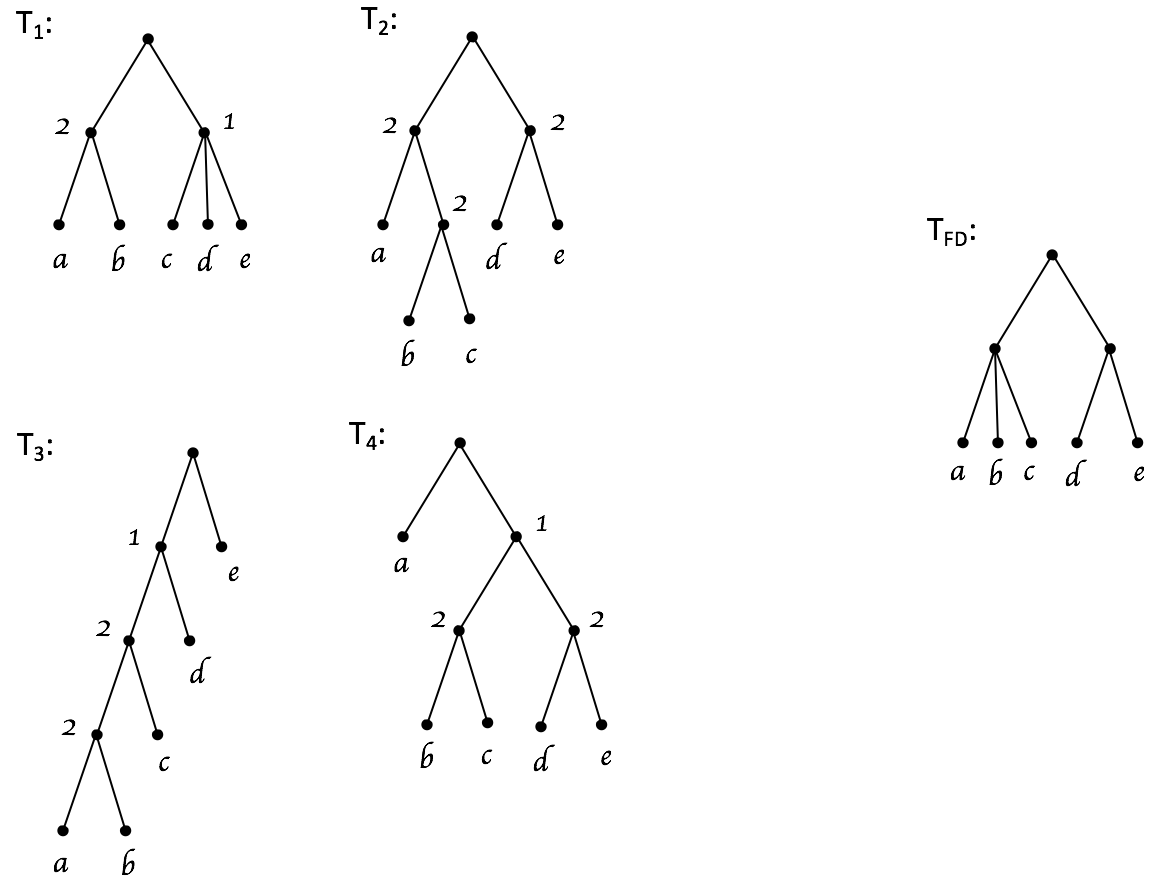
\includegraphics[scale=0.5]{freqdiff}
        \centering
        \caption[Example of a frequency difference consensus tree]{Let $\mathcal{S} = \{T_1, T_2, T_3, T_4\}$. $T_{FD}$ is the FDCT of $\mathcal{S}$. The number beside each non-root internal node $u$ indicates the weight of the node, $\weight(u)$, which is the number of occurences of the cluster $\leafset(u)$ in $\mathcal{S}$.}
        \label{fig:freqdiff}
    \end{figure}

    A \textit{frequency difference consensus tree} is defined as follows. Let $\mathcal{S}$ be a set of $k$ trees with identical leaf labels, i.e. $\mathcal{S} = \{T_1, T_2, \ldots, T_k\}$, where $\leafset(T_1) = \leafset(T_2) = \ldots = \leafset(T_k) = L$. For any cluster $C \subseteq L$, let weight of $C$, denoted as $\weight(C)$, be $|\{T : T \in \mathcal{S} \text{ and } C \in \mathcal{C}(T)\}|$, i.e. the number of trees in $\mathcal{S}$ which $C$ occurs in. For convenience, we also define, for any tree $T \in \mathcal{S}$, for any node $u \in V(T)$, the weight of $u$, denoted as $\weight(u)$ to be $\weight(\leafset^{T}(u))$. Then the FDCT of $\mathcal{S}$ is the tree $T_{FD}$, where $\mathcal{C}(T_{FD}) = \{C : C \subseteq L \text{ and } \weight(C) > max(\{\weight(C_1) : C_1 \subseteq L \text{ and } C \not\compatible C_1\})\}$. Thus $T_{FD}$ contains all clusters that occur more frequently than any cluster that they are incompatible with. By Proposition $3$ in \cite{steel2014axiomatic}, this tree always exists and is unique for a given $\mathcal{S}$. Figure~\ref{fig:freqdiff} gives an example. In this, $\weight(\{a, b\}) = 2 \leq \weight(\{b, c\}) = 2$ and $\{a, b\} \not\compatible \{b, c\}$, hence $\{a, b\}$ is not in the final consensus tree. However $\{a, b, c\}$ and $\{d, e\}$ have frequencies greater than any cluster incompatible with them, hence they both exist in the consensus tree. Note that frequencies are not shown for the trivial clusters.

    For each of the definitions above where the tree is specified in the superscript, this superscript is omitted if the tree being referred to is clear from context. For example, $children^T(u)$ would be written as $children(u)$. This will also be applied to any notation developed in the remainder of this text.

    Henceforth, $\mathcal{S}$ is taken to be the input set of trees with identical leaf labels. This set of leaf labels is denoted by $L$. Let $|\mathcal{S}| = k$ and $|L| = n$.

    \subsection{Previous Work}
    \label{subsec:previouswork}

    An implementation of the FDCT can be found in the free software package TNT \cite{goloboff2008tnt}; however the algorithm used within is unavailable and so its complexity is not known. Jansson et al. \cite{jansson2018algorithms} gave a deterministic $min\{O(kn^2), O(kn(k + log^2 n))\}$ algorithm for constructing the FDCT, implemented in the open source FACT package \cite{jansson2016improved}. Gawrychowski et al. \cite{gawrychowski2017faster} improved upon this to give a deterministic $O(kn\,log^2n)$ algorithm (not yet implemented).

    \subsection{Organisation of the Article and New Results}

    {\bf KEN: It is important to state that the time improvement is challenging. Can you high-light the techniques that lead to the improvement here?}

    Section~\ref{sec:preliminaries} contains some results from previous works that are utilised later.
    Section~\ref{sec_freq_diff_algo} gives the framework of the FDCT construction algorithm that runs in $O(kn\,log\,n)$ time.
    Sections~\ref{sec:weighting} and~\ref{sec:filterclusters} present algorithms for solving subproblems of the FDCT construction.
    Section~\ref{sec:rmqtree} shows how an efficient data structure can be built on trees; this will be utilised later.
    Finally, Section~\ref{sec:implementation} details how the algorithm was implemented and presents some experimental results.

    \section{Preliminaries}
    \label{sec:preliminaries}

    \subsection{The \textit{lca} operation}

    We restate the following lemma outlining the \textit{lca} operation from \cite{bender2000lca}:
%    \newline

    \begin{lemma}
        \label{lem:lca}
        Given any tree $T$, the $lca$ data structure can be constructed in $O(n)$ time, where $n = |V(T)|$. Then, for any nodes $u, v \in V(T)$, the query $lca^{T}(u, v)$ can be answered in constant time.
    \end{lemma}


%    \subsection{The linear RMQ (range minimum/maximum) data structure}

%    For any array $A[1 \ldots n]$ of length $n$ and any indices $i, j$, $1 \leq i \leq j \leq n$, let $rmq^A(i, j)$ denote $max_{i \leq k \leq j}A[k]$. We restate the following lemma about answering $rmq$ queries from \cite{bender2000lca}:
%    \newline


    \subsection{Centroid Path Decomposition}

    The \textit{centroid path decomposition technique} of \cite{cole2000n} is used to decompose a tree $T$ into a path from the root to some leaf and a set of disjoint subtrees. For any $u \in V(T)$, we define the \textit{heaviest child} of $u$, denoted by $heavyChild(u)$, to be the one with the largest leafset, with ties broken arbitrarily. The remaining children are called the \textit{side children} of $u$, denoted by $sideChildren(u)$. A \textit{centroid path} in $T$ is the path formed by starting at the root and at each point following the heaviest child. The centroid path is denoted by $\pi(T) = \langle p_{\gamma}, p_{\gamma - 1}, \ldots, p_1 \rangle$, where $p_{\gamma}$ is the root of $T$ and $p_1$ is a leaf. Removing the path $\pi(T)$ from $T$ results in a set of disjoint subtrees of $T$, where the root of each such subtree is a child of some node in $\pi(T)$. These trees are called the \textit{side trees} of $\pi(T)$, denoted by $\sigma(T)$. Also, for any node $u \in V(T)$, let $\sigma(u)$ be the set of trees rooted at $sideChildren(u)$, called the side trees \textit{associated} with $u$. Figure~\ref{fig:centroid}(a) demonstrates this decomposition. Here, the bold path from the root to leaf is the centroid path. When the dashed edges and the nodes contained in the centroid path are removed from the tree, the side trees remain. In particular, it can be seen that there are two side trees associated with the root, one containing just a single leaf, while the other is a larger tree. {\bf KEN: I don't understand "In particular, ... larger tree." May be can remove it.}

    {\bf KEN: Can we avoid complete centroid path decomposition? If yes, we can remove Figure 2(b) and the following paragraph.}

    We further define a \textit{complete centroid path decomposition} for any tree $T$. Here, the normal centroid path decomposition is applied on $T$, and then each side tree is recursively decomposed. This results in a set of disjoint paths in $T$, denoted by $\mathcal{P}(T)$. We also assign each path $P_i \in \mathcal{P}(T)$ a depth, denoted as $depth^{T}(P_i)$, defined to be $1\, +$ depth of centroid path containing the parent of the root of $P_i$. Intuitively, if we build a tree from only the roots of the centroid paths while maintaining the same relative structure, then the depth of a centroid path would simply be the depth of its root in this new tree. Figure~\ref{fig:centroid}(b) applies complete centroid path decomposition on the same tree as before. The bold paths, along with the isolated leaves, are centroid paths. As can be seen, the large side tree that remained intact in Figure~\ref{fig:centroid}(a) has now been recursively decomposed. The depth of each centroid path is shown next to its root.

    \begin{figure}[ht]
        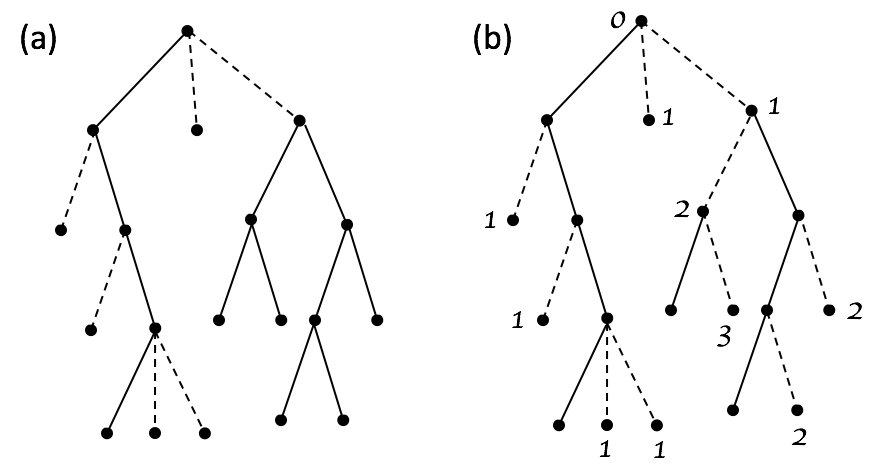
\includegraphics[scale=0.5]{centroid}
        \centering
        \caption[Centroid path decomposition]{Demonstration of centroid path decomposition. Both (a) and (b) use the same tree. In (a), the tree has undergone a centroid path decomposition such that after the dashed edges are removed, leaving a centroid path and a set of side trees. In (b), the tree has undergone a complete centroid path decomposition, with the dashed edges being removed to leave only a set of paths. The depth of each centroid path is shown next to its root.}
        \label{fig:centroid}
    \end{figure}

    \subsection{The \textit{delete} operation}
    \label{subsec:delete}

    {\bf KEN: Do we still need the delete operation? If not, we can remove this section.}

    As described in \cite{jansson2018algorithms}, the \textit{delete} operation deletes a cluster from a tree. To do so, we specify some internal node $u$ in a tree $T$, such that we wish to delete the cluster $\leafset^{T}(u)$. Then the \textit{delete} operation makes $parent(u)$ the parent of all nodes in $children(u)$ and removes $u$, along with any associated edges from $T$. This has the effect of removing only $\leafset(u)$ from $T$, without affecting any other cluster. For example, in Figure~\ref{fig:freqdiff}, if we perform a delete operation on $T_2$, on the node associated with the cluster $\{b, c\}$, the resulting tree is identical to $T_{FD}$.

    \subsection{Restricted Trees}
    \label{subsec:restrictedtree}

    For any tree $T$ and any cluster $C \subseteq \leafset(T)$, define $T|C$, read as ``$T$ restricted to $C$'', as the tree $T'$ with $V(T') = \{lca^T(u, v) : u, v \in C\}$ which obeys $lca^T(C') = lca^{T'}(C')$ for all $C' \subseteq C$. Intuitively, $T'$ has the leaf set $C$ and consists of all nodes in $T$ that are $lca$'s of the leaves in $C$, with these nodes connected such that they have the same ancestor/descendant relationships as they had in $T$. Figure~\ref{fig:restrictedtree} demonstrates this process. Notice that nodes which are not $lca$'s of the cluster are removed, but the structure of the tree in relation to the leaves in the cluster remains the same.

    \begin{figure}[ht]
        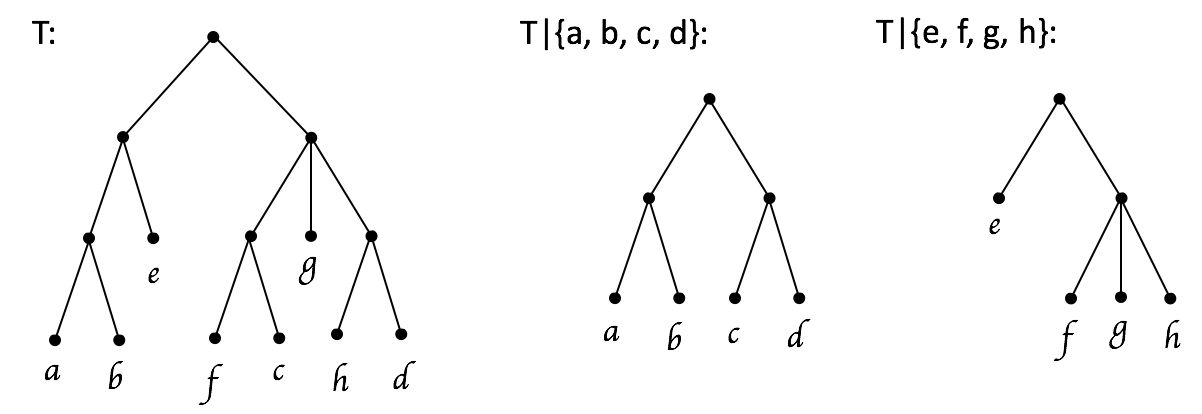
\includegraphics[scale=0.5]{restrictedsubtree}
        \centering
        \caption[Restricted Trees]{Illustration of restricting a tree to a cluster. The tree $T$, along with $T|\{a, b, c, d\}$ and $T|\{e, f, g, h\}$ are shown.}
        \label{fig:restrictedtree}
    \end{figure}

%    \subsection{Characterising incompatibility}
%
%    For any tree $T$ and cluster $C \subseteq \leafset(T)$, define the set $Conflict^{T}(C) = \{u : u \in V(T) \text{ and } \leafset^{T}(u) \not\compatible C\}$. Lemma 6 of \cite{jansson2018algorithms}, which gives a property of this set, is restated here since it is crucial in the development of an algorithm discussed below.
%    \newline
%
%    \begin{lemma}
%        \label{lem:incompatibility}
%        Given a tree $T$ and a cluster $C \subseteq \leafset(T)$, let $l_C = lca^T(C)$. Then for any $u \in V(T)$, $u \in Conflict^{T}(C)$ iff $u$ lies on the path between $l_C$ and some $x \in C$ and $\leafset(u) \not\subseteq C$.
%    \end{lemma}

%    \subsection{The \texttt{Merge\_Trees} algorithm}
%    \label{subsec:mergetrees}

%    We restate the following lemma outlining the \texttt{Merge\_Trees} operation from \cite{jansson2016improved}:
%    \newline
%
%    \begin{lemma}
%        \label{lem:mergetrees}
%        Given two trees $T_1$ and $T_2$ where $\leafset^{T_1} = \leafset^{T_2} = L$ and $T_1 \compatible T_2$, \texttt{Merge\_Trees}$(T_1, T_2)$ returns a tree $T$ such that $\leafset^T = L$ and $\mathcal{C}(T) = \mathcal{C}(T_1) \cup \mathcal{C}(T_2)$. This algorithm runs in $O(|L|)$ time.
%    \end{lemma}
%
%    \begin{figure}[ht]
%        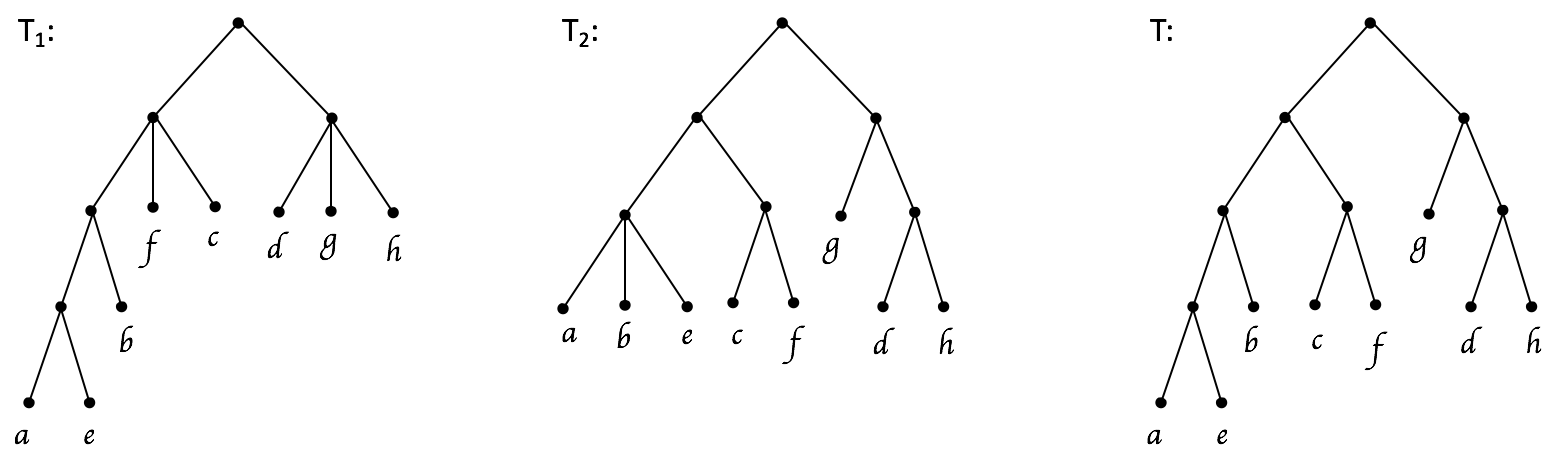
\includegraphics[scale=0.5]{mergetrees}
%        \centering
%        \caption[The \texttt{Merge\_Trees} algorithm]{$T_1 \compatible T_2$. $T =$ \texttt{Merge\_Trees}$(T_1, T_2)$. $\mathcal{C}(T) = \mathcal{C}(T_1) \cup \mathcal{C}(T_2)$.}
%        \label{fig:mergetrees}
%    \end{figure}
%
%    Figure~\ref{fig:mergetrees} gives an example for the \texttt{Merge\_Trees} algorithm. Here, $T_1 \compatible T_2$ and $T =$ \texttt{Merge\_Trees}$(T_1, T_2)$. Observe that,
%    \begin{align*}
%        \mathcal{C}(T_1) &= \{\{a, e\}, \{a, b, e\}, \{a, b, c, e, f\}, \{d, g, h\}\}\\
%        \mathcal{C}(T_2) &= \{\{a, b, e\}, \{c, f\}, \{a, b, c, e, f\}, \{d, h\}, \{d, g, h\}\}\\
%        \mathcal{C}(T) &= \{\{a, e\}, \{a, b, e\}, \{c, f\}, \{a, b, c, e, f\}, \{d, h\}, \{d, g, h\}\}\\
%        &= \mathcal{C}(T_1) \cup \mathcal{C}(T_2).
%    \end{align*}

    \section{The \texttt{Frequency\_Difference} algorithm}
    \label{sec_freq_diff_algo}

    Given a set of trees $\mathcal{S} = \{ T_1, \ldots, T_k \}$ where $\Lambda(T_1) = \ldots = \Lambda(T_k) = L$, this section describes the overall framework to compute the FDCT of $\mathcal{S}$, which is proposed by \cite{jansson2018algorithms}.
    The algorithm \texttt{Frequency\_Difference} runs in three phases.

    The first phase is the \textit{weighting} step. It computes, for any tree $T_i \in \mathcal{S}$ and any node $u \in V(T_i)$, $\weight(u) = | \{ T_j \in {\cal S} \mid \Lambda(T_i[u]) \in \mathcal{C}(T_j) \} |$. Jansson et al. \cite{jansson2018algorithms} gave a $min(\{O(kn^2), O(k^2n)\})$ solution to the weighting step.
    Gawrychowski et al. \cite{gawrychowski2017faster} improved the runtime of the weighting step to $O(kn\,log^2n)$. In Section~\ref{sec:weighting}, we give the proof of the following lemma which shows that the weighting step can be solved in $O(k n \log n)$ time.

    \begin{lemma}
	    \label{lem-weighting-time}
	   The weighting step takes $O(kn \log n)$ time.
    \end{lemma}

    Now, we assume every cluster (or every node) in the trees in $\mathcal{S}$ is associated with a weight. The second phase computes the forward frequency difference consensus tree (FFDCT) of a list of trees $(T_1, T_2, \ldots, T_k)$.
    The FFDCT of $(T_1, T_2, \ldots, T_k)$ is defined as the tree that includes, for every $1 \leq i \leq k$, every cluster $C \in \mathcal{C}(T_i)$ that satisfies $\weight(C) > \weight(X)$ for all $X \in \bigcup_{j=i}^k \mathcal{C}(T_j)$ with $C \not\compatible X$. Below lemma states a recursive formula to compute $FFDCT(T_1, \ldots, T_k)$. Note that the output of $FFDCT()$ depends on the ordering of the trees.

    \begin{lemma} \label{lem-FFDCT}
	    Let $T = FFDCT(T_1, \ldots, T_{k-1})$. Then, $FFDCT(T_1, \ldots, T_k) = FFDCT(T, T_k)$.
    \end{lemma}


    $FFDCT(T_1, T_2)$ can be computed by utilising \texttt{Filter\_Clusters} and \texttt{Merge\_Trees} (defined below).

    Given two trees $T_1$ and $T_2$ where $\leafset^{T_1} = \leafset^{T_2} = L$ and $T_1 \compatible T_2$, \texttt{Merge\_Trees}$(T_1, T_2)$ returns a tree $T$ such that $\leafset^T = L$ and $\mathcal{C}(T) = \mathcal{C}(T_1) \cup \mathcal{C}(T_2)$. Figure~\ref{fig:mergetrees} gives an example for the \texttt{Merge\_Trees} algorithm.

    \begin{figure}[ht]
        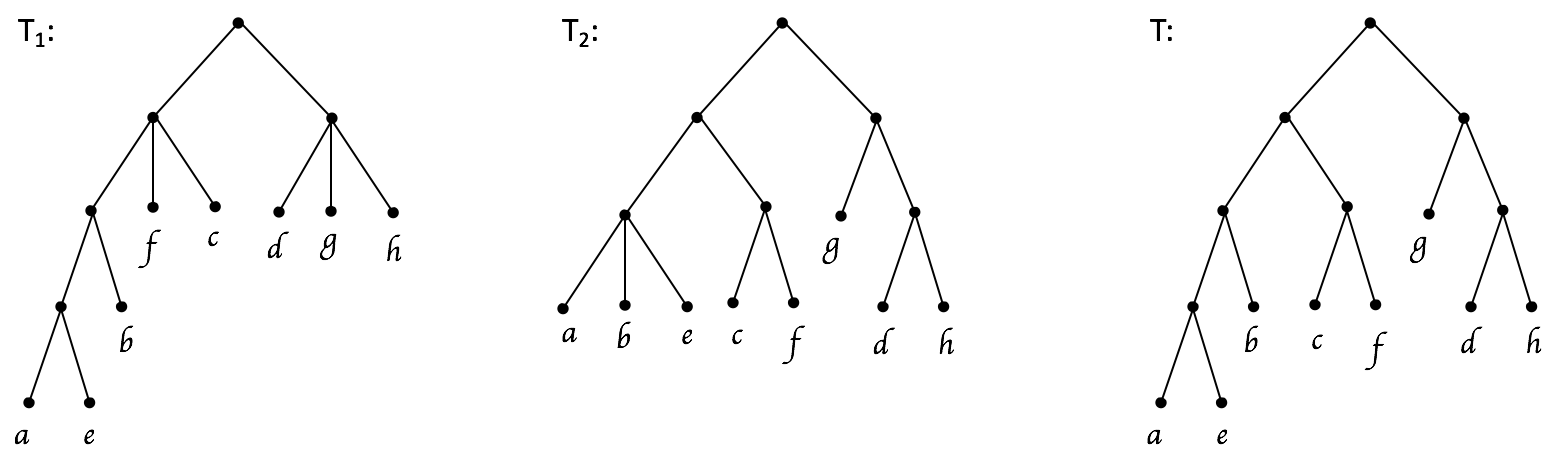
\includegraphics[scale=0.5]{mergetrees}
        \centering
        \caption[The \texttt{Merge\_Trees} algorithm]{$T_1 \compatible T_2$. $T =$ \texttt{Merge\_Trees}$(T_1, T_2)$. $\mathcal{C}(T) = \mathcal{C}(T_1) \cup \mathcal{C}(T_2)$.}
        \label{fig:mergetrees}
    \end{figure}
    Jansson et al.\cite{jansson2016improved} showed that the operator \texttt{Merge\_Trees} runs in $O(|L|)$ time.

    The subprocedure \texttt{Filter\_Clusters} is defined to take as input trees $\TA$ and $\TB$, with $\leafset^{\TA} = \leafset^{\TB} = L$ and the values of $\weight(u)$ for all $u \in V(\TA) \cup V(\TB)$. It returns a tree $T$ which contains all clusters $C$ in $\TA$ for which $\weight(C) > $ weights of all clusters in $\TB$ that are incompatible with $C$. Formally, \texttt{Filter\_Clusters}$(\TA, \TB) = T$ where $\mathcal{C}(T) = \{C : C \in \mathcal{C}(\TA) \text{ and } \weight(C) > max(\{\weight(C_1) : C_1 \in \mathcal{C}(\TB) \text{ and } C_1 \not\compatible C\})\}$ and $\leafset^T = L$. For example, referring to Figure~\ref{fig:freqdiff}, \texttt{Filter\_Clusters}$(T_2, T_1) = T_{FD}$. Notice that there are three non-trivial clusters in $T_2$: $\{a, b, c\}, \{b, c\}$ and $\{d, e\}$. All of these have weight $2$. Now the only cluster in $T_1$ incompatible with $\{a, b, c\}$ is $\{c, d, e\}$, but this only has weight $1$ and so $\{a, b, c\}$ is kept. The cluster $\{d, e\}$ is compatible with $T_1$ so it is also kept. However, $\{b, c\}$ is incompatible with $\{a, b\}$ and they both have weight $2$, hence $\{b, c\} \not\in \mathcal{C}($\texttt{Filter\_Clusters}$(T_2, T_1))$.

    \cite{jansson2018algorithms} gave an $O(n\,log^2n)$ solution to \texttt{Filter\_Clusters}. In Section~\ref{sec:filterclusters}, we give the following lemma.
    In Section~\ref{sec:filterclusters}, we give the proof of the following lemma which shows that $Filter\_Cluster$ of two trees can be computed in $O(n \log n)$ time.
    \begin{lemma}
	    \label{lem-filter-cluster-time}
	    Given two weighted trees $T_1$ and $T_2$ of size $n$,
	    $Filter\_Cluster(T_1, T_2)$ can be computed in $O(n \log n)$ time.
    \end{lemma}

    Below lemma states the relationship between $FFDCT$, $Filter\_Clusters$ and $Merge\_Trees$.
    \begin{lemma}
	    \label{lem-FFDCT-merge-filter}
	    $FFDCT(T_1, T_2) = Merge\_Trees( Filter\_Clusters(T_1, T_2), Filter\_Clusters(T_2, T_1) )$.
    \end{lemma}


    Given the FFDCT of $(T_1, \ldots, T_k)$, the third phase computes the FDCT of $\{ T_1, \ldots, T_k \}$. Below lemma states how can we compute FDCT utilizing $Filter\_Clusters$.
    \begin{lemma}
	    \label{lem-FDCT}
	    Let $T$ be the FFDCT of $(T_1, \ldots, T_k)$.

    \end{lemma}



    In conclusion, we have the following theorem.
    \begin{theorem}
    The FDCT of $\{T_1, \ldots, T_k\}$ can be computed in $O(kn \log n)$ time.
    \end{theorem}
    \begin{proof}
	    There are three phases.
	    Phase 1 takes $O(k n \log n)$ time by Lemma~\ref{lem-weighting-time}.

	    By Lemmas~\ref{lem-FFDCT}, \ref{lem-filter-cluster-time} and \ref{lem-FFDCT-merge-filter}, we conclude that Phase 2 computes the FFDCT of $(T_1, \ldots, T_k)$ using $O(k n \log n)$ time.


	    Given the FFDCT of $(T_1, \ldots, T_k)$, by Lemmas~\ref{lem-FDCT} and \ref{lem-filter-cluster-time}, we can build the FDCT of $\{T_1, \ldots, T_k\}$ in $O(kn \log n)$ time.
	    The lemma follows.
    \end{proof}

    To complete the proof of the above theorem, Sections~\ref{sec:weighting} and \ref{sec:filterclusters} shows the correctness of Lemmas~\ref{lem-weighting-time} and \ref{lem-filter-cluster-time}.

%    \cite{jansson2018algorithms} shows that Algorithm~\ref{alg:frequencydifference} correctly reconstructs the FDCT of ${\cal S} = \{T_1, \ldots, T_k\}$.
    %The \texttt{Frequency\_Difference} algorithm is given in Algorithm~\ref{alg:frequencydifference}.

%    \begin{algorithm}
%        \caption{Frequency\_Difference}
%        \label{alg:frequencydifference}
%
%        \begin{algorithmic}[1]
%            \Input A set $\mathcal{S}$ of trees $\{T_1, T_2, \ldots, T_k\}$ where $\leafset(T_1) = \leafset(T_2) = \ldots = \leafset(T_k) = L$
%
%            \Output A tree $T_{FD}$, where $\mathcal{C}(T_{FD}) = \{C : C \subseteq L \text{ and } \weight(C) > max(\{\weight(C_1) : C_1 \subseteq L \text{ and } C \not\compatible C_1\})\}$ and $\leafset^{T_{FD}} = L$.
%
%            \State Compute $\weight(C)$ for every cluster $C$ that occurs in $S$.
%
%            \State $T := T_1$
%
%            \For{$j := 2$ to $k$}
%                \State $A :=$ \texttt{Filter\_Clusters}$(T, T_j)$
%
%                \State $B :=$ \texttt{Filter\_Clusters}$(T_j, T)$
%
%                \State $T :=$ \texttt{Merge\_Trees}$(A, B)$
%            \EndFor
%
%            \For{$j := 1$ to $k$}
%                \State $T :=$ \texttt{Filter\_Clusters}$(T, T_j)$
%            \EndFor
%
%            \State \Return $T$
%        \end{algorithmic}
%    \end{algorithm}

%    Theorem 3 of \cite{jansson2018algorithms} gives the following corollary which give the running time:
%    \newline

%    \begin{corollary}
%        \label{cor:freqdiffruntimecomponents}
%        The total runtime of \texttt{Frequency\_Difference} is given by $O(g(n, k) + k \cdot f(n))$ where $g(n, k)$ is the time taken by the weighting step and $f(n)$ is the runtime of \texttt{Filter\_Clusters}.
%    \end{corollary}

%    Jansson et al. \cite{jansson2018algorithms} gave a $min(\{O(kn^2), O(k^2n)\})$ solution to the weighting step and an $O(n\,log^2n)$ solution to \texttt{Filter\_Clusters}, giving an overall runtime of $min(\{O(kn^2), O(kn(k + log^2n))\})$. Gawrychowski et al. \cite{gawrychowski2017faster} improved the runtime of the weighting step to $O(kn\,log^2n)$, thus reducing the overall runtime to $O(kn\,log^2n)$.


    \section{Weighting}
    \label{sec:weighting}

    Given the set of trees $\mathcal{S} = \{T_1, T_2, \ldots, T_k\}$, where $\leafset(T_1) = \leafset(T_2) = \ldots = \leafset(T_k) = L$ and $n = |L|$, the weighting step computes $\weight(u)$ for every node $u \in V(T)$, $T \in \mathcal{S}$. Recall that $\weight(u)$ gives the frequency of $\leafset^T(u)$ in $\mathcal{S}$. We divide this work (as in \cite{gawrychowski2017faster}) into the labelling and counting steps. The labelling step assigns an integer label to each node $u \in T, T \in \mathcal{S}$, denoted by $id(u)$, such that $1 \leq id(u) \leq 2kn$ and for any node $u' \in T', T' \in \mathcal{S}$, $id(u) = id(u')$ iff $\leafset^T(u) = \leafset^{T'}(u')$. That is, two nodes have the same label iff they are associated with the same cluster. The counting step sorts these labels, allowing us to count how many nodes exist with each label, giving us the frequencies (or the weights) of the nodes.

    Recall that the approach in \cite{gawrychowski2017faster} costs $O(kn\,log^2n)$ time. Below, we develop a way to achieve $O(kn\,log\,n)$ time.

    We first define a mapping $assoc$. Let $L'$ and $L''$ be a partition of $L$ such that $L = L' \cup L''$ and $|L'|=|L''|$.
    For any tree $T_i \in \mathcal{S}$, for any node $u \in V(T_i)$, $assoc^{L'}(u)$ aims to map $u$ to the corresponding node in $T_i|L'$. Formally, if $\Lambda^{T_i}(u) \cap L' \neq \emptyset$,
    define $assoc^{L'}(u)$ be the node $v \in V(T|L')$ such that $\Lambda^T(u) \cap L' = \Lambda^{T|L'}(v)$; otherwise, define $assoc^{L'}(u)$ be $\Phi$, where $\Phi$ is a special node with $id(\Phi) = 0$.
    $assoc^{L''}$ can be defined analogically.  We refer to Figure~\ref{fig:labelclusters} to show examples of this concept. Let $u$ and $v$ be the nodes in $T_1$ labelled $(5, 1)$ and $(5, 0)$ respectively. Then $assoc^{\{a, b, c, d\}}(u) = v$, since $v = lca^{T_1}(\{a, b, c, d\} \cap \leafset^{T_1}(u)) = lca^{T_1}(\{a, b\})$. $assoc^{\{e, f, g, h\}}(v) = \Phi$, since $\leafset^{T_1}(v) \cap \{e, f, g, h\} = \emptyset$.

    {\bf KEN: I think the above example for $assoc$ is not correct!}

    \begin{lemma}
        \label{lem:labelclusterscorrectness}
        Given any trees $T_i, T_j \in \mathcal{S}$, for any nodes $u \in V(T_i), v \in V(T_j)$, $(id(assoc^{L'}(u)), id(assoc^{L''}(u))) = (id(assoc^{L'}(v)), id(assoc^{L''}(v)))$ iff $\leafset^{T_i}(u) = \leafset^{T_j}(v)$.
    \end{lemma}
        \begin{proof}
		($\leftarrow$) If $\leafset^{T_i}(u) = \leafset^{T_j}(v)$, we have $\leafset^{T_i|L'}(assoc^{L'}(u)) = \leafset^{T_j|L'}(assoc^{L'}(v))$ and $\leafset^{T_i|L''}(assoc^{L''}(u)) = \leafset^{T_j|L''}(assoc^{L''}(v))$. Hence, we have $(id(assoc^{L'}(u)), id(assoc^{L''}(u))) = (id(assoc^{L'}(v)), id(assoc^{L''}(v)))$.

		($\rightarrow$) If $(id(assoc^{L'}(u)), id(assoc^{L''}(u))) = (id(assoc^{L'}(v)), id(assoc^{L''}(v)))$, we have $\Lambda^{T_i}(u) \cap L' = \Lambda^{T_j}(v) \cap L'$ and $\Lambda^{T_i}(u) \cap L'' = \Lambda^{T_j}(v) \cap L''$. This implies  $\leafset^{T_i}(u) = \leafset^{T_j}(v)$.
%            Inductively, $id(assoc^{L'}(u)) = id(assoc^{L'}(v))$ iff $\leafset^{T_i|L'}(assoc^{L'}(u)) = \leafset^{T_j|L'}(assoc^{L'}(v))$. By definition of the $assoc$ relation, $\leafset^{T_i}(u)\, \cap\, L' = \leafset^{T_j}(v)\, \cap\, L'$. Symmetrically, $id(assoc^{L''}(u)) = id(assoc^{L''}(v))$ iff $\leafset^{T_i}(u)\, \cap\, L'' = \leafset^{T_j}(v)\, \cap\, L''$. Since $L'$ and $L''$ partition $L$, both parts are true iff $\leafset^{T_i}(u) = \leafset^{T_j}(v)$.
        \end{proof}


    Using the above observation, the labeling problem can be solved using a divide and conquer strategy. Let \texttt{Label\_Trees}$(\{T_1, T_2, \dots, T_k\})$ be the procedure to compute the labels for all nodes in the trees.
    %We partition $L$ into two equal sized halves, $L'$ and $L''$ such that $L = L' \cup L''$.
    We recursively call \texttt{Label\_Trees}$(\{T_1|L', T_2|L', \dots, T_k|L'\})$ and \texttt{Label\_Trees}$(\{T_1|L'', T_2|L'', \dots, T_k|L''\})$ and obtain labels for all nodes in $T_i|L'$ and $T_i|L''$ for $i=1, \ldots, k$.
    %The first call gives us labels for the set of clusters $\{\leafset^{T|L'}(u) : T \in \mathcal{S}, u \in V(T|L')\}$, which turns out to be equivalent to the set $\{\leafset^{T}(u) \cap L' : T \in \mathcal{S}, u \in V(T)\}$. Similarly, the second call gives labels for the set of clusters $\{\leafset^{T}(u) \cap L'' : T \in \mathcal{S}, u \in V(T)\}$.
    Then for any tree $T_i \in \mathcal{S}$, for any node $u \in V(T_i)$, Lemma~\ref{lem:labelclusterscorrectness} implies that $\leafset^{T_i}(u)$ is uniquely identified by the pair $(id(assoc^{L'}(u)), id(assoc^{L''}(u))$.
    We sort all pairs and assign a rank to each unique pair; $id(u)$ is then the rank of the pair $(id(assoc^{L'}(u)), id(assoc^{L''}(u)))$. Algorithm~\ref{alg:labelclusters} details the pseudocode for \texttt{Label\_Trees}.

%    For every cluster $C \subseteq L$, and every node $u$ in $T$, define $assoc^C(u)$ be the node $lca^T(C \cap \leafset^T(u))$ if $C \cap \leafset^T(u) \neq \emptyset$; otherwise, define $assoc^C(u)$ be $\Phi$, where $\Phi$ is a special node with $id(\Phi) = 0$ and $\leafset(\Phi) = \emptyset$. We refer to Figure~\ref{fig:labelclusters} to show examples of this concept. Let $u$ and $v$ be the nodes in $T_1$ labelled $(5, 1)$ and $(5, 0)$ respectively. Then $assoc^{\{a, b, c, d\}}(u) = v$, since $v = lca^{T_1}(\{a, b, c, d\} \cap \leafset^{T_1}(u)) = lca^{T_1}(\{a, b\})$. $assoc^{\{e, f, g, h\}}(v) = \Phi$, since $\leafset^{T_1}(v) \cap \{e, f, g, h\} = \emptyset$.
%    \newline


%    Using this observation, we can expand on the previous description of the algorithm. As mentioned above, we first obtain, for every $T \in \mathcal{S}$, for every node $u \in V(T)$, the pair $(id(assoc^{L'}(u)), id(assoc^{L''}(u)))$. Then we sort them and assign a rank to each unique pair; $id(u)$ is then the rank of the pair $(id(assoc^{L'}(u)), id(assoc^{L''}(u)))$. The resulting algorithm \texttt{Label\_Trees} is laid out below.

    \begin{algorithm}
        \caption{Label\_Trees}
        \label{alg:labelclusters}

        \begin{algorithmic}[1]
            \Input A set $\mathcal{S}$ of trees $\{T_1, T_2, \dots, T_k\}$ where $\leafset(T_1) = \leafset(T_2) = \dots = \leafset(T_k) = L$

	    \Output Associate a label $id(u) \in \{1, \dots, 2k |L| \}$ with every node $u$ in the trees in $\mathcal{S}$ such that for any two nodes $v, w$ in some trees in $\mathcal{S}$, $id(v) = id(w)$ iff $\leafset(v) = \leafset(w)$.

            \State Partition $L$ into $L'$ and $L''$ such that $|L'| = |L''|$.

            \State For all $i \in [1 \dots k]$, let $T'_i = T_i|L'$ and $T''_i = T_i|L''$.

            \State \texttt{Label\_Trees}$(\{T'_1, T'_2, \dots, T'_k\})$.

            \State \texttt{Label\_Trees}$(\{T''_1, T''_2, \dots, T''_k\})$.

            \State For every tree $T \in \mathcal{S}$, for every node $u \in T$, represent $u$ by the pair $(id(assoc^{L'}(u)), id(assoc^{L''}(u)))$.

            \State Radix sort all pairs obtained and remove duplicates. Assign a rank to each unique pair.

            \State For every tree $T \in \mathcal{S}$, for every node $u \in T$, set $id(u) = $ rank of the pair $(id(assoc^{L'}(u)), id(assoc^{L''}(u)))$.
        \end{algorithmic}
    \end{algorithm}

    Figure~\ref{fig:labelclusters} illustrates one iteration of \texttt{Label\_Trees}. Here $L' = \{a, b, c, d\}$ and $L'' = \{e, f, g, h\}$. It is assumed that the algorithm has correctly labelled the nodes for each of the restricted trees, and these labels are assigned as shown in Figure~\ref{fig:labelclusters}(b). Figure~\ref{fig:labelclusters}(a) then shows the pair associated with each internal node of $T_1$ and $T_2$. For example, the cluster $\{a, b, e\}$ in $T_1$ is labelled by $5$ from $\{a, b\}$ in $T_1|L'$ and $1$ from $\{e\}$ in $T_1|L''$. Similarly, the cluster $\{a, b\}$ in $T_1$ is labelled by $5$ from $\{a, b\}$ in $T_1|L'$ and $0$ from $\Phi$ since $\{a, b\} \cap \{e, f, g, h\} = \emptyset$.

    \begin{figure}[ht]
        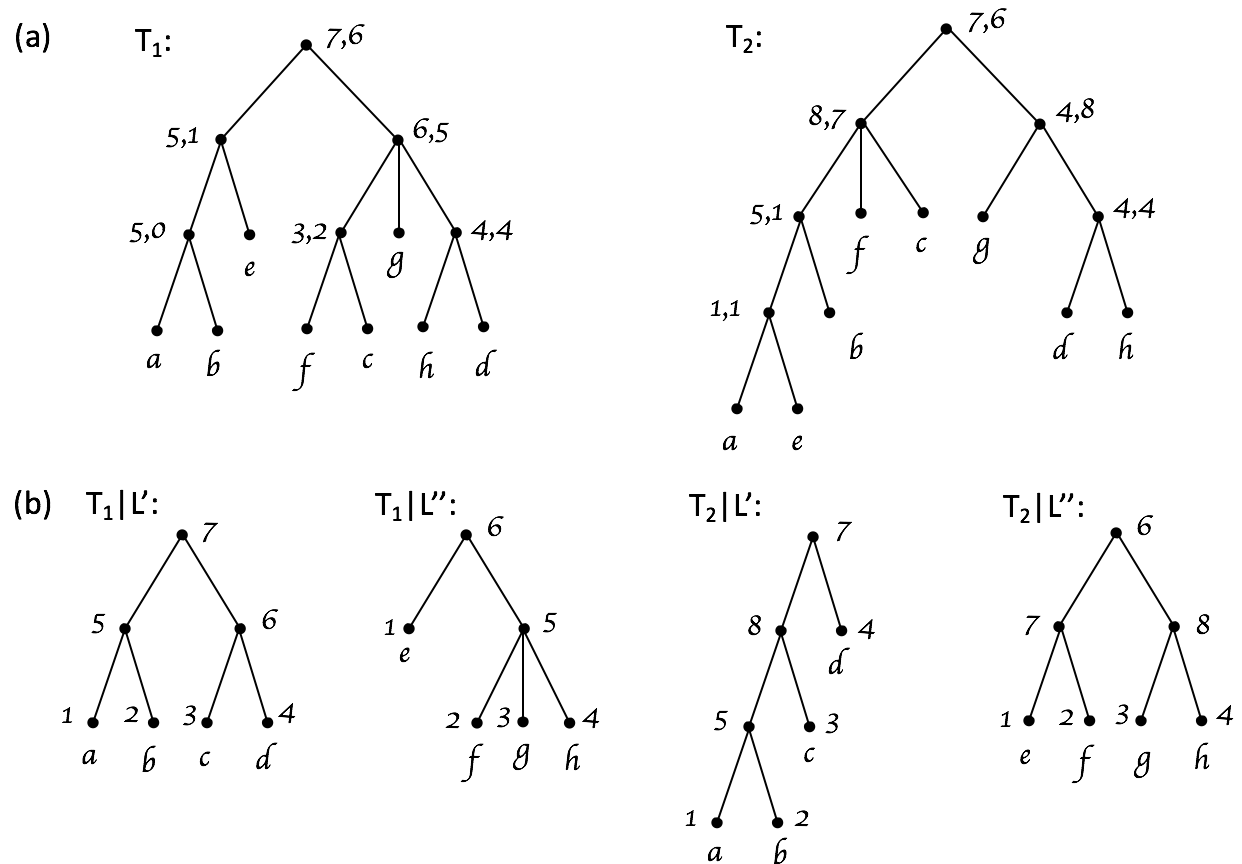
\includegraphics[scale=0.5]{labelclusters}
        \centering
        \caption[The \texttt{Label\_Trees} algorithm]{Demonstration of \texttt{Label\_Trees}$(T_1, T_2)$. $L' = \{a, b, c, d\}$ and $L'' = \{e, f, g, h\}$. (b) shows the trees $T_1|L', T_1|L'', T_2|L'$ and $T_2|L''$, where these have been recursively labelled. The labels are shown beside each of the nodes. (a) shows the trees $T_1$ and $T_2$ where the pair that represents each node (except the leaves) is shown beside it.}
        \label{fig:labelclusters}
    \end{figure}

    \bigskip
    \begin{lemma}
        \label{lem:labelclustersidbounds}
	    After running \texttt{Label\_Trees}$(\mathcal{S})$, for any node $u \in V(T), T \in \mathcal{S}$, $id(u) \in \{1, \dots, 2k |L|\}$.
    \end{lemma}
        \begin{proof}
            It is easily seen that $|V(T)| < 2|L|$. Thus the total number of pairs is less than $2k|L|$. This also places an upper bound on the number of ids. Notice that $u$ cannot be labelled with $0$ since that is reserved for the special node.
        \end{proof}

    \medskip
    \begin{lemma}
        \label{lem:labelclustersruntime}
        The algorithm \texttt{Label\_Trees}$(\mathcal{S})$ runs in $O(kn\,log\,n)$ time.
    \end{lemma}
        \begin{proof}
            Let $T(m)$ be the runtime of \texttt{Label\_Trees}$(\mathcal{S})$, where $m =$ size of leaf set of each tree in $\mathcal{S}$. By Lemma 5.2 of \cite{farach1995fast}, construction of $T'_i$ and $T''_i$ takes $O(m)$ time for each $T_i \in \mathcal{S}$, taking total $O(km)$ time over all the trees. Computing $assoc^{L'}(u)$ and $assoc^{L''}(u)$ for each node $u$ in some tree $T_i \in \mathcal{S}$ can be done by a bottom up traversal of $T_i$ along with $T'_i$ and $T''_i$, taking $O(km)$ time total. Also observe that the number of pairs obtained is $O(km)$. Further, each of the values in the pair is in the range [0, km]. Thus radix sorting these pairs and assigning labels back to the nodes takes $O(km)$ time. So $T(m) = 2T(m/2) + O(km)$, giving $T(n) = kn\,log\,n$.
        \end{proof}

    \medskip
    \begin{lemma}
        \label{lem:weightingruntime}
        The weighting step can be completed in $O(kn\,log\,n)$ time.
    \end{lemma}
        \begin{proof}
		As shown in Lemma~\ref{lem:labelclustersruntime}, assigning labels to each node takes $O(kn\,log\,n)$ time. Next, we sort the labels by counting sort. Since each label is in the range $\{1, \ldots, 2kn\}$ and there are $O(kn)$ labels, this takes $O(kn)$ time. The frequencies, or weights, can then be computed in $O(kn)$ time.
        \end{proof}

    \section{\texttt{Filter\_Clusters}}
    \label{sec:filterclusters}

    Consider two trees $\TA$ and $\TB$ where $\leafset(\TA) = \leafset(\TB) = L$ and $n = |L|$.
    For every $C \in \mathcal(\TA)$, define $Conflict^{\TB}(C) =  \{C' \in \mathcal(\TB) : C \not\compatible C' \}$.
    %The algorithm \texttt{Filter\_Clusters}$(\TA, \TB)$ returns the FFDCT of $\TA$ and $\TB$.
    Recall that the FFDCT of $\TA$ and $\TB$ is a refinement tree of $\TA$ keeping only clusters $C \in \mathcal(\TA)$ such that $\weight(C) > \max_{C' \in Conflict^{\TB}(C)} \weight(C')$.
    Previous best known solution for computing $FFDCT(\TA, \TB)$ costs $O(n\,log^2 n)$ time \cite{jansson2018algorithms}; we present an $O(n\,log\,n)$ solution.

    Let $\pi = \langle p_{\gamma}, p_{\gamma - 1}, \dots, p_1 \rangle$ be the centroid path of $\TA$, where $p_{\gamma}$ is the root of $\TA$ and $p_1$ is a leaf.
    Let $sideTrees(\pi)$ be the set of subtrees of $\TA$ that are attached to $\pi$.
    The following lemma enables us to compute $FFDCT(\TA, \TB)$.
    \begin{lemma}
	    \label{lem-simple-recurrence-FFDCT}
	    \[
	    FFDCT(\TA, \TB) =
		 \left\{ \Lambda(\TA[p_i]) : \weight(\Lambda(\TA[p_i])) > \max_{C' \in Conflict^{\TB}(\Lambda(\TA[p_i]))} \weight(C'), i=1,\ldots, \gamma \right\} \cup
	    	\left( \bigcup_{\tau \in sideTrees(\pi)} FFDCT(\tau, \TB) \right)
	    \]
    \end{lemma}

    There are two issues if we use the recurrence in Lemma~\ref{lem-simple-recurrence-FFDCT} to compute $FFDCT(\TA, \TB)$. First, to compute $FFDCT(\tau, \TB)$, the size of $\tau$ may be much smaller than $\TB$. This will slow down the computation. Luckly, we can reduce the size of $\TB$ by converting it to $\TB||\Lambda(\tau)$. Below lemma states the properties of $\TB||\Lambda(\tau)$, which will be shown in Section~\ref{subsec:restrictedweighted}.

    \begin{lemma}
	    For any node $u \in V(\TA)$, let $\tau = \TA[u]$. The size of $\TB||\Lambda(\tau)$ is $O(|\Lambda(\tau)|)$. Given the lca and tree rmq data structure for $\TB$, $\TB||\Lambda(\tau)$ can be constructed in $O(|\Lambda(\tau)|)$ time.  Also, we have
	    $FFDCT(\tau, \TB) = FFDCT(\tau, \TB||\Lambda(\tau))$.
    \end{lemma}

    Another issue is how to compute $\left\{ \Lambda(\TA[p_i]) : \weight(\Lambda(\TA[p_i])) > \max_{C' \in Conflict^{\TB}(\Lambda(\TA[p_i]))} \weight(C'), i=1,\ldots, \gamma \right\}$.
    Naively, this set can be computed in $O(\gamma n)$ time.
    We observe that $Conflict^{\TB}(\Lambda(\TA[p_i]))$ can be incrementally computed from $Conflict^{\TB}(\Lambda(\TA[p_{i-1}]))$ for $i = 2, \ldots, \gamma$.
    Based on this observation, we have the following lemma.
    Let $Covered^{\TB}(\TA) = \{ v \in V(T_{\beta}) : \Lambda(T_{\beta}[v] \subseteq \Lambda(\TA) \}$.
    Let $uniqCovered^{\TB}(\TA) = Covered^{\TB}(\TA) - \bigcup_{\tau \in sideTrees(\pi)} Covered^{\TB}(\tau)$.
    \begin{lemma}
	    \label{lem-time-Conflict}
	    $\max \left\{ \weight(C) : C \in Conflict^{\TB}(\Lambda(\TA[p_i]) \right\}$ for all $i \in \{1, \ldots, \gamma\}$ can be computed
	    using $O\left(n + |uniqCovered^{\TB}(\TA)| \log n \right)$ time.
    \end{lemma}

	    Assuming the lca and the tree rmq data structure for $\TB$ are provided.
    Algorithm~\ref{alg:FFDCT} gives the pseudocode of our proposed algorithm Filter\_Cluster$(\TA)$. First, Step~\ref{step:centroidpath} generates the centroid path $\pi$ of $\TA$.
    Then, step \ref{step:sideTrees} recurrsively find $FFDCT(\tau, \TB)$ for $\tau \in sideTrees(\pi)$.
	    Step~\ref{step:restriction} generates the restricted subtree $\TB||\Lambda(\TA)$.
    Steps~\ref{step:conflict_start}-\ref{step:conflict_end} computes
		 $\left\{ \Lambda(\TA[p_i]) : \weight(\Lambda(\TA[p_i])) > \max_{C' \in Conflict^{\TB}(\Lambda(\TA[p_i]))} \weight(C'), i=1,\ldots, \gamma \right\}$.
	    	By Lemma~\ref{lem-simple-recurrence-FFDCT}, this algorithm correctly computes $FFDCT(\TA, \TB)$.

    Below lemma states the running time.
    \begin{lemma}
	    Assuming the lca and the tree rmq data structure for $\TB$ are provided.
	    Filter\_Cluster$(\TA)$ computes $FFDCT(\TA, \TB)$ in $O(n \log n)$ time where $n$ is the size of $\Lambda(\TA)$.
    \end{lemma}
    \begin{proof}
	    Let $Time(\TA)$ be the time for running Filter\_Clusters$(\TA)$

	    Steps~\ref{step:centroidpath} and \ref{step:restriction} takes $O(n)$ time.
	    By Lemma~\ref{lem-time-Conflict},
	    $\max \{ C \in Conflict^{\TB}(\Lambda(\TA[p_i]) \}$ for all $i \in \{1, \ldots, \gamma\}$
	    using $O\left(n + |uniqCovered^{\TB}(\TA)| \log n \right)$ time.
	    Hence, we have
	    \[ Time(\TA) = n + |uniqCovered^{\TB}(\TA)| \log n + \sum_{\tau \in sideTrees(\pi)} Time(\tau) \]
	    Note that $Covered^{\TB}(\TA) = uniqCovered^{\TB}(\TA) \cup \left( \bigcup_{\tau \in sideTrees(\pi)} Covered^{\TB}(\tau) \right)$ and $uniqCovered^{\TB}(\TA) \cap Covered^{\TB}(\tau) = \emptyset$ for $\tau \in sideTrees(\pi)$.
	    We have $Time(\TA) = O(n + |Covered^{\TB}(\TA)| \log n)$.
	    Since $|Covered^{\TB}(\TA)| = O(n)$, the lemma follows.
    \end{proof}


    \begin{algorithm}[!ht]
		\caption{Filter\_Cluster$(\TA)$}
        \label{alg:FFDCT}

        \begin{algorithmic}[1]
		\Input Weighted Trees $\TA$.

		\Output $FFDCT(\TA, \TB)$

            \State Let $\pi = \langle p_{\gamma}, p_{\gamma - 1}, \dots, p_1 \rangle$ be the centroid path of $\TA$, where $p_{\gamma}$ is the root and $p_1$ is a leaf.
            \label{step:centroidpath}
		\State $\mathcal{F} = \bigcup_{\tau \in sideTrees(\pi)}$ Filter\_Cluster$(\tau)$
		\label{step:sideTrees}
		\State Generate $\TB||\Lambda(\TA)$
            \label{step:restriction}
		\State $Conflict_{p_1} = \{ \{y\} \}$, $\mathcal{F}=\mathcal{F} \cup \{ \{y\} \}$, where $y$ is a leaf in $T_{\beta}||\Lambda(\TA)$ that has the same label as $p_1$
		\label{step:conflict_start}
		\For{$j=2$ to $\gamma$}
			\State Convert $Conflict_{p_{j-1}}$ to $Conflict_{p_j}$ using Lemma~\ref{lem-time-build-Conflict2}.
			\State {\bf If} $\weight(\Lambda(\TA[p_j]) > \max \{ \weight(C) : C \in Conflict_{p_j} \}$, {\bf then} $\mathcal{F} = \mathcal{F} \cup \{ \Lambda(\TA[p_j]) \}$
		\EndFor
		\label{step:conflict_end}
		\State \Return $\mathcal{F}$
        \end{algorithmic}
    \end{algorithm}

    \subsection{Constructing $Conflict^{\TB}(C)$}
    Given a subtree $\tau$ in $T_{\alpha}$, let $Overlap^{\TB}(\tau) = \{ v \in V(T_{\beta}) : \Lambda(T_{\beta}[v]) \cap \Lambda(\tau) \neq \emptyset \}$.
    Let $Covered^{\TB}(\tau) = \{ v \in V(T_{\beta}) : \Lambda(T_{\beta}[v] \subseteq \Lambda(\tau) \}$.
    Note that $Conflict^{\TB}(\tau) = Overlap^{\TB}(\tau) - Covered^{\TB}(\tau)$.
    \begin{lemma}
	$Covered^{\TB}(\TA) = uniqCovered^{\TB}(\TA) \cup \left( \bigcup_{\tau \in sideTrees(\pi)} Covered^{\TB}(\tau) \right)$
	    and $uniqCovered^{\TB}(\TA) \cap Covered^{\TB}(\tau) = \emptyset$ for $\tau \in sideTrees(\pi)$.
    \end{lemma}

    \begin{lemma}
	    \label{lem-build-Conflict1}
	    Consider a node $u \in V(\TA)$. Let $v \in V(\TA)$ be one of the child of $u$. Let $X=\Lambda(\TA[u])-\Lambda(\TA[v])$. Let $E=Conflict^{\TB}(\Lambda(\TA[v]))$.
	    $Conflict^{\TB}(\Lambda(\TA[u]) = Conflict^{\TB}(\Lambda(\TA[v])) \cup A \cup B - D$ consists of:
	\begin{itemize}
		\item $A = path^{T_{\beta}}(\Lambda(\TA[v]), \Lambda(\TA[u]))$
		\item $B$ is the set of ancestors of nodes of $X$ which are descendant of $lca^{T_{\beta}}(\Lambda(\TA[u])))$ and not in $E$
		\item $D = Covered^{\TB}(\TA[u]) - Covered^{\TB}(\TA[v])$
	\end{itemize}
    \end{lemma}

    For any node $u \in V(\TA)$, below lemma gives the running time to compute $Conflict^{\TB}(\TA[u])$ using Lemma~\ref{lem-build-Conflict1}.
    \begin{lemma}
	    \label{lem-time-build-Conflict1}
	    Consider a node $u \in V(\TA)$. Let $v \in V(\TA)$ be one of the child of $u$. Let $X=\Lambda(\TA[u])-\Lambda(\TA[v])$ and $E = Conflict^{\TB}(\Lambda(\TA[v])$.
	    $Conflict^{\TB}(\Lambda(\TA[u]))$ can be computed from $E$ by deleting $O(|Covered(\TA[u])| - |Covered(\TA[v])|)$ nodes and inserting $O(|Overlap^{\TB}(\TA[u])| - |Overlap^{\TB}(\TA[v])|)$ nodes from $E$.
    \end{lemma}

    The above lemma can be further improved. Instead of inserting paths $path^{T_{\beta}}(x, lca^{T_{\beta}}(\Lambda(\TA[u])))$ for all $x \in \Lambda(\TA[u]) - \Lambda(\TA[v])$,
    we insert paths $path^{T_{\beta}}(x, lca^{T_{\beta}}(\Lambda(\TA[u])))$ for all $x \in MinCover^{T_{\beta}}(\Lambda(\TA[u]) - \Lambda(\TA[v]))$. Below lemma improves Lemma~\ref{lem-time-build-Conflict1}.

    \begin{lemma}
	    \label{lem-build-Conflict2}
	    Consider a node $u \in V(\TA)$. Let $v \in V(\TA)$ be one of the child of $u$. Let $X'_u=MinCover^{T_{\beta}}(\Lambda(\TA[u])-\Lambda(\TA[v]))$. Let $E=Conflict^{\TB}(\Lambda(\TA[v]))$.
	    $Conflict^{\TB}(\Lambda(\TA[u]) = Conflict^{\TB}(\Lambda(\TA[v])) \cup A \cup B - D$ consists of:
	\begin{itemize}
		\item $A = path^{T_{\beta}}(\Lambda(\TA[v]), \Lambda(\TA[u]))$
		\item $B$ is the set of ancestors of nodes of $X'_u$ which are descendant of $lca^{T_{\beta}}(\Lambda(\TA[u])))$ and not in $E$
		\item $D = Covered^{\TB}(\TA[u]) - \bigcup_{x \in Children(u)} Covered^{\TB}(\TA[x])$
	\end{itemize}
    \end{lemma}

    For any node $u \in V(\TA)$, below lemma gives the running time to compute $Conflict^{\TB}(\TA[u])$ using Lemma~\ref{lem-build-Conflict2}.
    Let $r(T_{\alpha})$ be the root of $T_{\alpha}$. Let $subTree(T_{\alpha})$ be the set of all subtrees attached to $r(T_{\alpha})$.
    \begin{lemma}
	    \label{lem-time-build-Conflict2}
	    Consider a node $u \in V(\TA)$. Let $v \in V(\TA)$ be one of the child of $u$. Let $X'=MinCover^{T_{\beta}}(\Lambda(\TA[u])-\Lambda(\TA[v]))$ and $E_v = Conflict^{\TB}(\Lambda(\TA[v])$.
	    $Conflict^{\TB}(\Lambda(\TA[u]))$ can be computed from $E$ by deleting $O(|Covered(\TA[u])| - \sum_{\tau \in subtree(u)} |Covered(\tau)|)$ nodes and inserting $O(|Overlap^{\TB}(\TA[u])| - |Overlap^{\TB}(\TA[v])|)$ nodes from $E$.
    \end{lemma}

    In our algorithm, the clusters in $Conflict^{\TB}(C)$ are maintained using the Brodal queue according to their weights.
    The Brodal queue data structure allows insertion and findMax operations in $O(1)$ time and delete operation in $O(\log n)$ time.

    Let $\pi = \langle p_{\gamma}, p_{\gamma - 1}, \dots, p_1 \rangle$ be the centroid path of $\TA$, where $p_{\gamma}$ is the root of $\TA$ and $p_1$ is a leaf.
    We have $Conflict_{p_1}$ consists of exactly one cluster $\{y\}$ where $y$ is the leaf in $T_{\beta}$ such that $label(y) = label(p_1)$.
    Below lemma state the running time to construct $Conflict^{\TB}(\Lambda(\TA[p_i])$ from $Conflict^{\TB}(\Lambda(\TA[p_{i-1}]))$ for $i = 2, \ldots, \gamma$.
    \begin{lemma}
	    We can compute $\max \{ C \in Conflict^{\TB}(\Lambda(\TA[p_i]) \}$ for all $i \in \{1, \ldots, \gamma\}$
	    using $O\left(n + \left( |Covered^{\TB}(\TA)| - \sum_{\tau \in sideTree(\pi)} |Covered^{\TB}(\tau)| \right) \log n \right)$ time.
    \end{lemma}
    \begin{proof}
	    We can construct $Conflict^{\TB}(\Lambda(\TA[p_i])$ for $i = 2, \ldots, \gamma$ one by one.
	    First, we need to construct $X'_{p_i} = MinCover^{\TB}(\Lambda(\TA[p_i]) - \Lambda(\TA[p_{i-1}])$ for $i = 2, \ldots, \gamma$.
	    This can be done in $O( \sum_{i=2}^{\gamma} (|\Lambda(\TA[p_i])| - |\Lambda(\TA[p_{i-1}])|) ) = O(n)$ time.

	    By Lemma~\ref{lem-time-build-Conflict2},


    \end{proof}

    \begin{lemma}
	    $\sum_{v \in \pi} \left(|Overlap(T_{\alpha}[v])| - |Overlap(T_{\alpha}[hvy(v)])| \right) = O(n)$.
    \end{lemma}

    \begin{lemma}
	    $\bigcup{v \in \pi} \left( Covered^{\TB}(T_{\alpha}[v]) - \bigcup_{\tau \in subtree(T_{\alpha}[v])} Covered^{\TB}(\tau) \right) = UniqCovered^{\TB}(\TA)$.
    \end{lemma}

    \subsection{Weighted Restricted Trees}
    \label{subsec:restrictedweighted}

    Recall the concept of restricted trees introduced in Section~\ref{subsec:restrictedtree} - given a tree $T$ leaf-labelled by $L$ and a cluster $C \subseteq L$, $V(T|C) = \{lca^T(u, v) : u, v \in C\}$ which obeys $lca^T(C') = lca^{T|C}(C')$ for all clusters $C' \subseteq C$. Observe that certain nodes are deleted from $T$ when forming $T|C$; this leads to losing information about the weights of these nodes. Hence, we extend the concept of restricted trees to the case where the tree is weighted, following the definition given in \cite{jansson2018algorithms}.

    Given a tree $T$ leaf-labelled by $L$, a cluster $C \subseteq L$ and for each node $u \in V(T)$, the value $\weight(u)$, we define the tree $T||C$, read as ``weighted $T$ restricted to $C$''. First, the tree $T|C$ is constructed and let the weight of each node in this tree be the same as its weight in $T$. Now for each non-root node $u \in V(T|C)$, let $v = parent^{T|C}(u)$. Then if $path^{T}(u, v) \neq \emptyset$ we create a dummy node $z$ in $T|C$ and set $parent(u) = z$ and $parent(z) = v$. Also, $\weight(z)$ is set as $rmqTree^{T}(u, v)$. Intuitively, if $path^{T}(u, v) \neq \emptyset$, then the nodes in this path have been deleted from $T$ to form $T|C$. As we wish to retain some information about their weights, we insert the dummy node $z$ into $T||C$ to represent this path and hold the largest weight along it. Figure~\ref{fig:dummynodes} demonstrates this procedure.

    \begin{figure}[ht]
        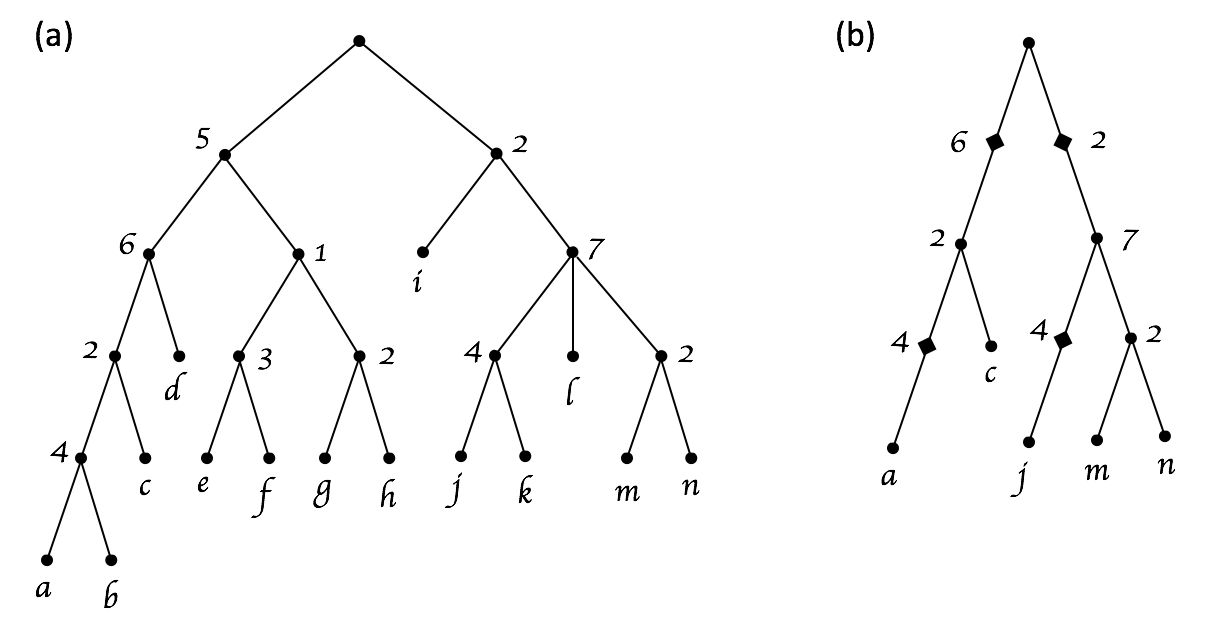
\includegraphics[scale=0.5]{dummynodes}
        \centering
        \caption[Constructing the tree $T||C$]{Part (a) shows a tree $T$ where all internal nodes are labelled with their weights. Part (b) shows the tree $T||C$, where $C = \{a, c, j\}$. Again, internal nodes are labelled with their weights. Nodes represented by diamonds in this figure are dummy nodes. Observe that the dummy node that is two levels above the leaf $c$ has weight $6$ since the nodes on the path from the parent of $c$ to the root of $T$ had weights $6$ and $5$.}
        \label{fig:dummynodes}
    \end{figure}

    Now, we observe some properties of $T||C$. First, we extend the definition $pure$, introduced in Section~\ref{subsec:mincover}, to weighted restricted trees. Let $T||C$ be some tree containing dummy nodes and take any cluster $C' \subseteq C$. Any node $u \in V(T||C)$ belongs to $pure^{T||C}(C')$ iff $u \in V(T)$, $\leafset^{T}(u) \subseteq C'$ and $\leafset^{T}(u) = \leafset^{T||C}(u)$. Thus no dummy node can be pure, which intuitively makes sense, since dummy nodes indicate that some leaves were removed when creating $T||C$ from $T$. Observe that $pure^{T||C}(C') = pure^{T}(C')$, since the pure nodes belong to both $T$ and $T||C$. This also leads to a natural extension of $minCover$ to $T||C$, such that $minCover^{T||C}(C')$ is the set of roots of the subtrees formed by $pure^{T||C}(C')$. Clearly, $minCover^{T||C}(C') = minCover^{T}(C')$.

    Now, we extend the definition of incompatibility to weighted restricted trees. We use the same definition as for normal trees, so that $Conflict^{T||C}(C') = \bigcup_{c \in minCover^{T}(C')} path(c, l_{C'})$, where $l_{C'} = lca^{T||C}(C')$. An important observation to make at this stage is that $max_{u \in Conflict^{T||C}(C')} \weight(u) = max_{u \in Conflict^{T}(C')} \weight(u)$. This is proved below.

    \begin{lemma}
        \label{lem:restrictedweightedmaxincompatible}
        Given a tree $T$ leaf-labelled by $L$ and clusters $C \subseteq L$, $C' \subseteq C$, $max_{u \in Conflict^{T||C}(C')} \weight(u) = max_{u \in Conflict^{T}(C')} \weight(u)$.
    \end{lemma}
        \begin{proof}
            Let $l_{C'} = lca^{T||C}(C')$. Note that $l_{C'} \in V(T)$ since it the $lca$ of some subset of $C$.

            Take any node $u \in Conflict^{T||C}(C')$. Then $u$ is a proper ancestor of some node in $minCover^{T||C}(C')$ and a proper descendant of $l_{C'}$ in $T||C$ by the definition of incompatibility. If $u$ is not a dummy node, then $u \in V(T)$. But $u$ must be a proper ancestor of some node in $minCover^{T}(C')$ and must also be a proper descendant of $l_{C'}$ in $T$. Thus $u \in Conflict^{T}(C')$. If $u$ is a dummy node, then there are some nodes $v, w \in V(T)$ such that $\weight(u) = max_{x \in path^{T}(v, w)} \weight(x)$ and $w = parent^{T||C}(u) = parent^{T||C}(v)$. Since $u \not\in pure^{T||C}(C')$, all nodes in $path^{T}(v, w)$ are proper ancestors of some node in $minCover^{T}(C')$. They must also be proper descendants of $l_{C'}$ in $T$ since $u$ is a proper descendant of $l_{C'}$ in $T||C$. But then $path^{T}(v, w) \subseteq Conflict^{T}(C')$.

            Take any node $u \in Conflict^{T}(C')$. Then $u$ is a proper ancestor of some node in $minCover^{T}(C')$ and a proper descendant of $l_{C'}$ in $T$ by Lemma~\ref{lem:incompatibilitymincover}. If $u$ is the $lca$ of some subset of $C'$ then $u \in V(T||C)$ and clearly $u \in Conflict^{T||C}(C')$. Otherwise, there is some node $v$ which is an ancestor of some node in $minCover^{T}(C')$ and some node $w$ which is a descendant of $l_{C'}$ in $T$ such that $u \in path^{T}(v, w)$ and $w = parent^{T|C}(v)$. Thus, there is some dummy node $z \in V(T||C)$ which represents $path^{T}(v, w)$ and so $\weight(u) \leq \weight(z)$.
        \end{proof}

	Lastly, below lemma show that $T||C$ can be constructed in $O(|C|)$ time.
	\begin{lemma}
		Suppose the lca and the tree rmq data structures of $T_{\beta}$ are given. For any cluster $C$, $T_{\beta}||C$ can be constructed in $O(|C|)$ time.
	\end{lemma}
	\begin{proof}
		First, using lca data structure, we can obtain the tree structure $T_{\beta}|C$ in $O(|C|)$ time. Then, for every node $u$ in $T|C$, we obtain the corresponding weight $\weight(u)$. For every edge $(u, v)$ in $T|C$, we insert a dummy node in between. Its weight is $\max \{ \weight(w) :  w \in path^{T_{\beta}}(u,v) \}$. Using the tree rmq data structure, these weights can be computed in $O(|C|)$ time.
	\end{proof}

%    As part of our algorithm we further restrict already restricted trees. We now show that the $(T||C)||C' = T||C'$.
%    \newline

%    \begin{lemma}
%        \label{lem:furtherrestriction}
%        Given a tree $T$ leaf-labelled by $L$, clusters $C \subseteq L$ and $C' \subseteq C$, $(T||C)||C' = T||C'$.
%    \end{lemma}
%        \begin{proof}
%            We first show that $(T||C)|C' = T|C'$. Recall that $V(T|C') = \{lca^{T}(u, v) : u, v \in C'\}$. Since $C' \subseteq C'$, for any $u, v \in C'$, $u, v \in C$, hence $lca^{T}(u, v) \in V(T||C)$. Further, since dummy nodes only have one child, no dummy node from $T||C$ can be in $(T||C)|C'$. As $T||C$ obeys the same structure as $T$, it must be the case that $(T||C)|C'$ does the same, and hence $(T||C)|C' = T|C'$.
%
%            Now take any $u, v \in V((T||C)|C')$, such that $v = parent^{(T||C)|C'}(u)$ and $path^{T||C}(u, v) \neq \emptyset$. Observe that $u$ and $v$ cannot be dummy nodes, since dummy nodes have only one child and so they cannot be the $lca$ of any cluster. Thus $u, v \in V(T)$. Also, it must be the case that $path^{T}(u, v)$ is non-empty. Further, note that $u, v \in V(T|C')$, since $(T||C)|C' = T|C'$. Thus, we insert a dummy node in both $T||C'$ and $(T||C)||C'$. It is also true that for any $w, w' \in V(T||C)$ where $w$ and $w'$ are not dummy nodes, $rmqTree^{T||C}(w, w') = rmqTree^{T}(w, w')$, since we maintained the maximum weight information in the dummy nodes. Thus the dummy nodes inserted due to $u$ and $v$ in $T||C'$ and $(T||C)||C'$ have the same weights.
%        \end{proof}

    \newpage





    \begin{algorithm}[!ht]
		\caption{FFDCT$(\TA, \TB)$}
        \label{alg:FFDCT}

        \begin{algorithmic}[1]
		\Input Weighted Trees $\TA$, $\TB$.

		\Output ($\mathcal{F}$, $Conflict^{\TB}(\Lambda(\TA))$, $minCover^{\TB}(\leafset^{\TA})$, $lca^{T_{\beta}}(\leafset^{\TA})$) where $\mathcal{F} = \{C \in \mathcal{C}(T_{\alpha}) : \weight(C) > \max_{v \in Conflict^{\TB}(C)} \weight(v) \}$.

		\State {\bf If} $\TA$ is a leaf node $x$, {\bf then} \Return $(\{ x \}, \emptyset, \{ y \}, y)$ where $y$ is the leaf node in $\TB$ with $label(x)=label(y)$
		\State $(\mathcal{F}_{T_{\alpha,hvy}}, Conflict_{T_{\alpha,hvy}}, minCover_{T_{\alpha,hvy}}, \ell_{T_{\alpha,hvy}}) = FFDCT(T_{\alpha,hvy}, \TB)$;
		\For{every subtree $\tau \in sideTree(\TA)$}
		  \State $(\mathcal{F}_{\tau}, Conflict_{\tau}, minCover_{\tau}, \ell_{\tau}) = FFDCT(\tau, \TB||\Lambda(\tau))$;
		\EndFor
		\State $(delNodes, addNodes) = CompCover( minCover_{T_{\alpha,hvy}}, \bigcup_{\tau \in sideTree(\TA)} minCover_{\tau})$
		\label{step:compute-minCover-start}
		\State $minCover = (minCover_{T_{\alpha,hvy}} \cup addNodes) - delNodes$
		\label{step:compute-minCover-end}
		\State Set $Conflict = Conflict_{T_{\alpha,hvy}}$; Set $\ell = lca^{T_{\beta}}( \bigcup_{\tau \in sideTree(\TA)} \{ \ell_{\tau} \} )$
		\label{step:start-Conflict}
		\State Insert ancestors of $addNodes$ which are descendants of $\ell$ to $Conflict$
		\State Insert $path^{T_{\beta}}(\ell_{T_{\alpha,hvy}}, \ell)$ into $Conflict$
		\State Remove nodes $u \in addNodes$ and recurrsively remove the descendants of $u$ in $Conflict$
		\label{step:end-Conflict}
		\State $\mathcal{F} = \bigcup_{\tau \in subTree(\TA)} \mathcal{F}_{\tau}$
		\label{step:start-F}
		\If{$\weight(r(\TA)) >$ maximum weight node in $Conflict$}
                    \label{step:maximumweight}
		    \State $\mathcal{F} = \mathcal{F} \cup \{ \TA \}$
                \EndIf
		\label{step:end-F}
		\State \Return $(\mathcal{F}, Conflict, minCover, \ell)$
        \end{algorithmic}
    \end{algorithm}

    The basic idea of our solution is to collect all clusters $C \in \mathcal{C}(\TA)$ such that $\weight(C) > \max_{C' \in Confict^{\TB}(C)} \weight(C')$.
    Precisely, the algorithm scans all clusters $C \in \mathcal{C}(T_{\alpha})$ and computes $Conflict^{\TB}_{C}$; then, it inserts $C$ in $\mathcal{F}$ if $\weight(C) > \max_{C' \in Confict^{\TB}(C)} \weight(C')$.
    Let $Build(T_{\alpha}, T_{\beta})$ be the function to build


    Below, we assume the lca data structure and the path rmq data structure for $T_{\beta}$ is provided.
    Our algorithm $Filter\_Clusters(T_{\alpha}, T_{\beta})$ is a recursive algorithm (see Algorithm~\ref{alg:FFDCT}).
    It returns four data-structures: (1) $\mathcal{F} = \{ C \in \mathcal{C}(\TA)$ such that $\weight(C) > \max_{C' \in Confict^{\TB}(C)} \weight(C') \}$,
    (2) $\mathcal{I} = Conflict^{\TB}(\Lambda(\TA))$,
    (3) $minCover^{T_{\beta}}(\Lambda(T_{\alpha})$ and (4) $lca^{T_{\beta}}(\Lambda(\TA))$.

    Let $r(T_{\alpha})$ be the root of $T_{\alpha}$. Let $T_{\alpha,hvy}$ be the subtree attached to $r(T_{\alpha})$ which has the most number of leaves.
    Let $sideTree(T_{\alpha})$ be $subTree(T_{\alpha}) - \{ T_{\alpha,hvy} \}$.
    For every subtree $\tau \in sideTree(T_{\alpha})$, the algorithm first recursively calls $Filter\_Clusters(\tau, T_{\beta}||\Lambda(\tau))$.
    For the heavy subtree $T_{\alpha,hvy}$, the algorithm recursively calls $Filter\_Clusters(T_{\alpha,hvy}, T_{\beta})$.
    Then, it computes $minCover$ (Steps~\ref{step:compute-minCover-start}-\ref{step:compute-minCover-end}), $\mathcal{I}$ (Steps~\ref{step:start-Conflict}-\ref{step:end-Conflict}) and $\mathcal{F}$ (Steps~\ref{step:start-F}-\ref{step:end-F}).

    Below lemma gives the time to compute the restricted subtree.
    \begin{lemma}
	    Given the lca data structure and the path rmq data structure for $T_{\beta}$,
	    for any cluster $C$, teh restricted subtree $T_{\beta}||C$ can be computed in $O(|C|)$ time.
    \end{lemma}

    Below lemma give the running time to compute the minimum cover of $T_{\alpha}$.
    Let $Covered(\tau) = \{ v \in V(T_{\beta}) : \Lambda(T_{\beta}[v] \subseteq \Lambda(\tau) \}$.
    \begin{lemma}
	    Consider a tree $T_{\alpha}$ and its corresponding restricted tree $T_{\beta}$. Let $T_{\alpha,hvy}$ be the heavy subtree attached to $r(T)$.
	    For every subtree $\tau \in subTree(T_{\alpha})$, let $minCover_{\tau}$ be the minimum cover of $\tau$.
	    Let $minCover$ be the minimum cover of $T_{\alpha}$
	    Let $addNodes = minCover - minCover_{T_{\alpha,hvy}}$ and $delNodes = minCover_{T_{\alpha,hvy}} - minCover$.
	    $addNodes$ and $delNodes$ can be found in $O(|Covered(T_{\alpha})| - |Covered(T_{\alpha,hvy})|)$ time.
    \end{lemma}

    Given a subtree $\tau$ in $T_{\alpha}$, let $Overlap(\tau) = \{ v \in V(T_{\beta}) : \Lambda(T_{\beta}[v]) \cap \Lambda(\tau) \neq \emptyset \}$.
    Note that $Conflict(\tau) = Overlap(\tau) - Covered(\tau)$.
    Below lemma give the running time to compute $Conflict$.
    \begin{lemma}
	    Consider a tree $T_{\alpha}$ and its corresponding restricted tree $T_{\beta}$. Let $T_{\alpha,hvy}$ be the heavy subtree attached to $r(T)$.
	    For every subtree $\tau \in subTree(T_{\alpha})$, let $minCover_{\tau}$ be the minimum cover of $\tau$.
	    Let $\ell_{\tau}$ be $lca^{T_{\beta}}(\Lambda(\tau))$.
	    Let $minCover$ be the minimum cover of $T_{\alpha}$.
	    Let $addNodes = minCover - minCover_{T_{\alpha,hvy}}$ and $delNodes = minCover_{T_{\alpha,hvy}} - minCover$.
	    Let $Conflict_{T_{\alpha,hvy}}$ be the set of incompatiable nodes in $T_{\beta}$ with respect to $T_{\alpha,hvy}$.
	    Then the set of incompatible nodes in $T_{\beta}$ with respect to $T_{\alpha}$ is $Conflict_{T_{\alpha,hvy}} \cup A \cup B - C$
	    \begin{itemize}
		    \item  $A = path^{T_{\beta}}(\ell_{T_{\alpha,hvy}}, \ell_{T_{\alpha}} ) - Conflict_{T_{\alpha,hvy}}$
		    \item $B = \cup_{u \in addNodes} path^{T_{\beta}}(u, \ell_{T_{\alpha}} ) - Conflict_{T_{\alpha,hvy}}$
		    \item $C = \{ v \in Conflict_{T_{\alpha,hvy}} : v$ is descendant of some $u \in addNodes \}$
	    \end{itemize}
	    $A$ and $B$ can be found in $O(|Overlap(T_{\alpha})| - |Overlap(T_{\alpha,hvy})|)$ time.
	    $C$ can be found in $O(|Covered(T_{\alpha})| - \left( \sum_{\tau \in subtree(T_{\alpha})} |Covered(\tau)| \right) )$ time.
    \end{lemma}

    Hence, we have the following lemma.
    \begin{lemma}
	    $Filter\_Cluster(T_{\alpha})$ runs in $O(n \log n)$ time where $n = |\Lambda(T_{\alpha})|$.
    \end{lemma}


    \newpage


        For any tree $T$ and cluster $C \subseteq \leafset(T)$, define the set $Conflict^{T}(C) = \{u : u \in V(T) \text{ and } \leafset^{T}(u) \not\compatible C\}$. Lemma 6 of \cite{jansson2018algorithms}, which gives a property of this set, is restated here since it is crucial in the development of an algorithm discussed below.
    \newline

    \begin{lemma}
        \label{lem:incompatibility}
        Given a tree $T$ and a cluster $C \subseteq \leafset(T)$, let $l_C = lca^T(C)$. Then for any $u \in V(T)$, $u \in Conflict^{T}(C)$ iff $u$ lies on the path between $l_C$ and some $x \in C$ and $\leafset(u) \not\subseteq C$.
    \end{lemma}


    Section~\ref{subsec:mincover} presents the definition $minCover^{T}(C)$. Section~\ref{subsec:redefiningincompatibility} uses this definition to give a stricter definition of incompatibility. Section~\ref{subsec:restrictedweighted} presents the concept of weighted restricted trees. We then use all of these in Section~\ref{subsec:filterclusters} to create the algorithm \texttt{Filter\_Clusters}. Finally, Sections~\ref{subsec:findcoverer} and~\ref{subsec:updateincompatible} prove two claims we make when analysing the runtime of \texttt{Filter\_Clusters}.

    \subsection{The concepts of pure nodes and covers}
    \label{subsec:mincover}

    Given a tree $T$ leaf-labelled by $L$ and a cluster $C \subseteq L$, define $pure^{T}(C)$ to be the set of nodes $\{u : u \in V(T) \text{ and } \leafset^{T}(u) \subseteq C\}$. Thus for any node $u \in pure^{T}(C)$, the leafset of $u$ contains only leaves from $C$. For example, in Figure~\ref{fig:mincoverrecursive}(a), the circled nodes all belong to $pure^{T}(\{a, b, c, f, g, h\})$.

    We now introduce the related concept of a cover. Define a set $M \subseteq V(T)$ to be a cover of $C$ in $T$ if $\bigcup_{u \in M} \leafset^{T}(u) = C$. Then the minimum cover of $C$ in $T$, denoted as $minCover^{T}(C)$, is the smallest set $M$ such that $M$ is a cover of $C$. Note that this set is well defined for each cluster. For example, in Figure~\ref{fig:mincoverrecursive}(b), the circled nodes give $minCover^{T}(\{a, b, c, f, g, h\})$. Observe that the subtrees rooted at nodes in the minimum cover give exactly the set of pure nodes, i.e. $\bigcup_{u \in minCover^{T}(C)} V(T[u]) = pure^{T}(C)$.

    Finally, for any node $u \in V(T)$ such that $\leafset^{T}(u) \subseteq C$, define the node covering $u$, denoted as $coverer^{T, C}(u)$, to be the ancestor of $u$ which belongs to $minCover^{T}(C)$. Observe that this node must exist, since $\leafset^{T}(u)$ must be covered, and covering it with descendants of $u$ certainly yields a larger cover than if we use $u$. Again referring to Figure~\ref{fig:mincoverrecursive}(b), let $C = \{a, b, c, f, g, h\}$, then $coverer^{T, C}(u) = v$.

    \begin{figure}[ht]
        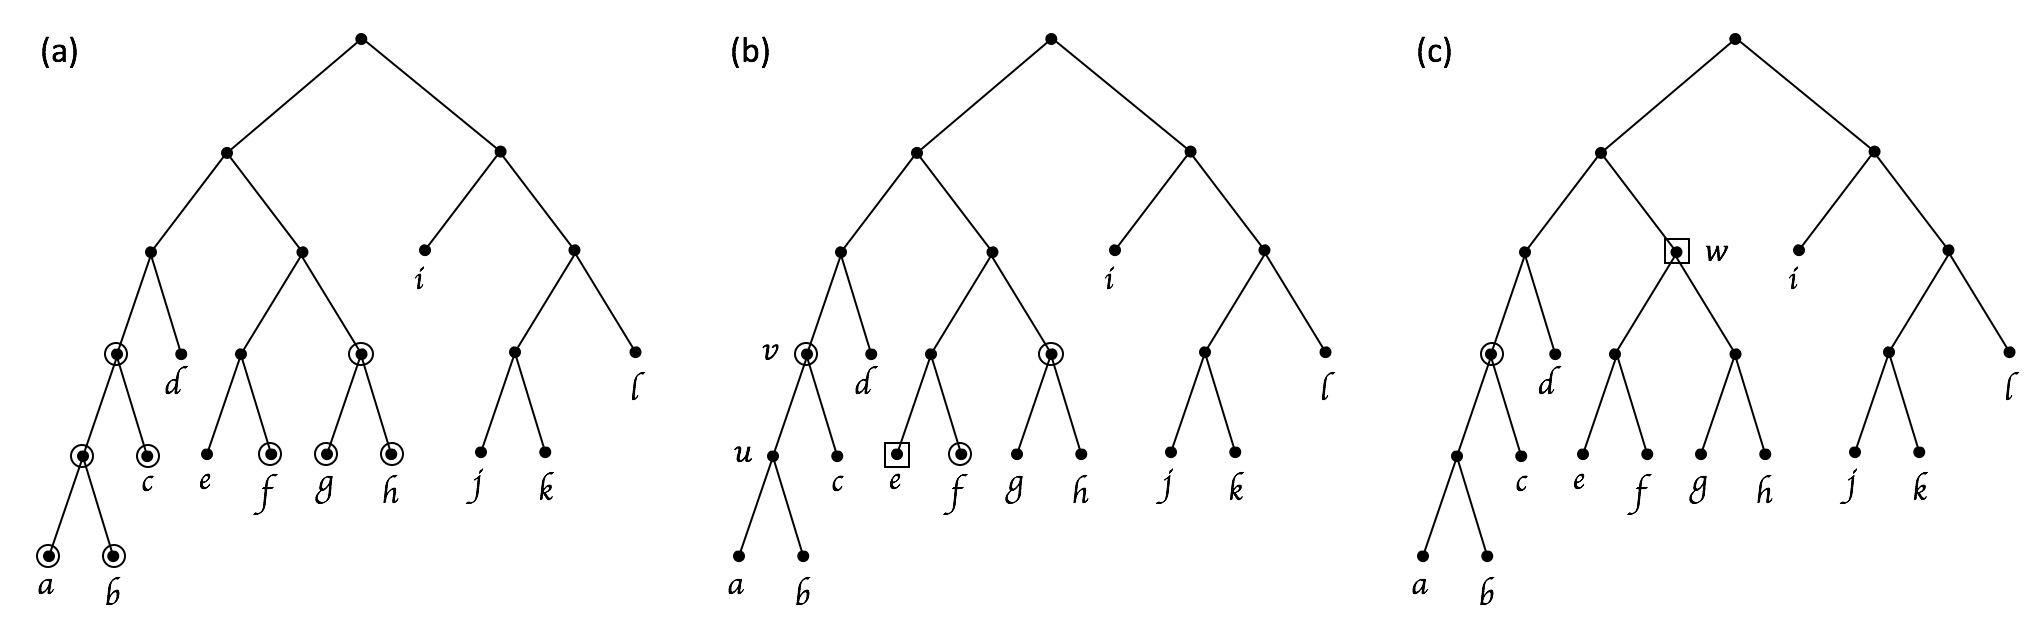
\includegraphics[width=\textwidth]{mincoverrecursive}
        \centering
        \caption[Pure nodes and covers]{Illustration of the concepts of pure nodes and covers. Let $C = \{a, b, c, f, g, h\}$. Then the circled nodes in (a) give $pure^{T}(C)$. The circled nodes in (b) give $minCover^{T}(C)$. In (b), $coverer^{T, C}(u) = v$. Take the leaf $e$, marked with a square in (b) and let $Ce = C \cup \{e\}$. Then $coverer^{T, Ce}(e) = w$, marked with a square in (c). Then the circled node and $w$ in (c) give $minCover^{T}(Ce)$.}
        \label{fig:mincoverrecursive}
    \end{figure}

    Given some tree $T$ leaf-labelled by $L$, cluster $C \subseteq L$ and node $u \in V(T)$ such that $\leafset^{T}(u) \cap C = \emptyset$, let $M = minCover^{T}(C)$ and $Cu = C \cup \leafset^{T}(u)$. Then it is useful to be able to find $coverer^{T, Cu}(u)$. Thus, we define the operation $findCoverer^{T, Cu}(u)$ which returns $coverer^{T, Cu}(u)$.

    Figure~\ref{fig:mincoverrecursive} demonstrates how this query works. Here, $C = \{a, b, c, f, g, h\}$ and we take the leaf $e$. The circled nodes in Figure~\ref{fig:mincoverrecursive}(b) give $minCover^{T}(C)$. Then we wish to compute $coverer^{T, Ce}(e)$, where $Ce = C \cup \{e\}$. The idea for doing so will be to iterate upwards from $e$ while the leafset of the node we are at is a subset of $Ce$. Thus, since $\leafset^{T}(parent(e)) \subseteq Ce$, we go upwards one level. We can then go a further  level, to the node $w$ since $\leafset^{T}(w) \subseteq Ce$. At this point we cannot go any further up. Hence, we say that we have found $w = coverer^{T, Ce}(e)$. This yields the following definition of $findCoverer^{T, Cu}(u)$:
    \newline

    \begin{lemma}
        \label{lem:findcovererrecursive}
        Given a tree $T$ leaf-labelled by $L$, a cluster $C \subseteq L$ and a node $u \in V(T)$ such that $\leafset^{T}(u) \cap C = \emptyset$, let $M = minCover^{T}(C)$, $Cu = C \cup \leafset^{T}(u)$ and $v = parent(u)$. Then
        \[findCoverer^{T, Cu}(u) = \begin{cases}
            u & \leafset^{T}(v) \not\subseteq Cu\\
            findCoverer^{T, Cu}(v) & otherwise
        \end{cases}\]
    \end{lemma}
        \begin{proof}
            \textit{Base Case.} If $\leafset^{T}(v) \not\subseteq Cu$, there is some leaf $x \in \leafset^{T}(v)$ such that $x \not\in C$. Thus $v$ cannot cover $\leafset^{T}(u)$, so $u = coverer^{T, Cu}(u)$.

            \textit{Inductive Case.} Since $v = parent(u)$ and $\leafset^{T}(v) \subseteq Cu$, $coverer^{T, Cu}(u) = coverer^{T, Cu}(v)$ so the algorithm works recursively. Also observe that the recursion has to terminate since in each recursive call we go one node further up the tree.
        \end{proof}

    Now given $coverer^{T, Cu}(u)$, we would like to actually obtain the minimum cover of $Cu$. Referring back to Figure~\ref{fig:mincoverrecursive}, notice that we can subtract the set of all children of the nodes on the path from $e$ to $w$ (excluding $e$) from $M$, add $w$, and this gives us the required set. That is, we take $M \cup \{w\} - \bigcup_{w' \in path^{T}(e, w]} children(w')$. This leads to the following lemma:
    \newline

    \begin{lemma}
        \label{lem:mincoverrecursive}
        Given a tree $T$ leaf-labelled by $L$, a cluster $C \subseteq L$ and a node $u \in V(T)$ such that $\leafset^{T}(u) \cap C = \emptyset$ let $M = minCover^{T}(C)$, $Cu = C \cup \leafset^{T}(u)$ and $v = coverer^{T, Cu}(u)$. Then
         \[minCover^{T}(Cu) = M \cup \{v\} - \bigcup_{w \in path^{T}(u, v]} children(w)\]
    \end{lemma}
        \begin{proof}
            Firstly, $M \cup \{v\} - \bigcup_{w \in path^{T}(u, v]} children(w)$ covers $Cu$. To see this, take any leaf $x \in Cu$. Then if $x \in \leafset^{T}(v)$, then we are clearly done. Otherwise, $x \in C$, so there must be some $c \in M$ such that $x \in leafset^{T}(c)$. But $c \not\in \bigcup_{w \in path^{T}(u, v]} children(w)$, otherwise $x \in \leafset^{T}(v)$. Thus $c \in M - \bigcup_{w \in path^{T}(u, v]} children(w)$, so we are done.

            Further, this must also be the minimum cover of $Cu$. Clearly, $v$ provides the smallest cover for $\leafset^{T}(v)$, which encapsulates $\leafset^{T}(u)$. Then if there is a smaller cover for $Cu$, we can cut and paste this into $M$, giving a smaller cover for $C$, which contradicts the definition of $M$.

            Thus we have the minimum cover for $Cu$.
        \end{proof}

    Section~\ref{subsec:findcoverer} details how to actually implement the \texttt{Find\_Coverer} operation. We now make a claim (proved later) about its running time.
    \newline

    \begin{lemma}
        \label{lem:findcovererruntime}
        Given a tree $T$ leaf-labelled by $L$, a cluster $C \subseteq L$ and a node $u \in V(T)$ such that $\leafset^{T}(u) \cap C = \emptyset$, let $M = minCover^{T}(C)$, $Cu = C \cup \leafset^{T}(u)$ and $v = coverer^{T, Cu}(u)$. Then the operations $findCoverer^{T, Cu}(u)$ can be performed in $O(|path^{T}(u, v]| + 1)$ time.
    \end{lemma}
        \begin{proof}
            Proved in Section~\ref{subsec:findcoverer}.
        \end{proof}

    \subsection{Redefining incompatibility}
    \label{subsec:redefiningincompatibility}

    With the concept of a minimum cover in hand, we can proceed to give a method to compute incompatibility. Given a tree $T$ and a cluster $C \subseteq L$, recall that the set $Conflict^{T}(C) = \{v : v \in V(T) \text{ and } \leafset^{T}(v) \not\compatible C\}$.
    \newline

    \begin{lemma}
        \label{lem:incompatibilitymincover}
        Given a tree $T$ leaf-labelled by $L$ and a cluster $C \subseteq L$, let $l_C = lca^{T}(C)$. Then for any node $u \in V(\TB)$, $u \in Conflict^{T}(C)$ iff $u$ is a proper ancestor of some node $c \in minCover^{T}(C)$ and $u$ is a proper descendant of $l_C$. In other words, $Conflict^{T}(C) = \bigcup_{c \in minCover^{T}(C)} path(c, l_C)$.
    \end{lemma}
        \begin{proof}
		($\longrightarrow$) Given any $u \in V(T)$ such that $u \in Conflict^{T}(C)$, $u$ is a proper descendant of $l_C$ as a direct consequence of Lemma~\ref{lem:incompatibility}. Further, there is some leaf $x \in C$ such that $u$ is a proper ancestor of $x$ by Lemma~\ref{lem:incompatibility}. Then there must be some node $c \in V(T)$ such that $c$ is an ancestor of $x$ and $c \in minCover^{T}(C)$, otherwise $x$ would not be covered. If $c$ is an ancestor of $u$, then $\leafset^{T}(u) \subseteq \leafset^{T}(c) \subseteq C$, thus $\leafset^{T}(u) \compatible C$, which leads to a contradiction. Hence, $u$ is a proper ancestor of $c$.

		($\longleftarrow$) Given any $u \in V(T)$ such that $u$ is a proper ancestor of some node $c \in minCover^{T}(C)$ and $u$ is a proper descendant of $l_C$, $C \not\subseteq \leafset^{T}(u)$, since $u$ is a proper descendant of $l_C$. As $u$ is a proper ancestor of $c$, $\leafset^{T}(c) \subset \leafset^{T}(u)$. Also, $\leafset^{T}(c) \subset C$ by the definition of minimum cover. Thus $\leafset^{T}(u) \cap C \neq \emptyset$. Also, if $\leafset^{T}(u) \subseteq C$, we could create a smaller cover for $C$ by removing all proper descendants of $u$ from $minCover^{T}(C)$ and adding $u$. Note that this would give a smaller cover as there must be more than one such proper descendant of $u$, since $c$ is a proper descendant of $u$ and $\leafset^{T}(c) \subset C$. Hence, $u \in Conflict^{T}(C)$.
        \end{proof}

    The above result is illustrated in Figure~\ref{fig:incompatibility}(a).

    \begin{figure}[ht]
        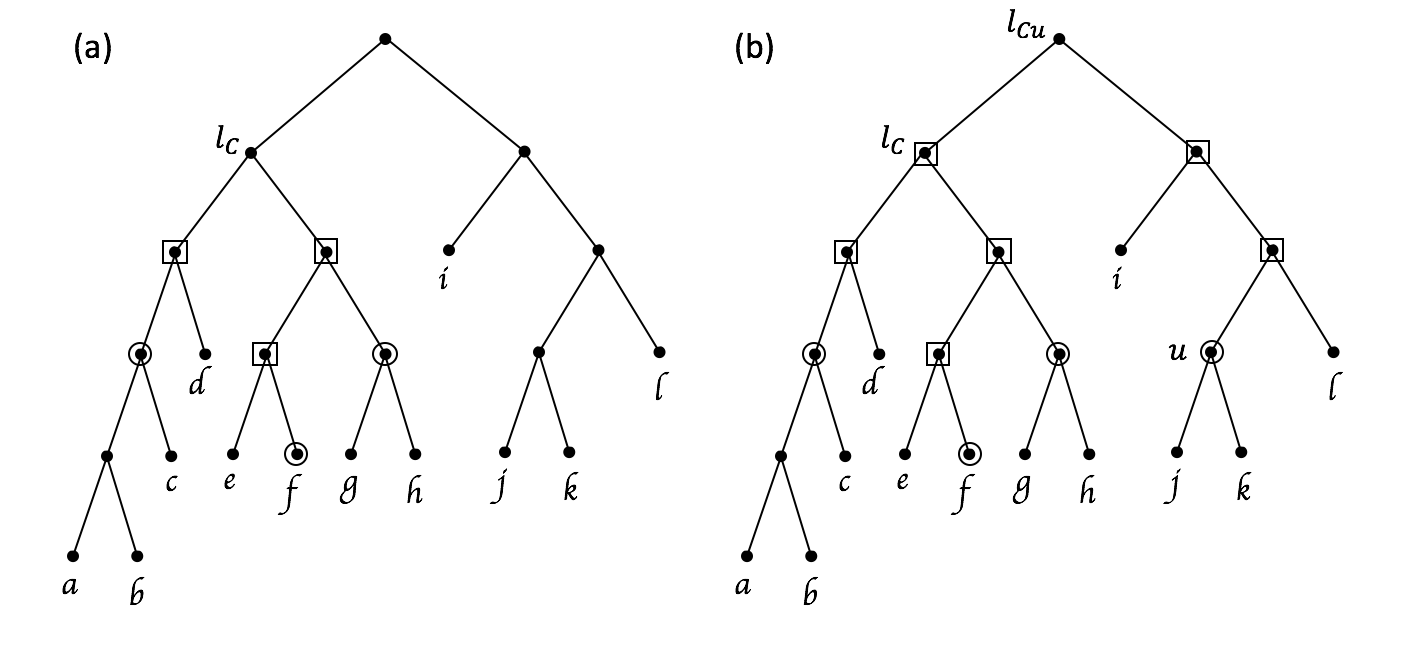
\includegraphics[scale=0.5]{incompatibility}
        \centering
        \caption[Incompatibility and the $updateIncompatible$ operation]{Illustration of Lemma~\ref{lem:incompatibilitymincover} and an $updateIncompatible$ operation. Let $C = \{a, b, c, f, g, h\}$. Then in (a), $l_C = lca^T(C)$, the circled nodes give $minCover^{T}(C)$ and the nodes marked with squares give $Conflict^T(C)$. Notice that all nodes in $Conflict^T(C)$ are proper descendants of $l_C$ and proper ancestors of some $c \in minCover^{T}(C)$. Referencing (b), let $Cu = C \cup \leafset^{T}(u)$ and $l_{Cu} = lca^{T}(Cu)$. Note that $u = coverer^{T, Cu}(u)$. Then we run $updateIncompatible^{T}(Conflict^{T}(C), u, u, l_C, l_{Cu})$. Again, nodes in $minCover^{T}(Cu)$ are circled and nodes in $Conflict^{T}(Cu)$ are marked with squares.}
        \label{fig:incompatibility}
    \end{figure}

    We now wish to define an operation which takes the set of nodes incompatible with a given cluster and updates this set to become those incompatible with a superset of that cluster. Formally, given tree a $T$ leaf-labelled by $L$, a cluster $C \subseteq L$ and a node $u \in V(T)$ such that $\leafset^{T}(u) \cap C = \emptyset$, we would like to have an operation that takes in $I$ and $u$ (along with some other arguments) and returns $Conflict^{T}(C \cup \leafset^{T}(u))$. Figure~\ref{fig:incompatibility}(b) shows the result of an $updateIncompatible$ query.

    \begin{figure}[ht]
        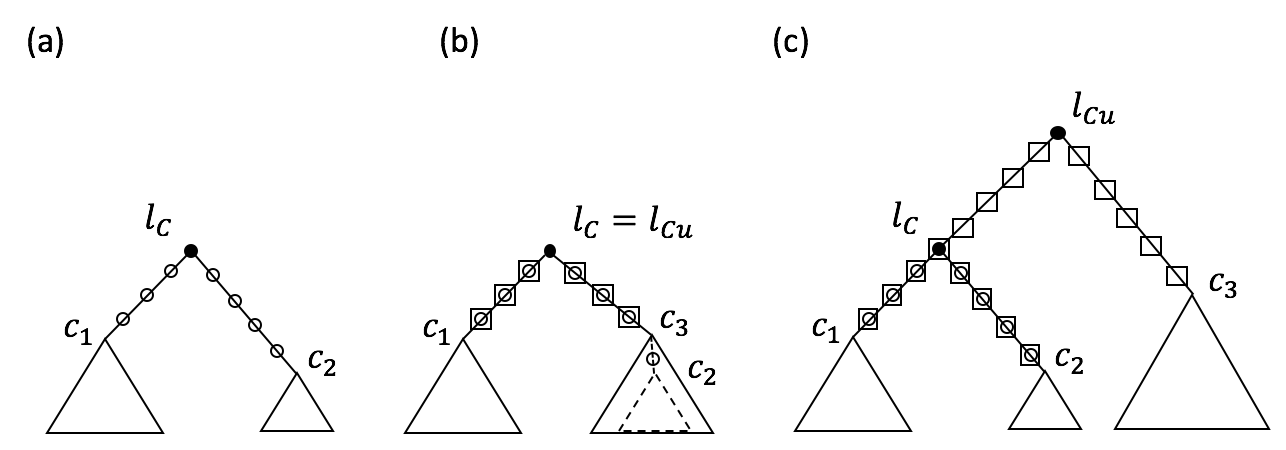
\includegraphics[scale=0.6]{incompatibilityrecursive}
        \centering
        \caption[Recursively defining incompatibility]{Illustration of a recursive definition of incompatibility. Let $minCover^{T}(C) = \{c_1, c_2\}$ and circled nodes be in $Conflict^{T}(C)$, as in (a). For some node $u \in V(T)$, let $Cu = C \cup \leafset^{T}(u)$ and the nodes $l_C$ and $l_{Cu}$ be $lca^{T}(C)$ and $lca^{T}(Cu)$ respectively. In (b), $minCover^{T}(Cu) = \{c_1, c_3\}$, and $l_C = l_{Cu}$, while in (c), $minCover^{T}(Cu) = \{c_1, c_2, c_3\}$ and $l_C \neq l_{Cu}$. In both (b) and (c), nodes belonging to $Conflict^{T}(Cu)$ are marked with squares and $coverer^{T, Cu}(u) = c_3$.}
        \label{fig:incompatibilityrecursive}
    \end{figure}

    We use observations from Figure~\ref{fig:incompatibilityrecursive} to gain intuition that helps us develop this operation. Let $minCover^{T}(C) = \{c_1, c_2\}$ and circled nodes belong to $Conflict^{T}(C)$, as shown in Figure~\ref{fig:incompatibilityrecursive}(a). For some node $u \in V(T)$, let $Cu = C \cup \leafset^{T}(u)$ and the nodes $l_C$ and $l_{Cu}$ be $lca^{T}(C)$ and $lca^{T}(Cu)$ respectively. Then Figure~\ref{fig:incompatibilityrecursive}(b) gives a case where $minCover^{T}(Cu) = \{c_1, c_3\}$. Here, $l_C = l_{Cu}$. Nodes in $Conflict^{T}(Cu)$ are marked with squares. Observe that the nodes in $path^{T}(c_2, c_3] = path^{T}(c_2, coverer^{T, Cu}(u)]$ belonged to $Conflict^{T}(C)$ but do not belong to $Conflict^{T}(Cu)$. The case where $minCover^{T}(Cu) = \{c_1, c_2, c_3\}$ and $l_C \neq l_{Cu}$ is shown in Figure~\ref{fig:incompatibilityrecursive}(c). In this case, we have to add the nodes in $path^{T}(c_3, l_{Cu}) = path^{T}(coverer^{T, Cu}(u), l_{Cu})$ and $path^{T}(l_C, l_{Cu})$ to $Conflict^{T}(C)$ to get $Conflict^{T}(Cu)$. We need to be a little careful with adding $l_C$ to $Conflict^{T}(C)$ though. Firstly, if $\leafset^{T}(l_C) = C$, then $\leafset^{T}(l_C) \subseteq Cu$, so it should not be added. However, if $\leafset^{T}(l_C) \neq C$ (and $l_C \neq l_{Cu}$) then it should be added. These observations are encapsulated in the following Lemma.
    \newline

    \begin{lemma}
        \label{lem:incompatibilityrecursive}
        Given a tree $T$ leaf-labelled by $L$, a cluster $C \subseteq L$ and a node $u \in V(T)$ such that $\leafset^{T}(u) \cap C = \emptyset$, let $I = Conflict^{T}(C)$, $Cu = C \cup \leafset^{T}(u)$, $v = coverer^{T, Cu}(u)$, $l_C = lca^{T}(C)$ and $l_{Cu} = lca^{T}(Cu)$. Then $Conflict^{T}(Cu)$ can be defined as follows
        \begin{align*}
            Conflict^{T}(Cu) = &(I - path^{T}(u, v]) \cup path^{T}(v, l_{Cu}) \cup path^{T}(l_C, l_{Cu}) \cup
            \begin{cases}
                \{l_C\} & \leafset^{T}(l_C) \neq C \text{ and } l_C \neq l_{Cu}\\
                \emptyset & otherwise
            \end{cases}
        \end{align*}
    \end{lemma}
        \begin{proof}
            By Lemma~\ref{lem:mincoverrecursive}, $minCover^{T}(Cu) - minCover^{T}(C) = \{v\}$ and $minCover(C) - minCover^{T}(Cu) \subseteq V(T[v])$. We represent the RHS of the equation in the Lemma by $X$.

		($\longrightarrow$) Take any node $w \in X$.

            Take the case where $w \in I - path^{T}(u, v]$. Since $w \in I$, there is some $c \in minCover^{T}(C)$ such that $w \in path^{T}(c, l_{C})$, by Lemma~\ref{lem:incompatibilitymincover}. If $c \not\in V(T[v])$, then $c \in minCover^{T}(Cu)$ and so $w \in Conflict^{T}(Cu)$. Otherwise, $c \in V(T[v])$. If $w$ is a proper ancestor of $v$, then $w \in Conflict^{T}(Cu)$. Otherwise, $w \in V(T[v])$. Since $w \in I - path^{T}(u, v]$, $w \not\in path^{T}(u, v]$, so $w$ is not an ancestor of $u$. Since $w \in Conflict^{T}(C)$, there is some leaf $x \in \leafset^{T}(w)$ such that $x \not\in C$. But also $x \not\in \leafset^{T}(u)$. Then $v \not\in minCover^{T}(Cu)$ because $x \in \leafset^{T}(v)$, which gives a contradiction, hence $w \not\in V(T[v])$.

            Otherwise, if $w \in path^{T}(v, l_{Cu})$, then $w \in Conflict^{T}(Cu)$ by Lemma~\ref{lem:incompatibilitymincover}.

            Otherwise, suppose $w \in path^{T}(l_C, l_{Cu})$. Then $C \subset \leafset^{T}(w)$. Also, $v$ is not a descendant of $w$, otherwise $w = l_{Cu}$. So $Cu - \leafset^{T}(w) \neq \emptyset$. Since $C \subset \leafset^{T}(w)$, there is some leaf $x \in \leafset^{T}(w)$ such that $x \not\in C$. Also, $x \not\in \leafset^{T}(u)$ since $v$ is not a descendant of $w$, so $x \not\in Cu$. Finally, $\leafset^{T}(w) \cap Cu \neq \emptyset$ because $C \subset \leafset^{T}(w)$ and $C \subset Cu$, thus $w \in Conflict^{T}(Cu)$.

            If none of the above are true, $w = l_C$ and $\leafset^{T}(l_C) \neq C$ and $l_C \neq l_{Cu}$. Clearly $\leafset^{T}(l_C) \cap Cu \neq \emptyset$. Since $\leafset^{T}(l_C) \neq C$, there is some leaf $x \in \leafset^{T}(l_C)$ such that $x \not\in C$. But also $x \not\in \leafset^{T}(u)$, other $l_C = l_{Cu}$. Thus $x \not\in Cu$, so $\leafset^{T}(l_C) \not\subseteq Cu$. Finally, $Cu \not\subseteq \leafset^{T}(l_C)$, since $l_C \neq l_{Cu}$. Thus $w \in Conflict^{T}(Cu)$.

		($\longrightarrow$) Take any node $w \in Conflict^{T}(Cu)$.

            By Lemma~\ref{lem:incompatibilitymincover}, there is some $c \in minCover^{T}(Cu)$ such that $w \in path^{T}(c, l_{Cu})$. If $c = v$, then $w \in X$. Otherwise, $c \in minCover^{T}(C)$ since $minCover^{T}(Cu) - minCover^{T}(C) = \{v\}$. If $w$ is a proper descendant of $l_C$, then $w \in I - path^{T}(u, v]$ by Lemma~\ref{lem:incompatibilitymincover}. If $w = l_C$, then $\leafset^{T}(l_C) \neq C$, otherwise $\leafset^{T}(l_C) \compatible Cu$. Also, $l_C \neq l_{Cu}$, since $l_{Cu} \not\in Conflict^{T}(Cu)$, so $w \in X$. Finally, if $w$ is a proper ancestor of $l_C$, then $w \in path^{T}(l_C, l_{Cu})$, so $w \in X$.
        \end{proof}

    Thus we define the operation $updateIncompatible^{T}(I, u, v, l_C, l_{Cu})$ which returns $Conflict^{T}(Cu)$. The actual implementation of this operation is detailed in Section~\ref{subsec:updateincompatible}. We now make a claim about the running time of the $updateIncompatible$ operation, which is proved later.
    \newline

    \begin{lemma}
        \label{lem:updateincompatibleruntime}
        Given a tree $T$ leaf-labelled by $L$, a cluster $C \subseteq L$ and a node $u \in V(T)$ such that $\leafset^{T}(u) \cap C = \emptyset$, let $I = Conflict^{T}(C)$, $Cu = C \cup \leafset^{T}(u)$, $l_C = lca^{T}(C)$, $l_{Cu} = lca^{T}(Cu)$ and $v = coverer^{T, Cu}(u)$. Let $removed$ be the set of nodes deleted from $I$ when calling $updateIncompatible^{T}(I, u, v, l_C, l_{Cu})$ and $added$ be the set of nodes inserted into $I$. Then the operation can be performed in $O(|added| + |removed|\,\times\,log\,n + 1)$ time, where $n = |\leafset^{T}|$.
    \end{lemma}
        \begin{proof}
            Proved in Section~\ref{subsec:updateincompatible}.
        \end{proof}

    Note that the $log\,n$ factor comes about due to the data structure used to store $I$; this is explained in detail later.

    \subsection{Weighted Restricted Trees}
    \label{subsec:restrictedweighted}

    Recall the concept of restricted trees introduced in Section~\ref{subsec:restrictedtree} - given a tree $T$ leaf-labelled by $L$ and a cluster $C \subseteq L$, $V(T|C) = \{lca^T(u, v) : u, v \in C\}$ which obeys $lca^T(C') = lca^{T|C}(C')$ for all clusters $C' \subseteq C$. Observe that certain nodes are deleted from $T$ when forming $T|C$; this leads to losing information about the weights of these nodes. Hence, we extend the concept of restricted trees to the case where the tree is weighted, following the definition given in \cite{jansson2018algorithms}.

    Given a tree $T$ leaf-labelled by $L$, a cluster $C \subseteq L$ and for each node $u \in V(T)$, the value $\weight(u)$, we define the tree $T||C$, read as ``weighted $T$ restricted to $C$''. First, the tree $T|C$ is constructed and let the weight of each node in this tree be the same as its weight in $T$. Now for each non-root node $u \in V(T|C)$, let $v = parent^{T|C}(u)$. Then if $path^{T}(u, v) \neq \emptyset$ we create a dummy node $z$ in $T|C$ and set $parent(u) = z$ and $parent(z) = v$. Also, $\weight(z)$ is set as $rmqTree^{T}(u, v)$. Intuitively, if $path^{T}(u, v) \neq \emptyset$, then the nodes in this path have been deleted from $T$ to form $T|C$. As we wish to retain some information about their weights, we insert the dummy node $z$ into $T||C$ to represent this path and hold the largest weight along it. Figure~\ref{fig:dummynodes} demonstrates this procedure.

    \begin{figure}[ht]
        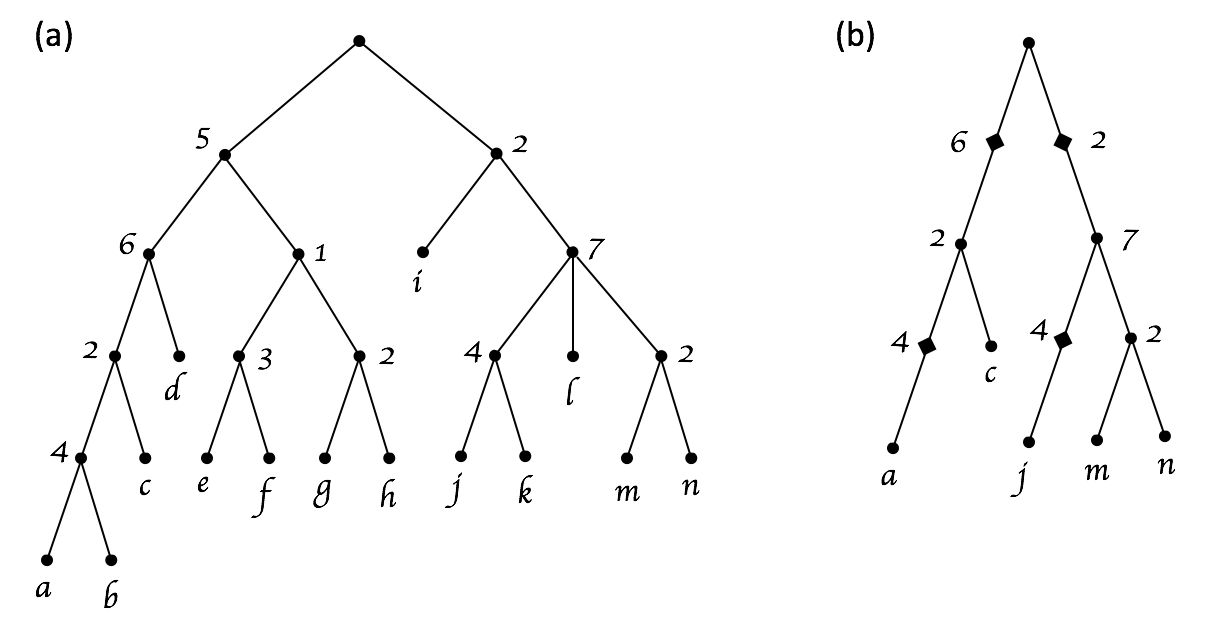
\includegraphics[scale=0.5]{dummynodes}
        \centering
        \caption[Constructing the tree $T||C$]{Part (a) shows a tree $T$ where all internal nodes are labelled with their weights. Part (b) shows the tree $T||C$, where $C = \{a, c, j\}$. Again, internal nodes are labelled with their weights. Nodes represented by diamonds in this figure are dummy nodes. Observe that the dummy node that is two levels above the leaf $c$ has weight $6$ since the nodes on the path from the parent of $c$ to the root of $T$ had weights $6$ and $5$.}
        \label{fig:dummynodes}
    \end{figure}

    Now, we observe some properties of $T||C$. First, we extend the definition $pure$, introduced in Section~\ref{subsec:mincover}, to weighted restricted trees. Let $T||C$ be some tree containing dummy nodes and take any cluster $C' \subseteq C$. Any node $u \in V(T||C)$ belongs to $pure^{T||C}(C')$ iff $u \in V(T)$, $\leafset^{T}(u) \subseteq C'$ and $\leafset^{T}(u) = \leafset^{T||C}(u)$. Thus no dummy node can be pure, which intuitively makes sense, since dummy nodes indicate that some leaves were removed when creating $T||C$ from $T$. Observe that $pure^{T||C}(C') = pure^{T}(C')$, since the pure nodes belong to both $T$ and $T||C$. This also leads to a natural extension of $minCover$ to $T||C$, such that $minCover^{T||C}(C')$ is the set of roots of the subtrees formed by $pure^{T||C}(C')$. Clearly, $minCover^{T||C}(C') = minCover^{T}(C')$.

    Now, we extend the definition of incompatibility to weighted restricted trees. We use the same definition as for normal trees, so that $Conflict^{T||C}(C') = \bigcup_{c \in minCover^{T}(C')} path(c, l_{C'})$, where $l_{C'} = lca^{T||C}(C')$. An important observation to make at this stage is that $max_{u \in Conflict^{T||C}(C')} \weight(u) = max_{u \in Conflict^{T}(C')} \weight(u)$. This is proved below.

    \begin{lemma}
        \label{lem:restrictedweightedmaxincompatible}
        Given a tree $T$ leaf-labelled by $L$ and clusters $C \subseteq L$, $C' \subseteq C$, $max_{u \in Conflict^{T||C}(C')} \weight(u) = max_{u \in Conflict^{T}(C')} \weight(u)$.
    \end{lemma}
        \begin{proof}
            Let $l_{C'} = lca^{T||C}(C')$. Note that $l_{C'} \in V(T)$ since it the $lca$ of some subset of $C$.

            Take any node $u \in Conflict^{T||C}(C')$. Then $u$ is a proper ancestor of some node in $minCover^{T||C}(C')$ and a proper descendant of $l_{C'}$ in $T||C$ by the definition of incompatibility. If $u$ is not a dummy node, then $u \in V(T)$. But $u$ must be a proper ancestor of some node in $minCover^{T}(C')$ and must also be a proper descendant of $l_{C'}$ in $T$. Thus $u \in Conflict^{T}(C')$. If $u$ is a dummy node, then there are some nodes $v, w \in V(T)$ such that $\weight(u) = max_{x \in path^{T}(v, w)} \weight(x)$ and $w = parent^{T||C}(u) = parent^{T||C}(v)$. Since $u \not\in pure^{T||C}(C')$, all nodes in $path^{T}(v, w)$ are proper ancestors of some node in $minCover^{T}(C')$. They must also be proper descendants of $l_{C'}$ in $T$ since $u$ is a proper descendant of $l_{C'}$ in $T||C$. But then $path^{T}(v, w) \subseteq Conflict^{T}(C')$.

            Take any node $u \in Conflict^{T}(C')$. Then $u$ is a proper ancestor of some node in $minCover^{T}(C')$ and a proper descendant of $l_{C'}$ in $T$ by Lemma~\ref{lem:incompatibilitymincover}. If $u$ is the $lca$ of some subset of $C'$ then $u \in V(T||C)$ and clearly $u \in Conflict^{T||C}(C')$. Otherwise, there is some node $v$ which is an ancestor of some node in $minCover^{T}(C')$ and some node $w$ which is a descendant of $l_{C'}$ in $T$ such that $u \in path^{T}(v, w)$ and $w = parent^{T|C}(v)$. Thus, there is some dummy node $z \in V(T||C)$ which represents $path^{T}(v, w)$ and so $\weight(u) \leq \weight(z)$.
        \end{proof}

    As part of our algorithm we further restrict already restricted trees. We now show that the $(T||C)||C' = T||C'$.
    \newline

    \begin{lemma}
        \label{lem:furtherrestriction}
        Given a tree $T$ leaf-labelled by $L$, clusters $C \subseteq L$ and $C' \subseteq C$, $(T||C)||C' = T||C'$.
    \end{lemma}
        \begin{proof}
            We first show that $(T||C)|C' = T|C'$. Recall that $V(T|C') = \{lca^{T}(u, v) : u, v \in C'\}$. Since $C' \subseteq C'$, for any $u, v \in C'$, $u, v \in C$, hence $lca^{T}(u, v) \in V(T||C)$. Further, since dummy nodes only have one child, no dummy node from $T||C$ can be in $(T||C)|C'$. As $T||C$ obeys the same structure as $T$, it must be the case that $(T||C)|C'$ does the same, and hence $(T||C)|C' = T|C'$.

            Now take any $u, v \in V((T||C)|C')$, such that $v = parent^{(T||C)|C'}(u)$ and $path^{T||C}(u, v) \neq \emptyset$. Observe that $u$ and $v$ cannot be dummy nodes, since dummy nodes have only one child and so they cannot be the $lca$ of any cluster. Thus $u, v \in V(T)$. Also, it must be the case that $path^{T}(u, v)$ is non-empty. Further, note that $u, v \in V(T|C')$, since $(T||C)|C' = T|C'$. Thus, we insert a dummy node in both $T||C'$ and $(T||C)||C'$. It is also true that for any $w, w' \in V(T||C)$ where $w$ and $w'$ are not dummy nodes, $rmqTree^{T||C}(w, w') = rmqTree^{T}(w, w')$, since we maintained the maximum weight information in the dummy nodes. Thus the dummy nodes inserted due to $u$ and $v$ in $T||C'$ and $(T||C)||C'$ have the same weights.
        \end{proof}

    Observe that, as shown in the proof for Lemma~\ref{lem:furtherrestriction}, when constructing $(T||C)||C'$, we can actually make the $rmqTree$ queries against $T$ instead $T||C$. Thus we use an $rmqTree$ structure constructed on the original $T$ for all subsequent restrictions.

    \subsection{The \texttt{Filter\_Clusters} algorithm}
    \label{subsec:filterclusters}

    We redefine \texttt{Filter\_Clusters} to take trees $\TA$ and $\TB$ where $\leafset^{\TA} = \leafset^{\TB} = L$ and return a representation of the cluster collection $\{C : C \in \mathcal{C}(\TA) \text{ and } \weight(C) > max(\{\weight(C_1) : C_1 \in \mathcal{C}(\TB) \text{ and } C_1 \not\compatible C\})\}$. This obeys the original definition when $\TB$ is not a weighted restricted tree, since the root of $\TA$ will be compatible with $\TB$ and so we can represent the above cluster collection as a tree $T$.

    However, if $\TB$ is a weighted restricted tree, then the root of $\TA$ may actually be incompatible with some nodes in $\TB$, as given by the definition of incompatibility for weighted restricted trees. Then this cluster may not be in the final cluster collection, and hence we represent the output with a forest $\mathcal{F}$, such that the overall cluster collection of the trees in the forest, i.e. $\bigcup_{T \in \mathcal{F}} \mathcal{C}(T)$, gives us the set we need. Observe that, given trees $\tau$ and $\TB$ such that $\leafset^{\tau} \subseteq \leafset^{\TB} = L$ and $\TB$ is not a weighted restricted tree, \texttt{Filter\_Clusters}$(\tau, \TB||\leafset^{\tau})$ returns the cluster collection $\{C : C \in \mathcal{C}(\tau) \text{ and } \weight(C) > max(\{\weight(C_1) : C_1 \in \mathcal{C}(\TB) \text{ and } C_1 \not\compatible C\})\}$, due to Lemma~\ref{lem:restrictedweightedmaxincompatible}. That is, calling \texttt{Filter\_Clusters} on the weighted restricted tree actually gives the clusters in $\tau$ that obey the frequency difference condition with respect to $\TB$ and not $\TB||\leafset^{\tau}$.

    Finally, for any node $u \in V(\TA)$, define $Conflict^{\TB}(u)$ to be $Conflict^{\TB}(\leafset^{\TA}(u))$. As discussed earlier, the idea is to find the maximum weight of any node in $Conflict^{\TB}(u)$ for each node $u \in V(\TA)$.

    Algorithm~\ref{alg:filterclusters} gives the algorithm \texttt{Filter\_Clusters}. Step~\ref{step:centroidpath} decomposes $\TA$ into a \textit{centroid path} $\langle p_{\gamma}, p_{\gamma - 1}, \dots, p_1 \rangle$, where $p_{\gamma}$ is the root of $\TA$, and a set of \textit{side trees} (similarly to \cite{jansson2018algorithms}). Observe that for any side tree $\tau \in \sigma(\TA)$, $|\leafset^\tau| \leq n/2$ and that $\{\leafset^{\tau} : \tau \in \sigma(\TA)\}$ forms a partition of $L\, \backslash\, {p_1}$. We further note that for any internal node $p_i \in \pi(\TA)$, $\leafset^{\TA}(p_{i - 1}) \subset \leafset^{\TA}(p_i)$, i.e. the cluster associated with $p_{i-1}$ is a proper subset of $p_i$. This then leads to the intuition behind the procedure \texttt{Filter\_Clusters} - recursively run the algorithm on the side trees, and then iterate over the centroid path from leaf to root, finding $Conflict^{\TB}(p_i)$ for each $p_i \in \pi(\TA)$. The recursive calls give us all the clusters in the side trees that obey the frequency difference condition and we put these together with all the clusters in the centroid path that also obey the same.

    More specifically, Step~\ref{step:constructrestrictedweighted} first constructs the trees $\TB||\leafset^{\tau}$ and obtains the sets $minCover^{\TB}(\leafset^{\tau})$ for each $\tau \in \sigma(\TA)$. The former is used in Step~\ref{step:recursivecall} when making the recursive calls. These give us a forest for each $\tau$. The minimum covers are used to obtain the set $\bigcup_{\tau \in \sigma(p_i)} minCover^{\TB}(\leafset^{\tau})$ for each $p_i \in \pi(\TA)$, utilised in Step~\ref{step:innerfor}. This set is denoted by $sideCover^{\TB}(p_i)$. Note that building the trees $\TB||\leafset^{\tau}$ requires an $rmqTree$ data structure. We contruct this before the outermost call to \texttt{Filter\_Clusters}.

    Before iterating over the centroid path, we do some setup for $p_1$ in Steps~\ref{step:p1cover} and~\ref{step:p1incompatible}, where the set of nodes incompatible with the leaf $p_1$ is empty and the minimum cover is just the leaf in $\TB$ labelled by $p_1$. Then for-loop in Step~\ref{step:outerfor} iterates over the remaining nodes in the centroid path from bottom to top. The sets $minCover^{\TB}(\leafset^{\TA}(p_{i-1}))$ and $Conflict^{\TB}(\leafset^{\TA}(p_{i-1}))$ are obtained from the previous iteration of the loop. Then for each node $c \in sideCover^{\TB}(p_i)$, we find its coverer and then iteratively add it to the minimum cover of $p_{i-1}$ in Steps~\ref{step:findcoverer} and~\ref{step:addtocover}. Then we update the set of incompatible nodes in Step~\ref{step:updateincompatible}.

    The maximum weight of any node in the incompatible set is obtained and compared against the weight of $p_i$ in Step~\ref{step:maximumweight}. If $p_i$ is not to be deleted, then we attach the trees in the forest obtained from the previous iteration and the trees in the forests obtained from the side trees to $p_i$. Otherwise, we simply take the union of these forests to create a larger one.

    \begin{algorithm}[!ht]
        \caption{Filter\_Clusters}
        \label{alg:filterclusters}

        \begin{algorithmic}[1]
            \Input Trees $\TA$ and $\TB$ with $\leafset^{\TA} = \leafset^{\TB} = L$ where every cluster has a known $weight$.

            \Output The forest $\mathcal{F}$ such that $\bigcup_{T' \in \mathcal{F}} \mathcal{C}(T') = \{C : C \in \mathcal{C}(\TA) \text{ and } \weight(C) > max(\{\weight(C_1) : C_1 \in \mathcal{C}(\TB) \text{ and } C_1 \not\compatible C\})\}$.

            \State Compute a centroid path $\pi = \langle p_{\gamma}, p_{\gamma - 1}, \dots, p_1 \rangle$ of $\TA$, where $p_{\gamma}$ is the root of $\TA$ and $p_1$ is a leaf.
            \label{step:centroidpath}

            \State Preprocess $\TB$ for lca queries.
            \label{step:preprocesslca}

            \State Construct the sets $\{\TB||\leafset^{\tau} : \tau \in \sigma(\TA)\}$ and $\{minCover^{\TB}(\leafset^{\tau}) : \tau \in \sigma(\TA)\}$.
            \label{step:constructrestrictedweighted}

            \State \algorithmicforall\ $\tau \in \sigma(\TA)$, $\mathcal{F}_{\tau} :=$ \texttt{Filter\_Clusters}$(\tau, \TB||\leafset^{\tau})$
            \label{step:recursivecall}

            \State $l :=$ leaf in $\TB$ labelled by $p_1$

            \State $cover_1 := \{l\}$; $Conflict_1 :=$ empty Brodal queue; $\mathcal{F}_1 := \{\text{a tree consisting of only the leaf } p_1\}$

            \For{$i := 2$ \textbf{to} $\gamma$}
                \label{step:outerfor}
		\State Compute $cover_i = minCover^{\TB}(\leafset^{T_{\alpha}[p_i]})$ from $cover_{i-1}$ and $\bigcup_{\tau \in \sigma(p_i)} minCover^{\TB}(\leafset^{\tau})$
		\State Set $Conflict_i = Conflict_{i-1}$
		\label{step:start_build_conflict}
		\State Remove nodes $u$ which are descendant of $cover_{i}$ and ancestor of $cover_{i-1}$ from $Conflict_{i}$
		\State Insert $path^{T_{\beta}}(lca^{T_{\beta}}(\leafset^{T_{\alpha}[p_{i-1}]}), lca^{T_{\beta}}(\leafset^{T_{\alpha}[p_{i}]}))$ into $Conflict_{i}$
		\State Insert ancestors of $cover_{i} - cover_{i-1}$ which are descendants of $lca^{T_{\beta}}(\leafset^{T_{\alpha}[p_i]})$ to $Conflict_i$
		\label{step:end_build_conflict}
		%\ForAll{$u \in \bigcup_{\tau \in \sigma(p_i)} minCover^{\TB}(\leafset^{\tau})$}
                    %\label{step:innerfor}
%
                    %\State $v :=$ \texttt{Find\_Coverer}$(cover, u)$
                    %\label{step:findcoverer}
%
		    %\State $cover := cover \cup \{v\} - \bigcup_{w \in path^{T_{\beta}}(u, v]} children(w)$
                    %\label{step:addtocover}
%
                    %\State $l' := lca^{\TB}(l, u)$
%
                    %\State $incompatible :=$ \texttt{Update\_Incompatible}$(incompatible, u, v, l, l')$
                    %\label{step:updateincompatible}
%
                    %\State $l := l'$
                %\EndFor

%                \State $\mathcal{F}_{p_i} = \bigcup_{\tau \in \sigma(p_i)} \mathcal{F}_{\tau}$
%                \label{step:unionforests}

                \If{$\weight(p_i) \leq$ maximum weight onode in $Conflict_i$}
                    \label{step:maximumweight}
		    \State $\mathcal{F}_i = \{\text{A tree formed by connecting } \mathcal{F}_{i-1} \cup (\bigcup_{\tau \in \sigma(p_i)} \mathcal{F}_{\tau}) \text{ to a common root}\}$.
                \Else
		    \State $\mathcal{F}_i = \mathcal{F}_{i-1} \cup (\bigcup_{\tau \in \sigma(p_i)} \mathcal{F}_{\tau})$
                \EndIf
            \EndFor

		\State \Return $\mathcal{F}_{\gamma}$
        \end{algorithmic}
    \end{algorithm}

    The key to analysing the runtime of \texttt{Filter\_Clusters} is the insight that no node is deleted from $incompatible$ twice. Intuitively, this is because nodes are removed from $incompatible$ when their leafsets become subsets of the cluster under consideration. Then this node, or an ancestor of this node, will become part of the cover, and eventually the side cover when the algorithm returns. Then this node can never be incompatible with any cluster under consideration again. Thus, over \textit{all} calls to \texttt{Filter\_Clusters}, the total number of deletions is $\leq |V(\TB)|$.

    First, we show a property of the nodes that are deleted in any call to \texttt{Filter\_Clusters}. For this, we need the definition, for any tree $T$ and any cluster $C \in \leafset^{T}$, $pureDesc^{T}(C) = pure^{T}(C) - minCover^{T}(C)$, i.e. the set of nodes that are proper descendants of the minimum cover of $C$ in $T$. Also, define the set $sideCover^{\TB}(\TA) = \bigcup_{\tau \in \sigma(\TA)} minCover^{\TB}(\leafset^{\tau})$, i.e. the minimum covers of all side trees of $\TA$.
    \newline

    \begin{lemma}
        \label{lem:numremovednodesrecursive}
        Given trees $\TA$ and $\TB$, where $\leafset^{\TA} \subseteq \leafset^{\TB} = L$ and $\TB$ is not a weighted restricted tree. In the call to \texttt{Filter\_Clusters}$(\TA, \TB||\leafset^{\TA})$, the nodes deleted from $incompatible$ are a subset of $pureDesc^{\TB}(\leafset^{\TA}) - \bigcup_{\tau \in \sigma(\TA)} pureDesc^{\TB}(\leafset^{\tau})$.
    \end{lemma}
        \begin{proof}
            First, observe that since $pure^{\TB}(\leafset^{\TA}) = pure^{\TB||\leafset^{\TA}}(\leafset^{\TA})$, we can refer to nodes that are pure with respect to subsets of $\leafset^{\TA}$ in $\TB||\leafset^{\TA}$ and $\TB$ interchangeably. Thus, in the following proof, we use $\TB$ rather than $\TB||\leafset^{\tau}$.

            Step~\ref{step:updateincompatible} updates the set $incompatible$ with some node $u \in sideCover^{\TB}(p_i)$, for some $p_i \in \pi(\TA)$. Observe that $u \in minCover^{\TB}(\leafset^{\tau})$, for some $\tau \in \sigma(\TA)$. But then $u$ is not a proper descendant of any node in $sideCover^{\TB}(\TA)$ and so $u \not\in \bigcup_{\tau \in \sigma(\TA)} pureDesc^{\TB}(\leafset^{\tau})$.

            Recall that the deleted nodes are ancestors of $u$ and proper descendants of the coverer of $u$. Thus, the deleted nodes are also not in $\bigcup_{\tau \in \sigma(\TA)} pureDesc^{\TB}(\leafset^{\tau})$. Further, note that the coverer of $u$, or some ancestor of this node must be in $minCover^{\TB}(\TA)$. Thus, the deleted nodes must be in $pureDesc^{\TB}(\leafset^{\TA})$.
        \end{proof}

    With this property, we can show that over all recursive calls to \texttt{Filter\_Clusters}, the total number of nodes deleted is $\leq |V(\TB)|$.
    \newline

    \begin{lemma}
        \label{lem:numremovednodes}
        Given trees $\TA$ and $\TB$, where $\leafset^{\TA} = \leafset^{\TB} = L$ and $\TB$ is not a weighted restricted tree, the total number of nodes deleted from $incompatible$ over all recursive calls to \texttt{Filter\_Clusters} is $\leq |V(\TB)|$.
    \end{lemma}
        \begin{proof}
            For any call to \texttt{Filter\_Clusters}$(T_{\alpha}', \TB||\leafset^{T_{\alpha}'})$, where $T_{\alpha}'$ is some subtree of $\TA$, let the number of nodes deleted during this call be $numDeleted(T_{\alpha}')$.

            Also, note that in Lemma~\ref{lem:numremovednodesrecursive}, each of the $pureDesc$ sets in the union are disjoint, since they are over different leafsets. Thus when finding the size of this set, we can sum over the sizes of the individual $pureDesc$ sets. Then,
            \begin{align*}
                numDeleted(\TA) =& |pureDesc^{\TB}(\leafset^{\TA})| - \sum_{\tau \in \sigma(\TA)} |pureDesc^{\TB}(\leafset^{\tau})| + \sum_{\tau \in \sigma(\TA)} numDeleted(\tau)\\
                =& |pureDesc^{\TB}(\leafset^{\TA})| + \sum_{\tau \in \sigma(\TA)} - |pureDesc^{\TB}(\leafset^{\tau})| + numDeleted(\tau)
            \end{align*}

            Now when we expand the $numDeleted(\tau)$ term inside the summation, we get a $|pureDesc^{\TB}(\leafset^{\tau})|$ term, which cancels with the other term inside this summation. Thus, this summation telescopes. Observe that at the lowest level of this summation, we call \texttt{Filter\_Clusters} on a single leaf in $\TA$, which has no side trees. Hence, all the smaller terms cancel out, and we are left with simply
            \begin{align*}
                numDeleted(\TA) =& |pureDesc^{\TB}(\leafset^{\TA})|
            \end{align*}

            Clearly, $minCover^{\TB}(\leafset^{\TA}) = \{root(\TB)\}$, and hence $|pureDesc^{\TB}(\leafset^{\TA})| \leq |V(\TB)|$.
        \end{proof}

    Recall that the runtime of \texttt{Update\_Incompatible} depends both on the number of nodes removed and added. Thus, we also need to give an upper bound on the number of nodes added during calls to this function. This upper bound can be looser than the one for removed nodes, since insertions only cost us constant time. Hence, we only show that the number of additions is $O(|V(\TB)|)$ for a \textit{single} call to \texttt{Filter\_Clusters}, i.e. we only analyse over the centroid path, rather than the entirety of $\TA$.
    \newline

    \begin{lemma}
        \label{lem:numaddednodes}
        Given trees $\TA$ and $\TB$, where $\leafset^{\TA} = \leafset^{\TB} = L$ and $\TB$ may be a weighted restricted tree. Then during the call \texttt{Filter\_Clusters}$(\TA, \TB)$, no node is added to $incompatible$ twice.
    \end{lemma}
        \begin{proof}
            Take any node $u \in V(\TB)$ such that $u$ is first deleted from $incompatible$ during the processing of some $p_i \in \pi(\TA)$. But then some proper ancestor of $u$ is in the minimum cover of $p_i$, and so $\leafset^{\TB}(u) \subseteq \leafset^{\TA}(p_i)$. Then $\leafset^{\TB}(u) \compatible p_j$ for all $j \geq i$, as the nodes on the centroid path have nested leafsets. Thus $u$ will not be added to $incompatible$ again.
        \end{proof}

    We now show that we can construct all the weighted restricted trees and obtain minimum covers of the side trees in $O(n)$ time.
    \newline

    \begin{lemma}
        \label{lem:restrictedweightedruntime}
        Given a tree $T$ leaf-labelled by $L$ and a partition of $L$, $\{L_1, L_2, \dots, L_i\}$, the trees $T||L_1, T||L_2, \dots, T||L_i$ can be constructed in $O(n)$ time total, where $n = |L|$.
    \end{lemma}
        \begin{proof}
            The trees $T|L_j$ for $1 \leq j \leq i$ can be constructed in $O(n)$ time total using Lemma 5.2 of \cite{farach1995fast}. From $T|L_j$, $T||L_j$ can be constructed in $O(|L_j|)$ time, since we need to make $O(|L_j|)$ $rmqTree$ queries and by Theorem~\ref{theorem:rmqtreequery}. Thus this process takes $O(n)$ time total.
        \end{proof}

    \medskip
    \begin{lemma}
        \label{lem:restrictedweightedmincover}
        Given, for some tree $T$ leaf-labelled by $L$ and a cluster $L' \subseteq L$, the tree $T||L'$, the set $minCover^{T}(L')$ can be obtained in $O(|L'|)$ time.
    \end{lemma}
        \begin{proof}
            As per the discussion in Section~\ref{subsec:restrictedweighted}, $pure^{T}(L') = pure^{T||L'}(L')$. But then $minCover^{T}(L') \subseteq V(T||L')$ and in particular is the set of the roots of the subtrees formed by $pure^{T||L'}(L')$. It is easy to find the set $pure^{T||L'}(L')$ in $O(|L'|)$ time using a bottom-up pass through $T||L'$, and hence we can find $minCover^{T}(L')$ in $O(|L'|)$ time.
        \end{proof}

    \medskip
    \begin{lemma}
        \label{lem:filterclustersruntime}
        For some trees $\TA$ and $\TB$ where $\leafset^{\TA} = \leafset^{\TB} = L$ and $n = |L|$, the algorithm \texttt{Filter\_Clusters}$(\TA, \TB)$ runs in $O(n\,log\,n)$ time, if RMQ and cFD structures on $\TB$ are given.
    \end{lemma}
        \begin{proof}
            The centroid path can be computed in Step~\ref{step:centroidpath} in $O(n)$ time.  The $lca$ data structure in Step~\ref{step:preprocesslca} can also be constructed in $O(n)$ time, by Lemma~\ref{lem:lca}. For Step~\ref{step:constructrestrictedweighted}, since the side trees $\sigma(\TA)$ give a partition of $L$, the trees $\TB|\leafset^{\tau}$ for each $\tau \in \sigma(\TA)$ can be constructed in $O(n)$ time by Lemma~\ref{lem:restrictedweightedruntime} and because the $rmqTree$ structure on the original $\TB$ is sufficient for this $\TB$ as per the discussion in Section~\ref{subsec:restrictedweighted}. Further, the minimum covers can be obtained in $O(n)$ time by Lemma~\ref{lem:restrictedweightedmincover}.

%            Note that merging the minimum covers in Steps~\ref{step:innerfor} and the forests in Step~\ref{step:unionforests} costs $O(1)$ time if we implement them as linked lists.

            We use the Brodal queue of \cite{brodal1995fast} to store incompatible nodes. This data structure allows $insert$ and $findMax$ operations in $O(1)$ time and $delete$ in $O(log\,m)$ time (where $m$ is the number of elements in the queue). Since the number of nodes in $\TB$ is $O(n)$, the number of elements in the queue is always $O(n)$ and so deletions cost $O(log\,n)$ time (this leads to the $log\,n$ factor seen in Lemma~\ref{lem:updateincompatibleruntime}).

            Since the total size of the leafsets of the side trees of $\TA$ is $n - 1$, the total size of the side covers is bounded by $n$. Then, the inner for-loop in Step~\ref{step:innerfor} is entered $\leq n$ times. Thus all constant time operations within this loop cost $O(n)$ time in total.

            In Step~\ref{step:findcoverer}, if the algorithm \texttt{Find\_Coverer} is called on some node $u \in V(\TB)$ and $v$ is its coverer, then the runtime of the algorithm depends on the size of the set $path^{\TB}(u, v]$. Observe that these nodes are then deleted from $incompatible$ in Step~\ref{step:updateincompatible}. Since Lemma~\ref{lem:numremovednodes} shows that the number of nodes deleted from $incompatible$ over all calls to \texttt{Filter\_Clusters} is $\leq |V(\TB)|$, the number of nodes deleted in this single call must also be bounded by the same number. Thus, this function costs $O(|V(\TB)|)$ time in total.

            The nodes deleted from $cover$ in Step~\ref{step:addtocover} are children of the nodes deleted from $incompatible$. Again, since for any node, its parent is only deleted from $incompatible$ once, the node itself is only deleted from $cover$ once. These deletions are implemented in constant time using a linked list, hence Step~\ref{step:addtocover} costs $O(|V(\TB)|)$ time in total.

            We now analyse Step~\ref{step:updateincompatible}, where the set $incompatible$ is updated. By Lemma~\ref{lem:numaddednodes}, $\leq |V(\TB)|$ nodes are added in this step. Insertions into a Brodal queue take constant time, so additions take $O(|V(\TB)|)$ time. We analyse deletions from this set over \textit{all} calls to \texttt{Filter\_Clusters}. By Lemma~\ref{lem:numremovednodes}, the total number of deletions is $O(|V(\TB)|)$. Since the number of items in the queue never exceeds $|V(\TB)|$, a single deletion takes $log\,n$ time, and hence the deletions as a whole cost $O(n\,log\,n)$ time.

            Finally, getting the maximum weight from $incompatible$ in Step~\ref{step:maximumweight} costs constant due to the properties of Brodal queues. If the node is not to be deleted, then we attach all the forests in $\mathcal{F}$ to a common root. This costs $O(n)$ time in total since each node is attached to a root only once. Alternatively, inserting into $\mathcal{F}$ takes constant time if we implement it as a linked list of trees. Since any subtree of $\TA$ is inserted into $\mathcal{F}$ only once, this also costs $O(n)$ time.

            Thus for a single call to \texttt{Filter\_Clusters}, $T(n) = O(n) + \sum_{\tau \in \sigma(\TA)} T(|\leafset^{\tau}|)$. Since for any $\tau \in \sigma(\TA)$, $|\leafset^{\tau}| \leq n/2$, there are $log\,n$ recursion levels, and we get $T(n) = O(n\,log\,n)$. As the total cost over all calls due to removing nodes from $incompatible$ is also $O(n\,log\,n)$, the overall runtime of \texttt{Filter\_Clusters} is $O(n\,log\,n)$.
        \end{proof}

    \subsection{The $findCoverer$ operation}
    \label{subsec:findcoverer}

    The definition of $findCoverer$ in Lemma~\ref{lem:findcovererrecursive} gives Algorithm~\ref{alg:findcoverer}.

    \begin{algorithm}
        \caption{Find\_Coverer}
        \label{alg:findcoverer}

        \begin{algorithmic}[1]
            \Input For some tree $T$ leaf-labelled by $L$ and cluster $C \subseteq L$, takes in some node $u \in V(T)$, where $\leafset^{T}(u) \cap C = \emptyset$.

            \Output Let $Cu = C \cup \leafset^{T}(u)$. The algorithm outputs $coverer^{T, Cu}(u)$.

            \State $v := parent(u)$

            \If{$\leafset^{T}(v) \subseteq Cu$ and $v$ is pure}
                \State \Return \texttt{Find\_Coverer}$(v)$
            \Else
                \State \Return $u$
            \EndIf
        \end{algorithmic}
    \end{algorithm}

    Note that we need to make use of the concept of pure nodes to make a query of the form $\leafset^{T}(v) \subseteq Cu$. This is because we wish to check the leafset against the original $\TB$, but we instead have weighted restricted trees. Thus, we also check whether $v \in pure^{T}(L)$. Observe that if $T = T'||C$ for some tree $T'$ and cluster $C$, the set $pure^{T}(L) = pure^{T}(C)$ consists of all nodes $u \in T$ for which it is true that $\leafset^{T}(u) = \leafset^{T'}(u)$. All such nodes are simply marked as pure when constructing the weighted restricted tree. We now prove the claim in Lemma~\ref{lem:findcovererruntime}.

    \begin{proof}[Proof of Lemma~\ref{lem:findcovererruntime}]
        First, we need to give a way to implement the check for $\leafset^{T}(v) \subseteq Cu$. To do so, we give every node $w \in T$ a property $counter(w)$. $counter(w)$ initially stores $|\{\leafset^{T}(c) \subseteq C : c \in children(w)\}|$. We update this to reflect the addition of $\leafset^{T}(u)$ to $C$ by incrementing $counter(v)$, and then check whether $counter(v) = |children(v)|$, which is equivalent to determining if $\leafset^{T}(v) \subseteq Cu$. This allows us to make the check in $O(1)$ time.

        The recursive case of the algorithm is hit exactly $|path^{T}(u, v]|$ times, where $v = coverer^{T, Cu}(u)$. Each of these costs constant time. The base case is hit once, again costing constant time. Thus, the overall cost of the operation is $O(|path^{T}(u, v]| + 1)$.
    \end{proof}

    \subsection{The $updateIncompatible$ operation}
    \label{subsec:updateincompatible}

    We first show a property of nodes in a weighted restricted tree that are not marked as pure, i.e. given a weighted restricted tree $T$, nodes in the set $V(T) - pure^{T}(\leafset^{T})$.
    \newline

    \begin{lemma}
        \label{lem:impurenodesincompatiblenondummy}
        Given a tree $T$ leaf-labelled by $L$, a cluster $C \subseteq L$ and for each node $u \in V(T)$, the value $\weight(u)$. Further, take any cluster $C' \subseteq C$ and any non-dummy node $u \in V(T||C) - pure^{T||C}(C)$, such that $u$ is a proper descendant of $lca^{T||C}(C')$. Then $u \in V(T)$ and $\leafset^{T}(u) \not\compatible C'$.
    \end{lemma}
        \begin{proof}
            $u$ has to be a proper descendant of $lca^{T}(C')$. Since it is also true that $u \in V(T|C)$, $\leafset^{T}(u) \cap C' \neq \emptyset$. Finally, if $\leafset^{T}(u) \subseteq C'$ then $u \in pure^{T||C}(C)$, but that contradicts the underlying assumption that $u \in V(T||C) - pure^{T||C}(C)$. Thus $\leafset^{T}(u) \not\compatible C'$.
        \end{proof}

    \medskip
    \begin{lemma}
        \label{lem:impurenodesincompatibledummy}
        Given a tree $T$ leaf-labelled by $L$, a cluster $C \subseteq L$ and for each node $u \in V(T)$, the value $\weight(u)$. Further, take any cluster $C' \subseteq C$ and any dummy node $u \in V(T||C) - pure^{T||C}(C)$, such that $u$ is a proper descendant of $lca^{T||C}(C')$. Then for all nodes $v \in V(T)$ such that $v$ is represented by the dummy node $u$, $\leafset^{T}(v) \not\compatible C'$.
    \end{lemma}
        \begin{proof}
                Let the nodes $w, w' \in V(T)$ be such that $u$ represents $path^{T}(w, w')$ and $v \in path^{T}(w, w')$. Since $u$ is a proper descendant of $lca^{T||C}(C')$, $v$ is a proper descendant of $lca^{T}(C')$. Further, since $w$ is also a proper descendant of $lca^{T||C}(C')$ and $w \in V(T|C)$, $\leafset^{T}(w) \cap C' \neq \emptyset$. Also, if $\leafset^{T}(v) \subseteq C'$, then $v \in V(T|C)$, but that contradicts the construction of $T||C$. Thus $\leafset^{T}(v) \not\compatible C'$.
        \end{proof}

    Lemmas~\ref{lem:impurenodesincompatiblenondummy} and~\ref{lem:impurenodesincompatibledummy} show that Lemma~\ref{lem:incompatibility} can be extended to weighted restricted trees, since we can use the nodes in these trees as stand-ins for the original nodes. Also observe that, as noted earlier, because we only wish to find the largest weight of incompatible nodes, it is enough to have dummy nodes represent an entire path in the original tree.

    We now use the definition in Lemma~\ref{lem:incompatibilityrecursive} to construct Algorithm~\ref{alg:updateincompatible}.

    \begin{algorithm}
        \caption{Update\_Incompatible}
        \label{alg:updateincompatible}

        \begin{algorithmic}[1]
            \Input Given some tree $T$ leaf-labelled by $L$, cluster $C \subseteq L$ and some node $u \in V(T)$ where $\leafset^{T}(u) \cap C = \emptyset$. Let $Cu = C \cup \leafset^{T}(u)$. The algorithm takes in the set $I = Conflict^{T}(C)$ and the nodes $u$, $v = coverer^{T, Cu}(u)$, $l_C = lca^{T}(C)$ and $l_{Cu} = lca^{T}(Cu)$.

            \Output The algorithm outputs the set $Conflict^{T}(Cu)$.

            \State $I := (I - path^{T}(u, v]) \cup path^{T}(v, l_{Cu}) \cup path^{T}(l_C, l_{Cu})$

            \If{($\leafset^{T}(l_C) = C$ and $l_C$ is pure) or $l_C = l_{Cu}$}
                \State \Return $I$
            \Else
                \State \Return $I \cup \{l_C\}$
            \EndIf
        \end{algorithmic}
    \end{algorithm}

    Note that we again need use the nodes marked as pure when making the check for $\leafset^{T}(l_C) = C$. We now prove the claim in Lemma~\ref{lem:updateincompatibleruntime}.

    \begin{proof}[Proof of Lemma~\ref{lem:updateincompatibleruntime}]
        We implement the check for $\leafset^{T}(l_C) = C$ in constant time using the counter technique described in the proof of Lemma~\ref{lem:findcovererruntime}. This gives the constant term in the runtime expression.

        The incompatible nodes are stored in the Brodal queue of \cite{brodal1995fast}, described in the proof of Lemma~\ref{lem:filterclustersruntime}.

        Observe that when adding nodes along the paths, we can iterate upwards along these, adding the nodes while they are not already in $I$, and stopping as soon as we find one that already belongs to $I$. This check can also be implemented in constant time by giving each node a membership property. Since inserts into Brodal queues take $O(1)$ time, the total cost due to these additions is $O(|added|)$.

        We also delete $|removed|$ nodes from the queue. Deletions from a Brodal queue cost $O(log\,n)$ time, hence cost due to this is $O(|removed| \times log\,n)$.
    \end{proof}

%    \section{Constructing the FDCT}
%    \label{sec:freqdiffconstruction}
%
%    \begin{theorem}
%        \label{theorem:freqdiffruntime}
%        Given a set $\mathcal{S}$ of $k$ trees with identical leafsets of size $n$, the algorithm \texttt{Frequency\_Difference}$(\mathcal{S})$ runs in $O(kn\,log\,n)$ time.
%    \end{theorem}
%        \begin{proof}
%            By Corollary~\ref{cor:freqdiffruntimecomponents} and Lemmas~\ref{lem:weightingruntime} and~\ref{lem:filterclustersruntime}, \texttt{Frequency\_Difference} runs in $O(kn\,log\,n + k \cdot n\,log\,n) = O(kn\,log\,n)$ time.
%        \end{proof}

    \section{RMQ data structure for weighted tree}
    \label{sec:rmqtree}

For any array $A[1 \ldots n]$ of length $n$ and any indices $i, j$, $1 \leq i \leq j \leq n$, the range maximum query $rmq^A[i, j]$ is an operator that returns $max_{i \leq k \leq j}A[k]$. Bender et al.\cite{bender2000lca} proposed the \textit{linear RMQ data structure} that can be constructed in $O(n)$ preprocessing time so that $rmq^A[i,j]$ can be answered in constant time for $1 \leq i \leq j \leq n$. Below lemma summarizes this result.

    \begin{lemma}
        \label{lem:linearrmq}
	    Given an array $A[1 \ldots n]$, the \textit{linear RMQ data structure} can be constructed in $O(n)$ preprocessing time. Then for any indices $i, j$, $1 \leq i \leq j \leq n$, the query $rmq^A[i, j]$ can be answered in constant time.
    \end{lemma}

This section generalizes the linear RMQ data stucture to the RMQ data structure for weighted tree.
Consider a weighted tree $T$ of size $n$ where every node $u \in V(T)$ is associated with a weight $\weight(u)$.
First, Section~\ref{subsec:rmqtreeinc} describes a data structure that can be constructed in $O(n \log n)$ time so that the maximum weight among nodes on any closed path in $T$ can be answer in constant time.
Then, Section~\ref{subsec:cfd} extends the data structure to answer the maximum weight amogn nodes on an open path in $T$.
%    For any nodes $v, w \in V(T)$ such that $w$ is a proper ancestor of $v$, define $rmqTree^{T}(v, w) = max_{u \in path^T(v, w)} \weight(u)$, i.e. the maximum weight of all nodes in the path from $v$ to $w$. Note that the parentheses indicate exclusion of the two endpoints. We construct a data structure, called the $rmqTree$ structure, that allows us to answer this query in constant time, given $O(n\,log\,n)$ preprocessing time, where $n = |V(T)|$. We divide this query into two parts, and construct a data structure for each part.


    \subsection{Querying maximum weight among nodes on a closed path of a weighted tree}
    \label{subsec:rmqtreeinc}

    Consider a weighted tree $T$ where every node $u \in V(T)$ is associated with a weight $\weight(u)$. For any nodes $v, w \in V(T)$ such that $w$ is an ancestor of $v$, let $rmqTree^T[v, w] = max_{u \in path^T[v, w]}\weight(u)$. Note that the square brackets indicate inclusion of the two endpoints. We build a data structure for answering $rmqTree^T[v, w]$ queries in constant time, given $O(n\,log\,n)$ preprocessing time, where $n = |V(T)|$.

    The data structure outlined here builds on the one presented in Lemma 8 of \cite{jansson2018algorithms}, while providing some further details of the implementation. We do a complete centroid path decomposition on $T$. Then for each leaf $x \in \leafset^T$, the path from $x$ to the root of $T$ can be seen as a concatenation of subpaths of centroid paths in $\mathcal{P}(T)$. An example of this can be seen in Figure~\ref{fig:rmq}. This figure shows part of a tree. The diagonal lines from right to left are centroid paths in the tree (elements of $\mathcal{P}(T)$). The dashed edges indicate that the child is not the heaviest child of its parent, hence starting a new centroid path. As can be seen, the path from the leaf $x$ to the root consists of subpaths of many centroid paths. The data structure we built consists of two parts. Firstly, for each centroid path $P_i \in \mathcal{P}(T)$, the weights along $P_i$ are stored in a linear RMQ structure (as described in Lemma~\ref{lem:linearrmq}). Secondly, for each $x$, we denote the subpaths of centroid paths on the leaf-root path by $Q_1, Q_2, \ldots, Q_f$, where $Q_1$ contains $root(T)$ and $Q_f$ contains $x$. Then we build the array $W_x[1 \ldots f]$, where $W_x[i] = max_{u \in Q_i} \weight(u)$ and store this array in a linear RMQ structure.
    \newline

    \begin{figure}[ht]
        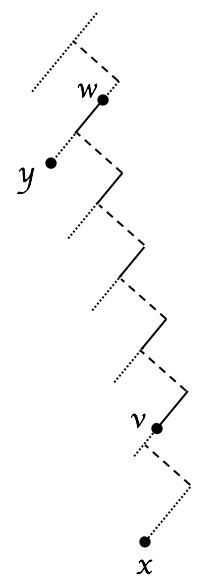
\includegraphics[scale=0.5]{rmq}
        \centering
        \caption[$rmqTree$ query]{Demonstration of an $rmqTree[v, w]$ query. The diagonal lines from right to left are centroid paths of the tree. The parts in bold lie on the path between $v$ and $w$, while those that are dotted do not. Dashed lines connect the root of a centroid path to its parent. $y$ is the leaf at the bottom of the centroid path to which $w$ belongs. $x$ is some leaf in the subtree rooted at $v$.}
        \label{fig:rmq}
    \end{figure}

    \begin{lemma}
        \label{lem:rmqdatastructure}
        Given a tree $T$ and $\weight(u)$ for each $u \in V(T)$, the $rmqTree$ data structure can be built in $O(n\,log\,n)$ time.
    \end{lemma}
        \begin{proof}
            The decomposition step, along with computation of depths for nodes and for centroid paths can be done in $O(n)$ time. Storing the centroid paths in linear RMQ structures takes $O(n)$ time, by Lemma~\ref{lem:linearrmq} and since the total size of the centroid paths is $O(n)$. By the standard argument of centroid-path decomposition, it can be seen that for each leaf $x$, the number of centroid subpaths on the path from the leaf to the root of $T$ is $O(log\,n)$. Hence it takes $O(log\,n)$ time to build the linear RMQ structure for these subpaths. Since there are $n$ leaves, the total time taken to construct the linear RMQ structures for all leaves is $O(n\,log\,n)$.
        \end{proof}

    \medskip
    \begin{lemma}
        \label{lem:rmqquery}
        Given a tree $T$, an $lca$ data structure on $T$, the $rmqTree$ data structure on $T$, and nodes $v, w \in V(T)$ such that $w$ is an ancestor of $v$, the query $rmqTree^T[v, w]$ can be answered in constant time.
    \end{lemma}
        \begin{proof}
            We use the complete centroid path decomposition done when producing the $rmqTree$ data structure. The path from $v$ to $w$ is partitioned into a concatenation of subpaths of these centroid paths, denoted by $Q_1, Q_2, \ldots, Q_g$. This is illustrated in Figure~\ref{fig:rmq}. The diagonal lines from right to left are some of the centroid paths the tree has been decomposed into. The dashed edges indicate that the child is not the heaviest child of its parent, such that the child is the root of a new centroid path. The bold lines are the subpaths of centroid paths that lie on the path from $v$ to $w$. $Q_1$ is the bold centroid subpath starting from $v$ and continuing upwards till the root of that path. Similarly, $Q_g$ is the bold centroid subpath starting at $w$ and continuing downwards until the path splits from that centroid path. $Q_2$ to $Q_{g - 1}$ are the bold centroid subpaths between $Q_1$ and $Q_g$. The significance of the leaves $x$ and $y$ is explained below.

            Take any $x \in \leafset(v)$. Then $Q_2, \ldots, Q_{g - 1}$ are contained fully in the centroid subpaths on the path from $x$ to the root of $T$. $Q_1$ must be a subpath that starts at $v$ in some centroid path $\in \mathcal{P}(T)$ and ends at the root of that centroid path. $Q_g$ is a subpath that starts at some node in some centroid path $\in \mathcal{P}(T)$ and ends at $w$, within the same path. We address each of these three divisions separately.

            To find the maximum weight within $Q_1$, we obtain the depth of $v$ within $Q_1$ by subtracting the depth of the root of $Q_1$ from the depth of $v$. Then the maximum weight can be retrieved by querying the linear RMQ structure for this centroid path, from the root to $v$ (recall that the depths and linear RMQ structures were obtained while constructing the $rmqTree$ data structure). Querying the linear RMQ structure costs constant time, as set out in Lemma~\ref{lem:linearrmq}.

            To find the maximum weight for the subpaths $Q_2, \ldots, Q_{g - 1}$, we obtain the indices of $Q_2$ and $Q_{g-1}$ in $W_x$ as $depth^{T}(Q_1) + 1$ and $depth^{T}(Q_g) - 1$ respectively. The maximum weight can then be found by querying $W_x$.

            Finally, we need to find the maximum weight within $Q_g$. Observe that the key here is finding which node is at the end of $Q_g$. Let $P_i \in \mathcal{P}(T)$ be the centroid path of which $Q_g$ is a subpath. Then the previous question is equivalent to finding which node in $P_i$ has $v$ in one of its side trees. Let $y$ be the leaf at the bottom of $P_i$. Then the desired node is simply $lca(y, v)$, querying for which takes $O(1)$ time as given by Lemma~\ref{lem:lca}. The maximum weight within $Q_g$ can now be easily found in constant time by querying the linear RMQ structure for $P_i$, from $w$ to $lca(y, v)$.

            As of these three values can be obtained in constant time, the query as a whole takes $O(1)$ time.
        \end{proof}

    \subsection{Querying maximum weight among nodes on an open path of a weighted tree}
    \label{subsec:cfd}

    Given a weighted tree $T$, previous subsection provides a data structure to compute $rmqTree^T[v, w]$ where $w$ is an ancestor of $v$ in $T$. Here, we extend the data structure to compute $rmqTree^T(v, w) = max_{u \in path^T(v, w)} \weight(u)$. Note that the parentheses indicate exclusion of the two endpoints $v$ and $w$. Precisely, let $childD(v, w)$ be the child of $w$ that is an ancestor of $v$; then, $rmqTree^T(v, w) = rmqTree^T[parent(v), childD(v,w)]$.
    Similarly, we define $rmqTree^T[v, w) = rmqTree^T[v, childD(v,w)]$ and $rmq^T(v, w] = rmqTree^T[parent(v), w)$.

    Note that $parent(v)$ can be answered in constant time. If there exists a data structure that enables $childD(v,w)$ to be computed in $O(1)$ time, we have a data structure that answers the $rmqTree^T(v, w)$,  $rmqTree^T[v, w)$ and $rmq^T(v, w]$. Below, we describe such a data structure.

%    Given a tree $T$ and nodes $v, w \in V(T)$ such that $w$ is a proper ancestor of $v$, define $childD(v, w)$ as the child of $w$ that is an ancestor of $v$. We construct a data structure that allows us to answer this query in constant time, given $O(n\,log\,n)$ preprocessing time, where $n = |V(T)|$.

    Reorder $T$ such that the heaviest child of each node is its leftmost child. Then the leaves of $T$ are indexed in left to right order, such that every leaf $x \in \leafset^T$ is assigned a value $index(x)$. Then for every node $u \in V(T)$, the indices of the leaves in $T[u]$ form a consecutive range. For each internal node $u \in V(T)$, define its side children to be the set $children(u) - \{\text{heaviest child of }u\}$ and its side trees to be the subtrees of $T$ rooted at its side children. Let $x$ and $y$ be the leaves in the side trees of $u$ with the smallest and largest indices respectively. We now build the array $cFL_u[0\, \ldots\, index(y) - index(x)]$ which maps each leaf $z$ in the side trees of $u$ to the child of $u$ that is an ancestor of $z$. Thus, for every leaf $z$ in $T[v]$ for some $v \in$ side children of $u$, let $cFL_u[index(z) - index(x)] = v$.
    \newline

    \begin{lemma}
        \label{lem:cfddatastructure}
        Given a tree $T$ where $n = |V(T)|$, the $cFL$ data structure defined above can be constructed in $O(n\,log\,n)$ time.
    \end{lemma}
        \begin{proof}
            Rearranging $T$ and indexing the leaves can be done in two $O(n)$ passes. By the standard argument of centroid-path decomposition, we argue that any leaf is in the side trees of $O(log\,n)$ nodes, hence the total size of the $cFL$ arrays is $O(n\,log\,n)$. It is easy to see that these arrays can thus be constructed in $O(n\,log\,n)$ time.
        \end{proof}

    \medskip
    \begin{lemma}
        \label{lem:cfdquery}
        Given a tree $T$, an $lca$ data structure on $T$, the $cFL$ data structure on $T$ and nodes $v, w \in V(T)$, the query $childD(v, w)$ can be answered in constant time.
    \end{lemma}
        \begin{proof}
            The query is divided into two parts. First, we check if $v$ is a descendant of the heaviest child of $w$. If so, we are done. If not, we need to determine which child of $w$ is an ancestor of $v$.

            To answer the first part, we can see that, given nodes $r, s \in V(T)$, $s$ is an ancestor of $r$ iff $lca(r, s) = s$. Thus we can check if $v$ is a descendant of the heaviest child of $w$ in $O(1)$ time since by Lemma~\ref{lem:lca}, the $lca$ data structure allows queries in constant time.

            For the second part, we simply retrieve the entry corresponding to any leaf in $\leafset(v)$ from $cFL_w$, again easily done in constant time.
        \end{proof}

Putting together Lemmas~\ref{lem:rmqquery} and \ref{lem:cfdquery}, we have the following result.
    \begin{theorem}
        \label{theorem:rmqtreequery}
        Given a weighted tree $T$, the $rmqTree$ data structure on $T$ can be built in $O(n\,log\,n)$ time, allowing answering the queries $rmqTree(v, w)$, $rmqTree[v, w)$, $rmqTree(v, w]$, $rmqTree[v, w]$ in constant time for any nodes $v, w \in V(T)$ such that $w$ is an ancestor of $v$.
    \end{theorem}
%        \begin{proof}
%            Observe that $rmqTree^{T}(v, w) = rmqTree^{T}[parent(v), childD(v, w)]$. Thus it is clear that using the $childD$ structure and an RMQ structure, we can answer these queries in constant time. Building both these structures costs $O(n\,log\,n)$ time.
%        \end{proof}



    \section{Implementation}
    \label{sec:implementation}

    As noted in Section~\ref{subsec:previouswork}, there are two existing implementations that compute FDCTs - TNT \cite{goloboff2008tnt} and the FACT package \cite{jansson2016improved}. However, the results in \cite{jansson2018algorithms} demonstrated that their implementation outperforms TNT under all conditions, so we only make a comparison with the FACT package. Our implementation of the algorithm \texttt{Frequency\_Difference} reuses their code, with certain key optimisations, as laid out above. The code is written in C++ and utilises some libraries from the Boost package \cite{BoostLibrary}. The source can be found at \url{https://github.com/varung97/FACT2}. Note that there are some differences between the implementation and the algorithm described above, made for reasons of optimisation and readability. These differences are described in Section~\ref{subsec:implementationdetails}.

    The resulting implementation was compared with that from the FACT package by running them both on trees generated with various values of $k$ and $n$. This setup is described in Section~\ref{subsec:setup} and the results are presented in Section~\ref{subsec:results}.

    \subsection{Implementation Details}
    \label{subsec:implementationdetails}

    The differences between the described algorithm and our implementation are:

    \begin{enumerate}
        \item While the algorithm is fully deterministic, the implementation is not; we use hash sets instead of linked lists to store nodes in the minimum cover for ease.

        \item The algorithm \texttt{Find\_Coverer} is implemented iteratively instead of recursively for efficiency. Further, this procedure and the procedure \texttt{Update\_Incompatible} were moved inside the main body of the algorithm rather than separating them out into functions, again because this is faster.

        \item Rather than constructing the trees $\TB||\leafset^{\tau}$ and then inserting the nodes on certain paths into the Brodal queue, we simply obtain the maximum weight of nodes on the paths using $rmqTree$ queries and insert this maximum weight into the queue.
    \end{enumerate}

    \subsection{Experimental Setup}
    \label{subsec:setup}

    We generated input trees according to two different scenarios, exactly as in \cite{jansson2018algorithms}. The first scenario, ``Scenario 1'', is the situation where trees share a large percentage of clusters, which is largely realistic. On the other hand, the second scenario, ``Scenario 2'', generates completely independent trees, which represents the other end of the spectrum. In particular, the process for generating $k$ trees with leaf labels $\{1, 2, \dots, n\}$ under the two scenarios is:

    \begin{itemize}
        \item \textit{Scenario 1:} We generate a binary tree, with the given leaf labels, under the uniform model \cite{mckenzie2000distributions}. Then for each non-root internal node $u$ in this tree, we perform a $delete$ operation on $u$ with probability $0.2$. Then we make $k$ copies of this tree, and for each copy, we randomly select a non-root node $u$ and an internal node $v$ $n / 20$ times, remove the subtree rooted at $u$ and attach it to $v$.

        \item \textit {Scenario 2:} We generate $k$ binary trees, with the given leaf labels, each under the uniform model \cite{mckenzie2000distributions}. Then for each non-root internal node $u$ in each tree, we $delete$ $u$ with probability $0.2$.
    \end{itemize}

    Since we wished to see the effect of both $k$ and $n$ on these algorithms, we ran two experiments, one with $n$ fixed and one with $k$ fixed. Further, we measured the time taken by the weighting step and the remainder of the algorithm separately. Note that we use the running time of the second half of \texttt{Frequency\_Difference} as a stand-in for running time of \texttt{Filter\_Clusters} as it is hard to measure the latter independently, and since the implementations are identical except for \texttt{Filter\_Clusters}. For each value of $k$ and $n$, we generated 5 input examples and averaged the running time over these.

    We ran the experiments on a MacBook Pro laptop running macOS Sierra 10.12.6, equipped with 16GB RAM and a 2.2 GHz Intel Core i7 processor. The C++ compiler used was clang-802.0.42 and the version of the Boost libraries was 1.65.1. The time taken was measured using the inbuilt \texttt{clock()} function in C++.

    \subsection{Experimental Results}
    \label{subsec:results}

    \begin{table}[!ht]
        \captionsetup{font=footnotesize,justification=justified,margin=0cm}
        \small
        \begin{minipage}{0.48\textwidth}
            \centering
            \caption{Weighting time with $n = 1000$, varying $k$}
            \label{tab:weightk1}
            \begin{tabular}{c||ccccc}
                $k$ & $kn\,log\,n$ & $kn^2$ & $k^2n$\\
                \hline\hline
                50 & 0.34 & 0.04 & 0.04\\
                100 & 0.66 & 0.09 & 0.12\\
                200 & 1.32 & 0.17 & 0.46\\
                500 & 3.51 & 0.47 & 2.82\\
                1000 & 7.32 & 1.03 & 11.25\\
                2000 & 15.07 & 2.27 & 45.13\\
                3000 & 23.58 & 3.66 & 100.06\\
                4000 & 31.48 & 4.87 & 174.49\\
            \end{tabular}
            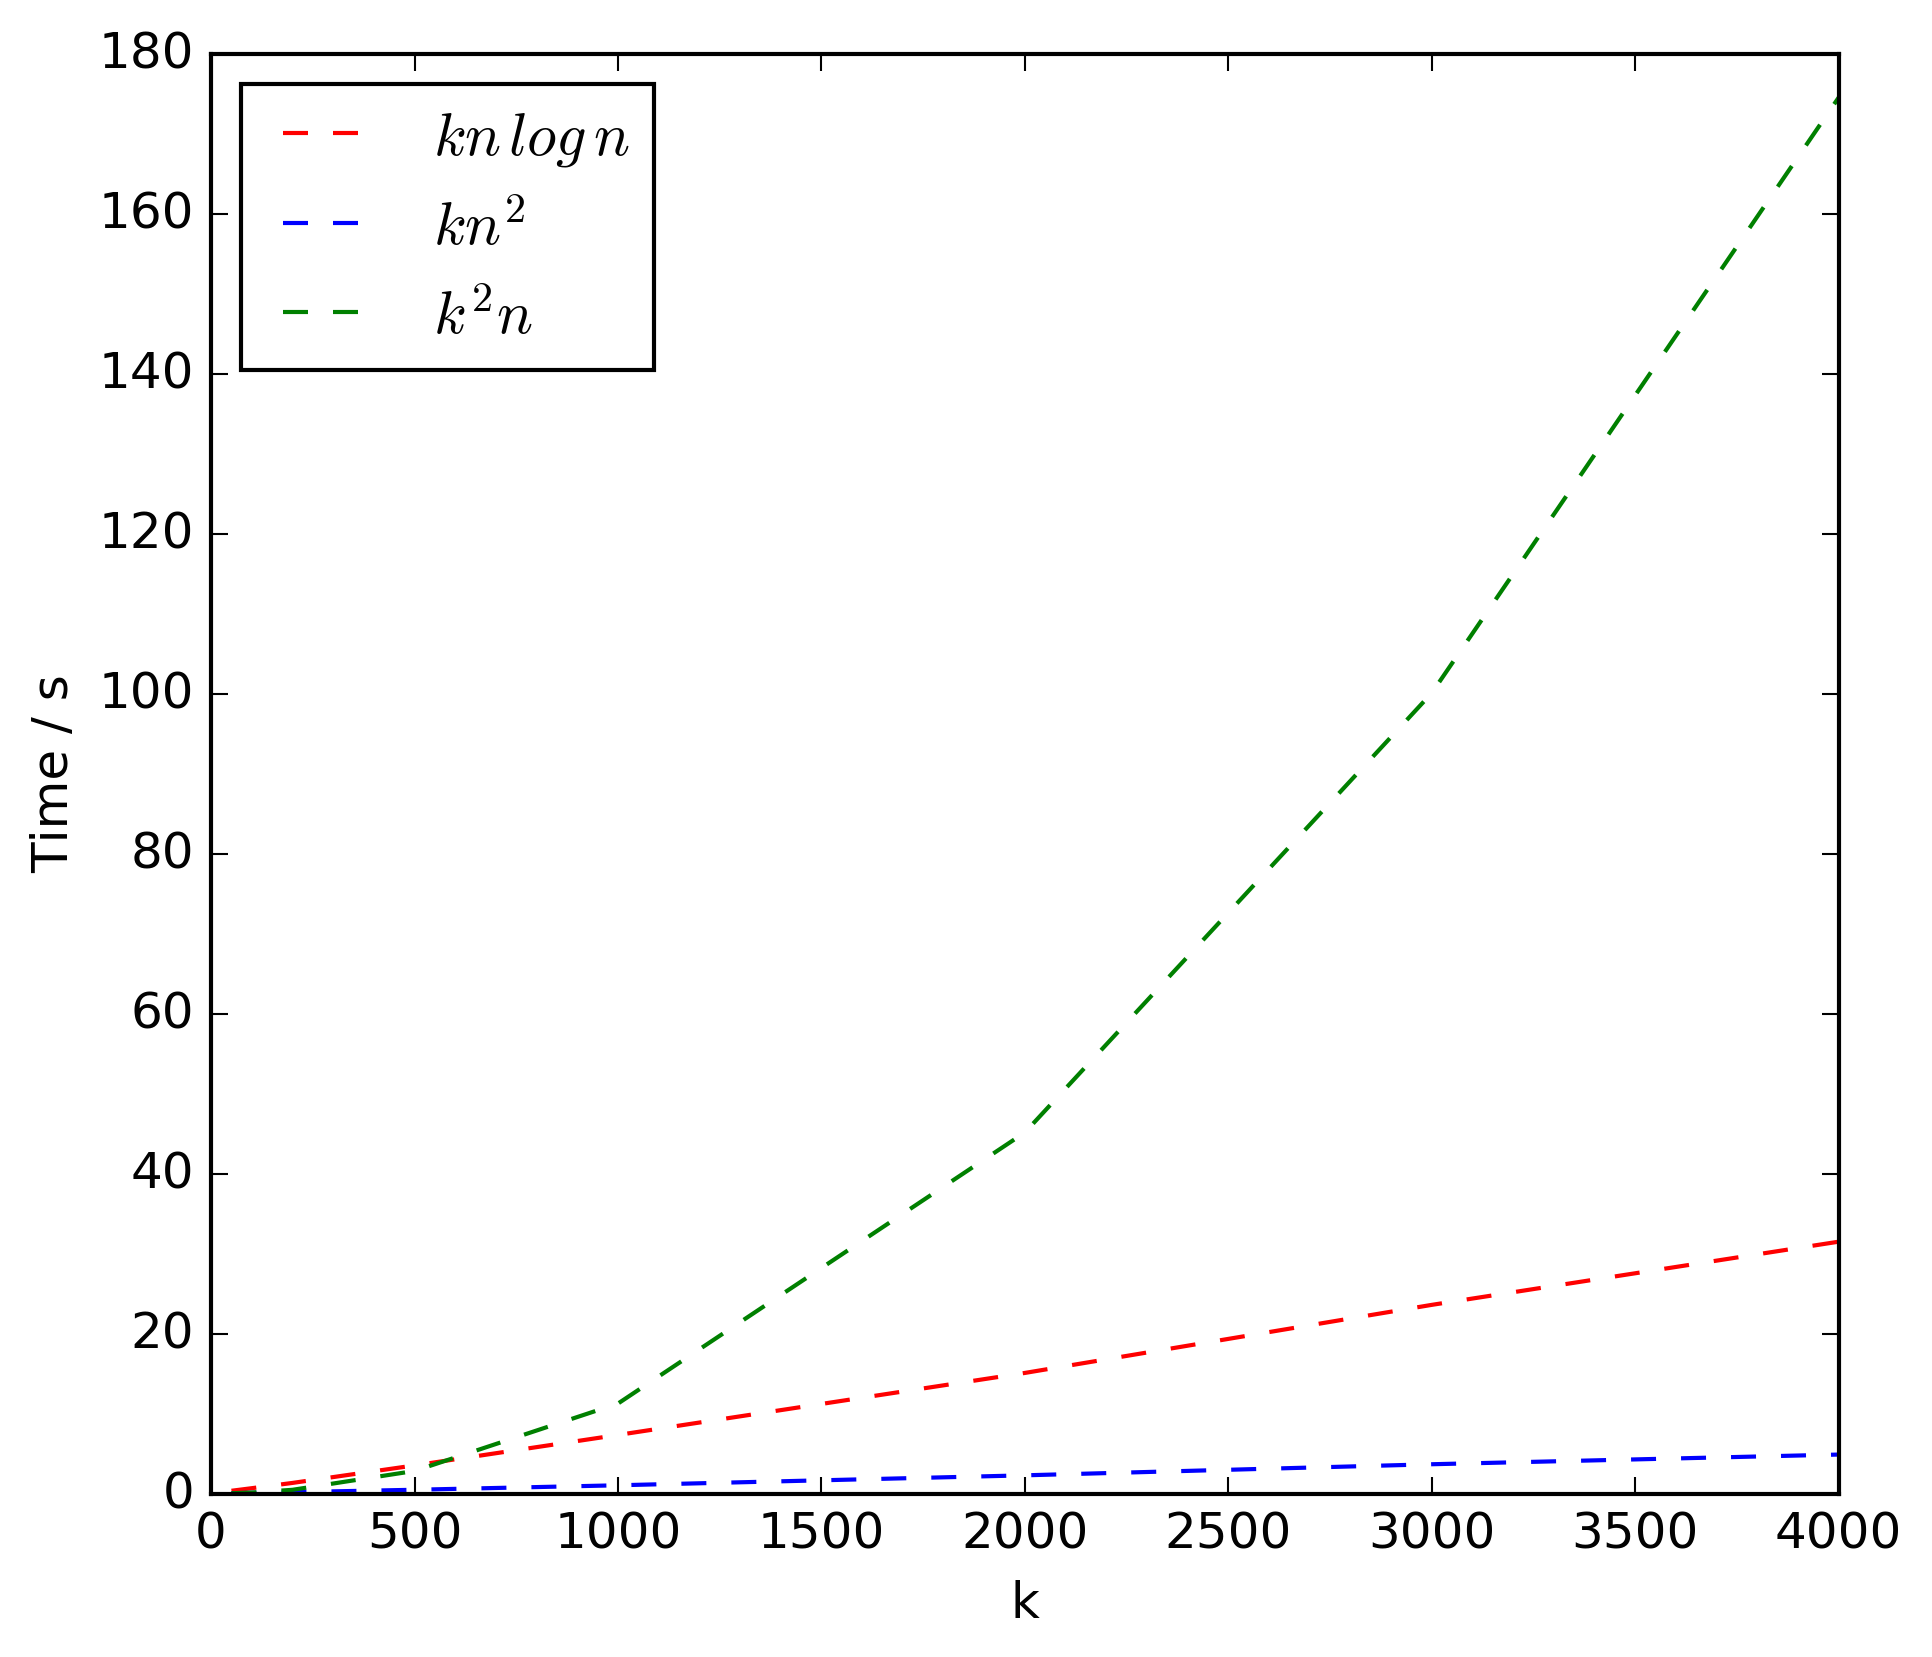
\includegraphics[scale=0.4]{varyingk1_weighting}
            \vspace{0.5cm}
        \end{minipage}\hfill
        \begin{minipage}{0.48\textwidth}
            \centering
            \caption{\texttt{Filter\_Clusters} time with $n = 1000$, varying $k$}
            \label{tab:filterk1}
            \begin{tabular}{c||ccccc}
                $k$ & $n\,log\,n$ & $n\,log^2n$\\
                \hline\hline
                50 & 1.13 & 1.04\\
                100 & 2.31 & 2.52\\
                200 & 4.65 & 5.00\\
                500 & 11.89 & 13.90\\
                1000 & 24.84 & 27.39\\
                2000 & 52.71 & 62.18\\
                3000 & 81.01 & 84.99\\
                4000 & 108.53 & 116.16\\
            \end{tabular}
            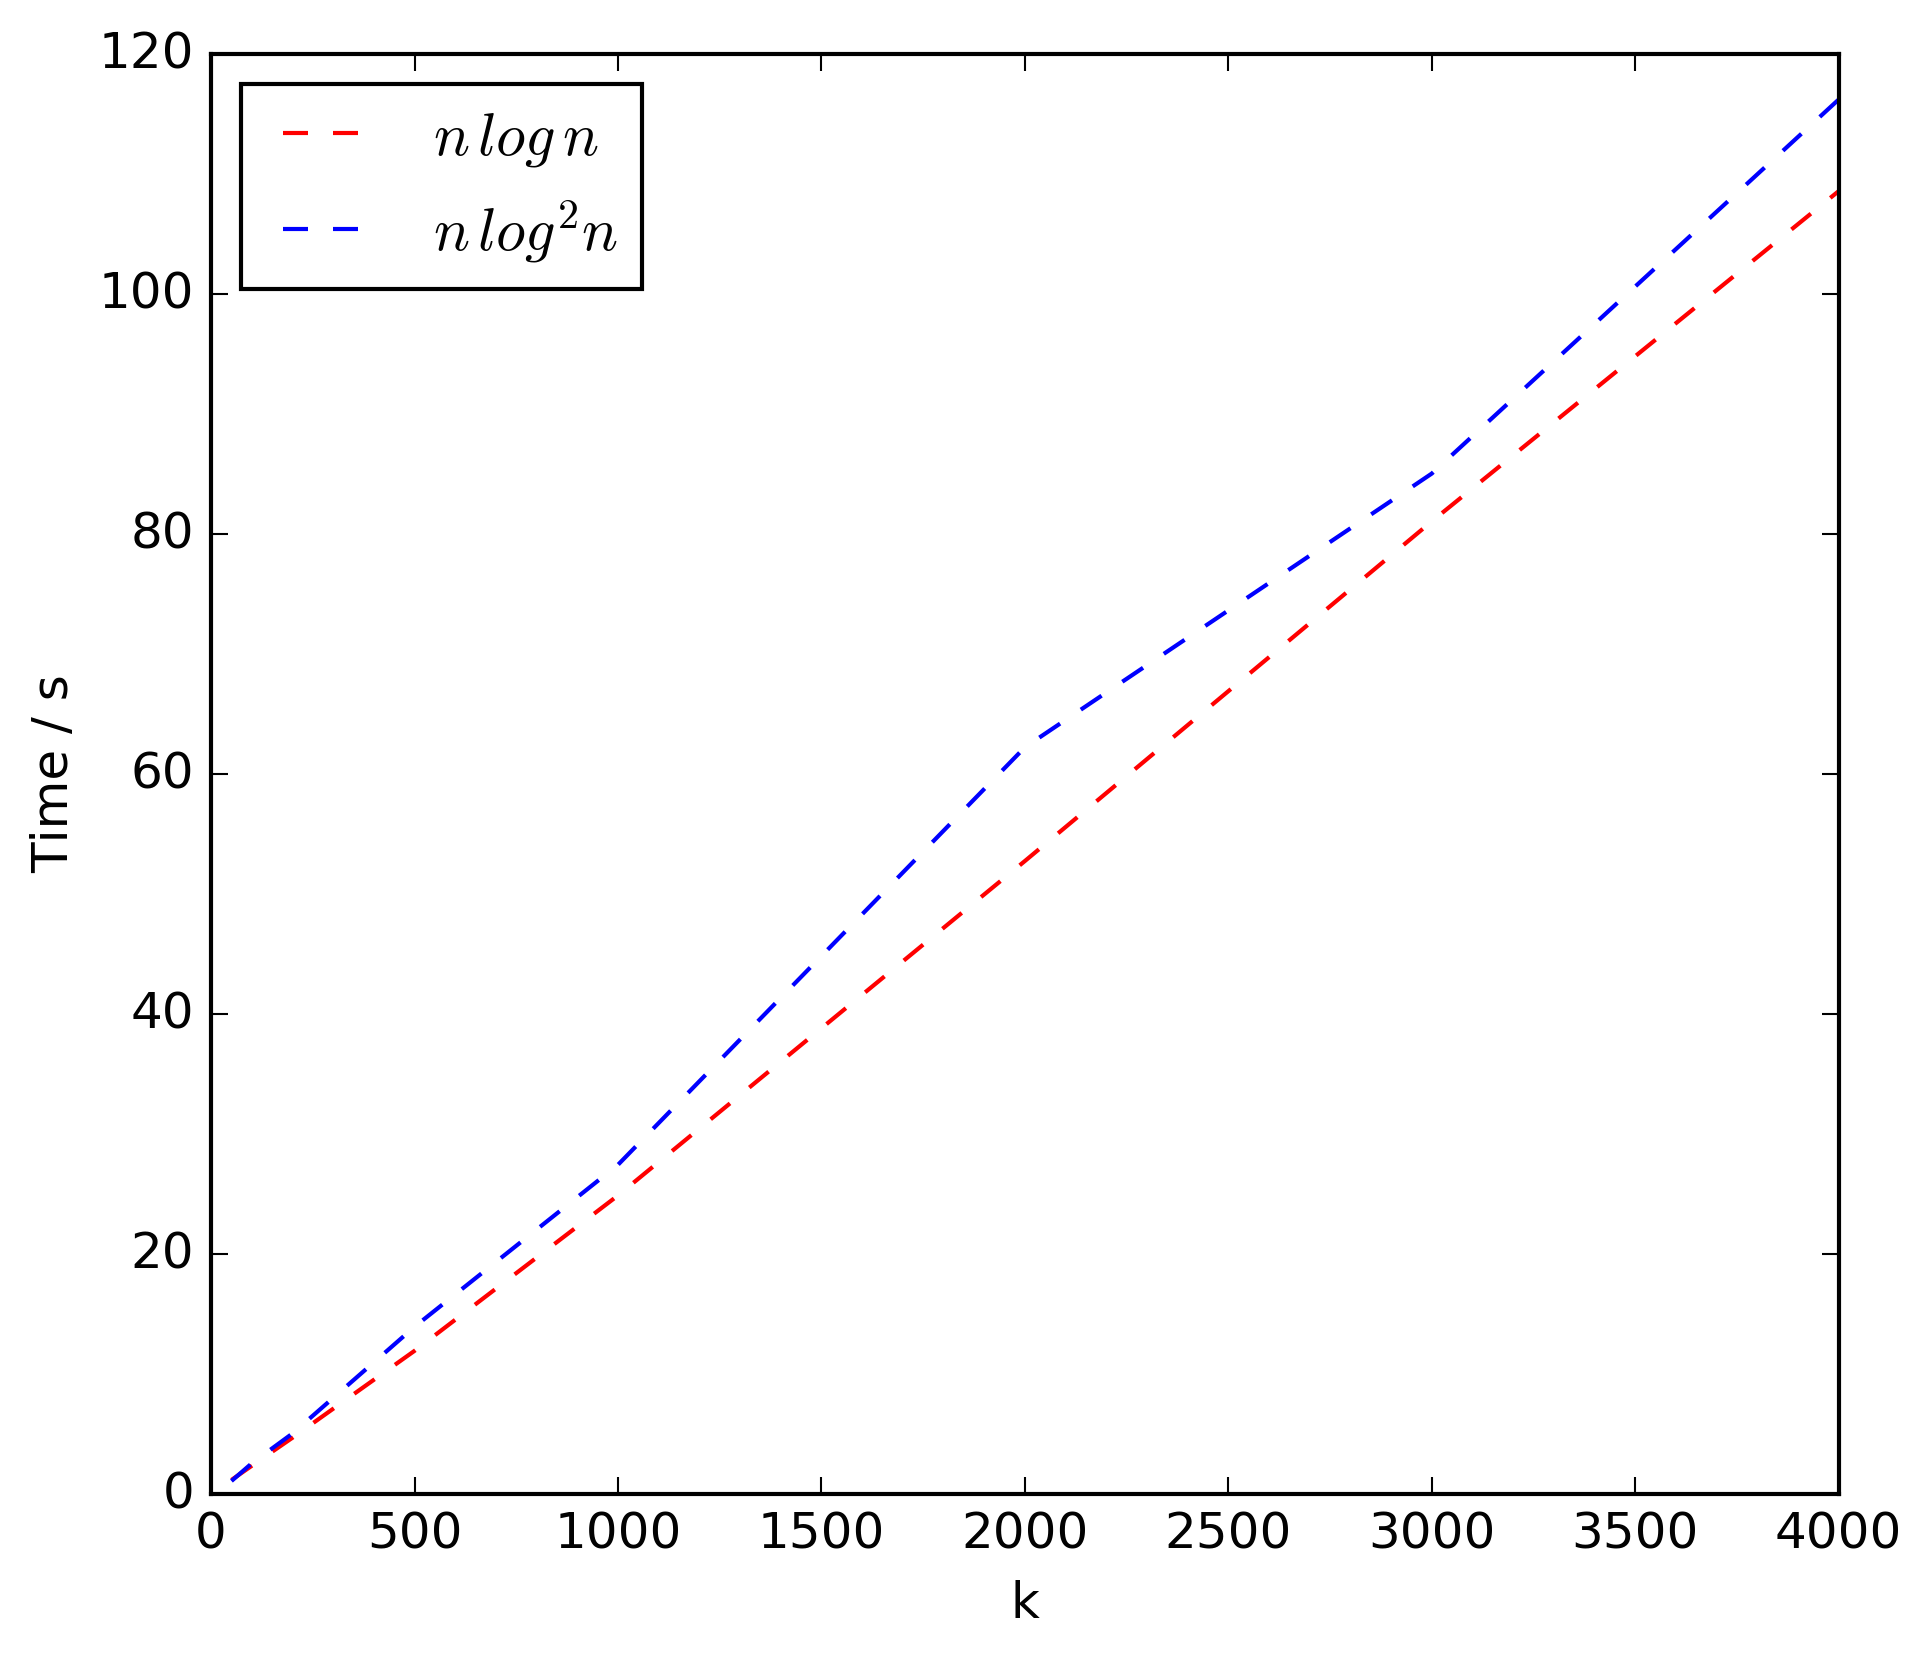
\includegraphics[scale=0.4]{varyingk1_filter}
            \vspace{0.5cm}
        \end{minipage}
        \begin{minipage}{0.48\textwidth}
            \centering
            \caption{Weighting time with $k = 100$, varying $n$}
            \label{tab:weightn1}
            \begin{tabular}{c||ccccc}
                $n$ & $kn\,log\,n$ & $kn^2$ & $k^2n$\\
                \hline\hline
                1000 & 0.65 & 0.08 & 0.11\\
                2000 & 1.40 & 0.23 & 0.23\\
                3000 & 2.21 & 0.43 & 0.36\\
                4000 & 3.06 & 0.68 & 0.47\\
                5000 & 3.92 & 1.06 & 0.60\\
                7500 & 6.09 & 2.08 & 0.90\\
                10000 & 8.36 & 3.65 & 1.22\\
                20000 & 19.13 & 12.08 & 2.73\\
                30000 & 30.02 & 35.94 & 4.05\\
            \end{tabular}
            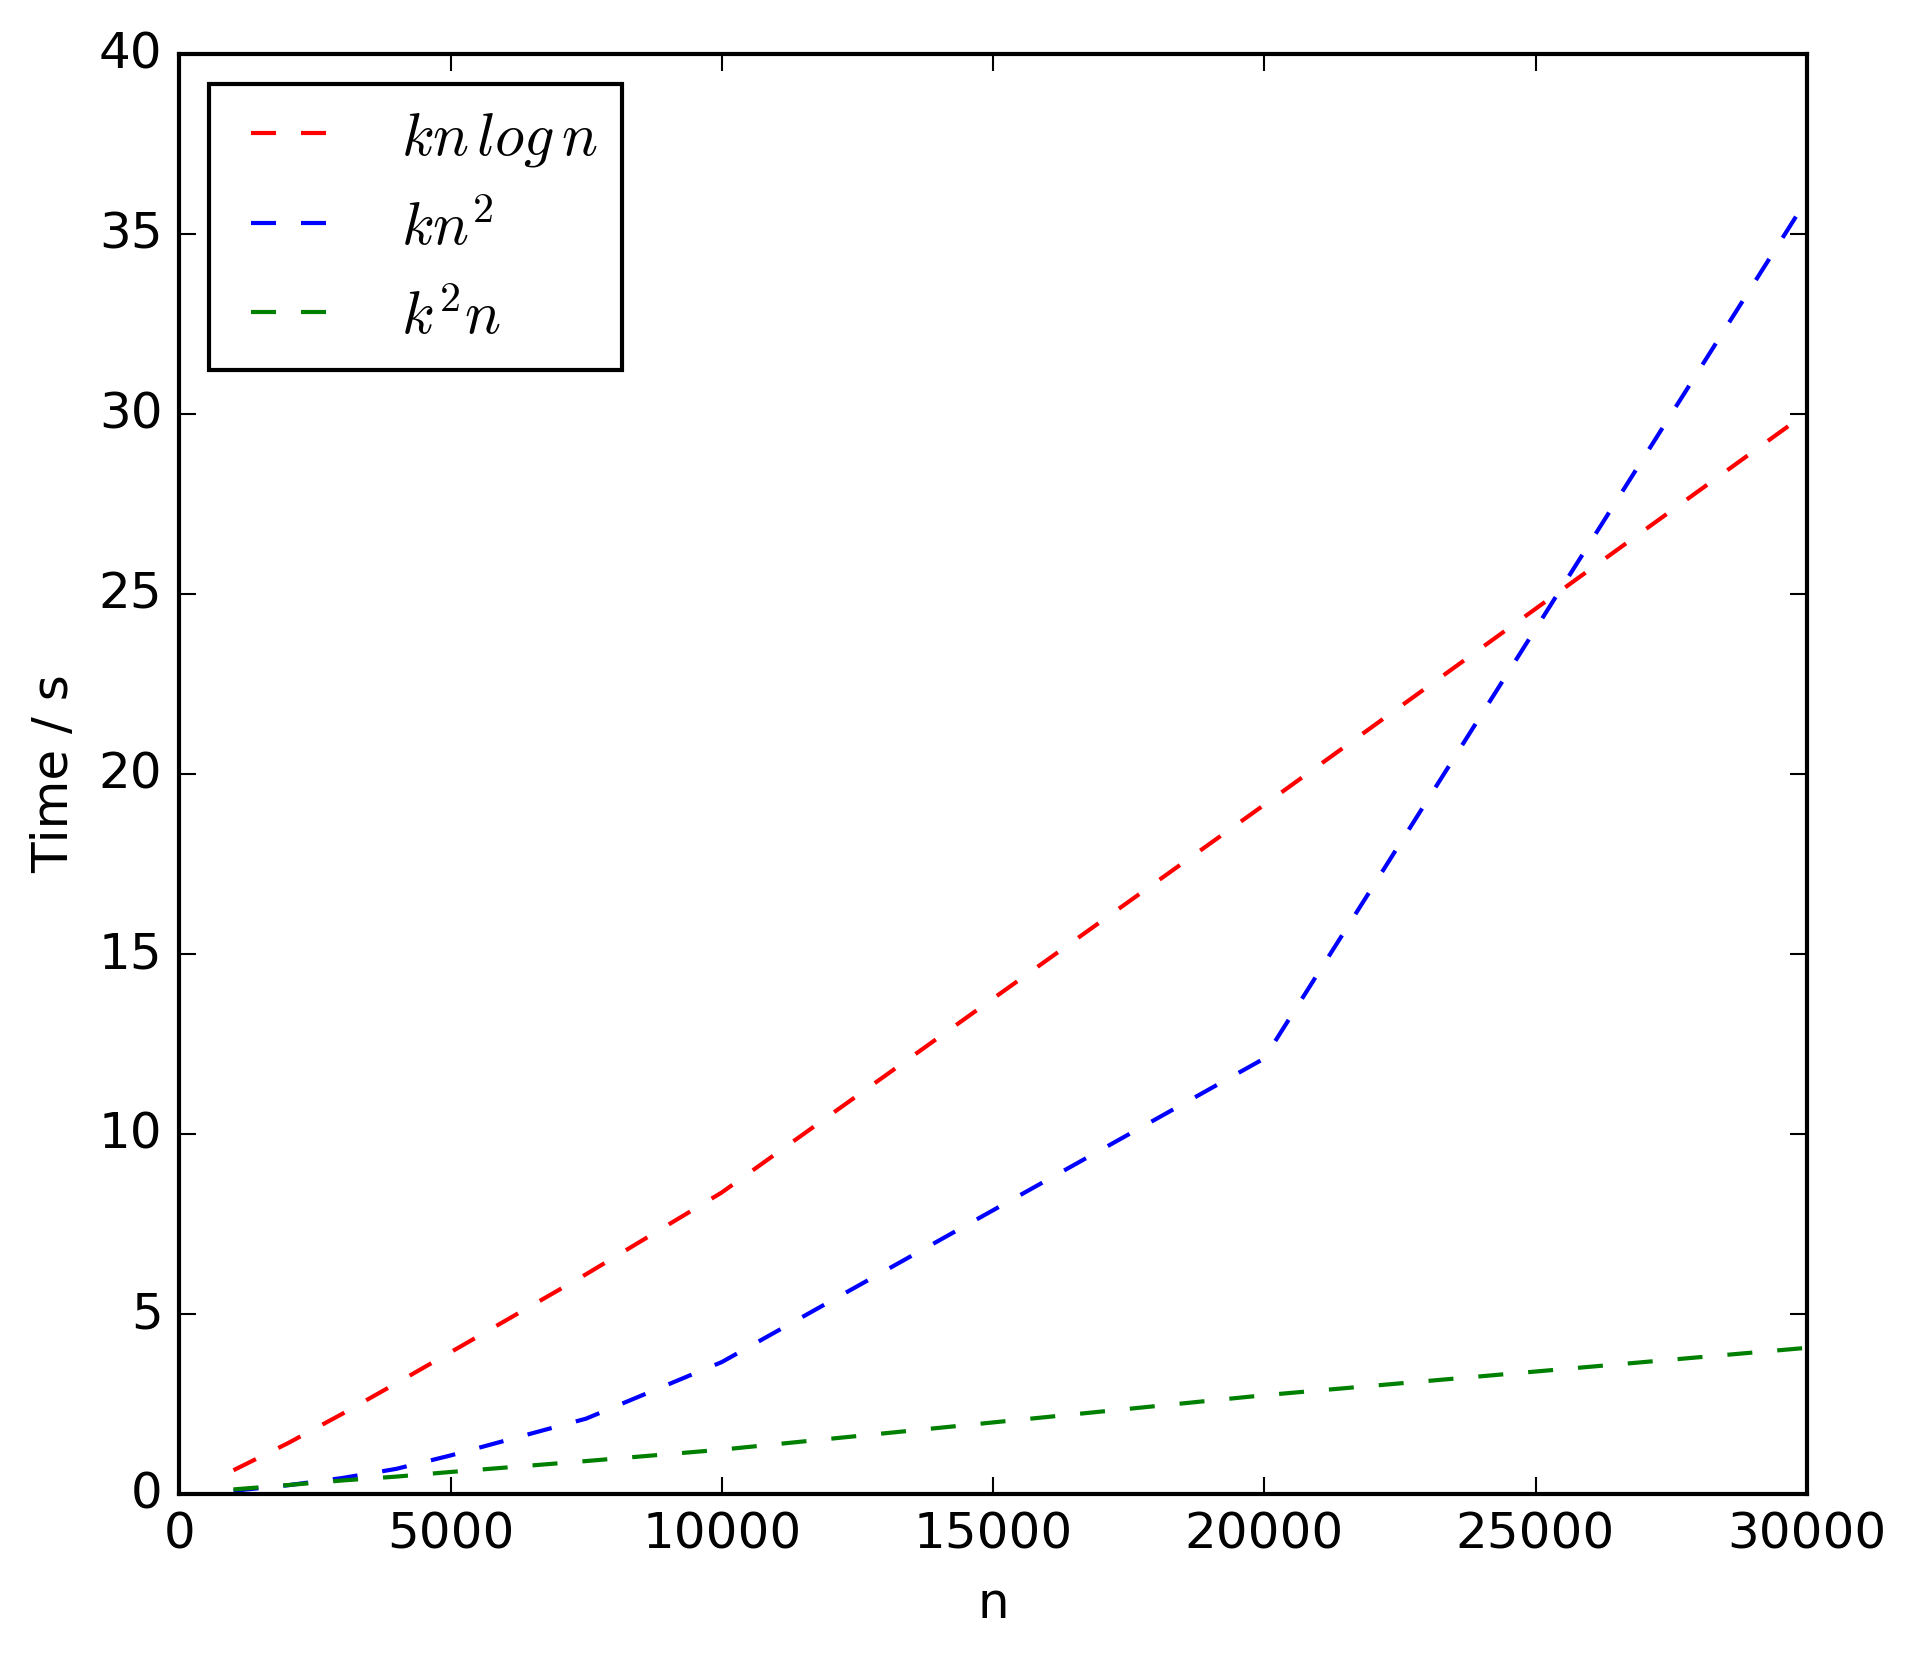
\includegraphics[scale=0.4]{varyingn1_weighting}
        \end{minipage}\hfill
        \begin{minipage}{0.48\textwidth}
            \centering
            \caption{\texttt{Filter\_Clusters} time with $k = 100$, varying $n$}
            \label{tab:filtern1}
            \begin{tabular}{c||ccccc}
                $n$ & $n\,log\,n$ & $n\,log^2n$\\
                \hline\hline
                500 & 1.09 & 0.51\\
                1000 & 2.22 & 2.42\\
                1500 & 3.33 & 10.86\\
                2000 & 4.54 & 17.74\\
                3000 & 7.06 & 31.29\\
                4000 & 9.62 & 49.92\\
                5000 & 12.20 & 69.88\\
                7500 & 18.54 & 129.07\\
                10000 & 25.38 & 211.64\\
            \end{tabular}
            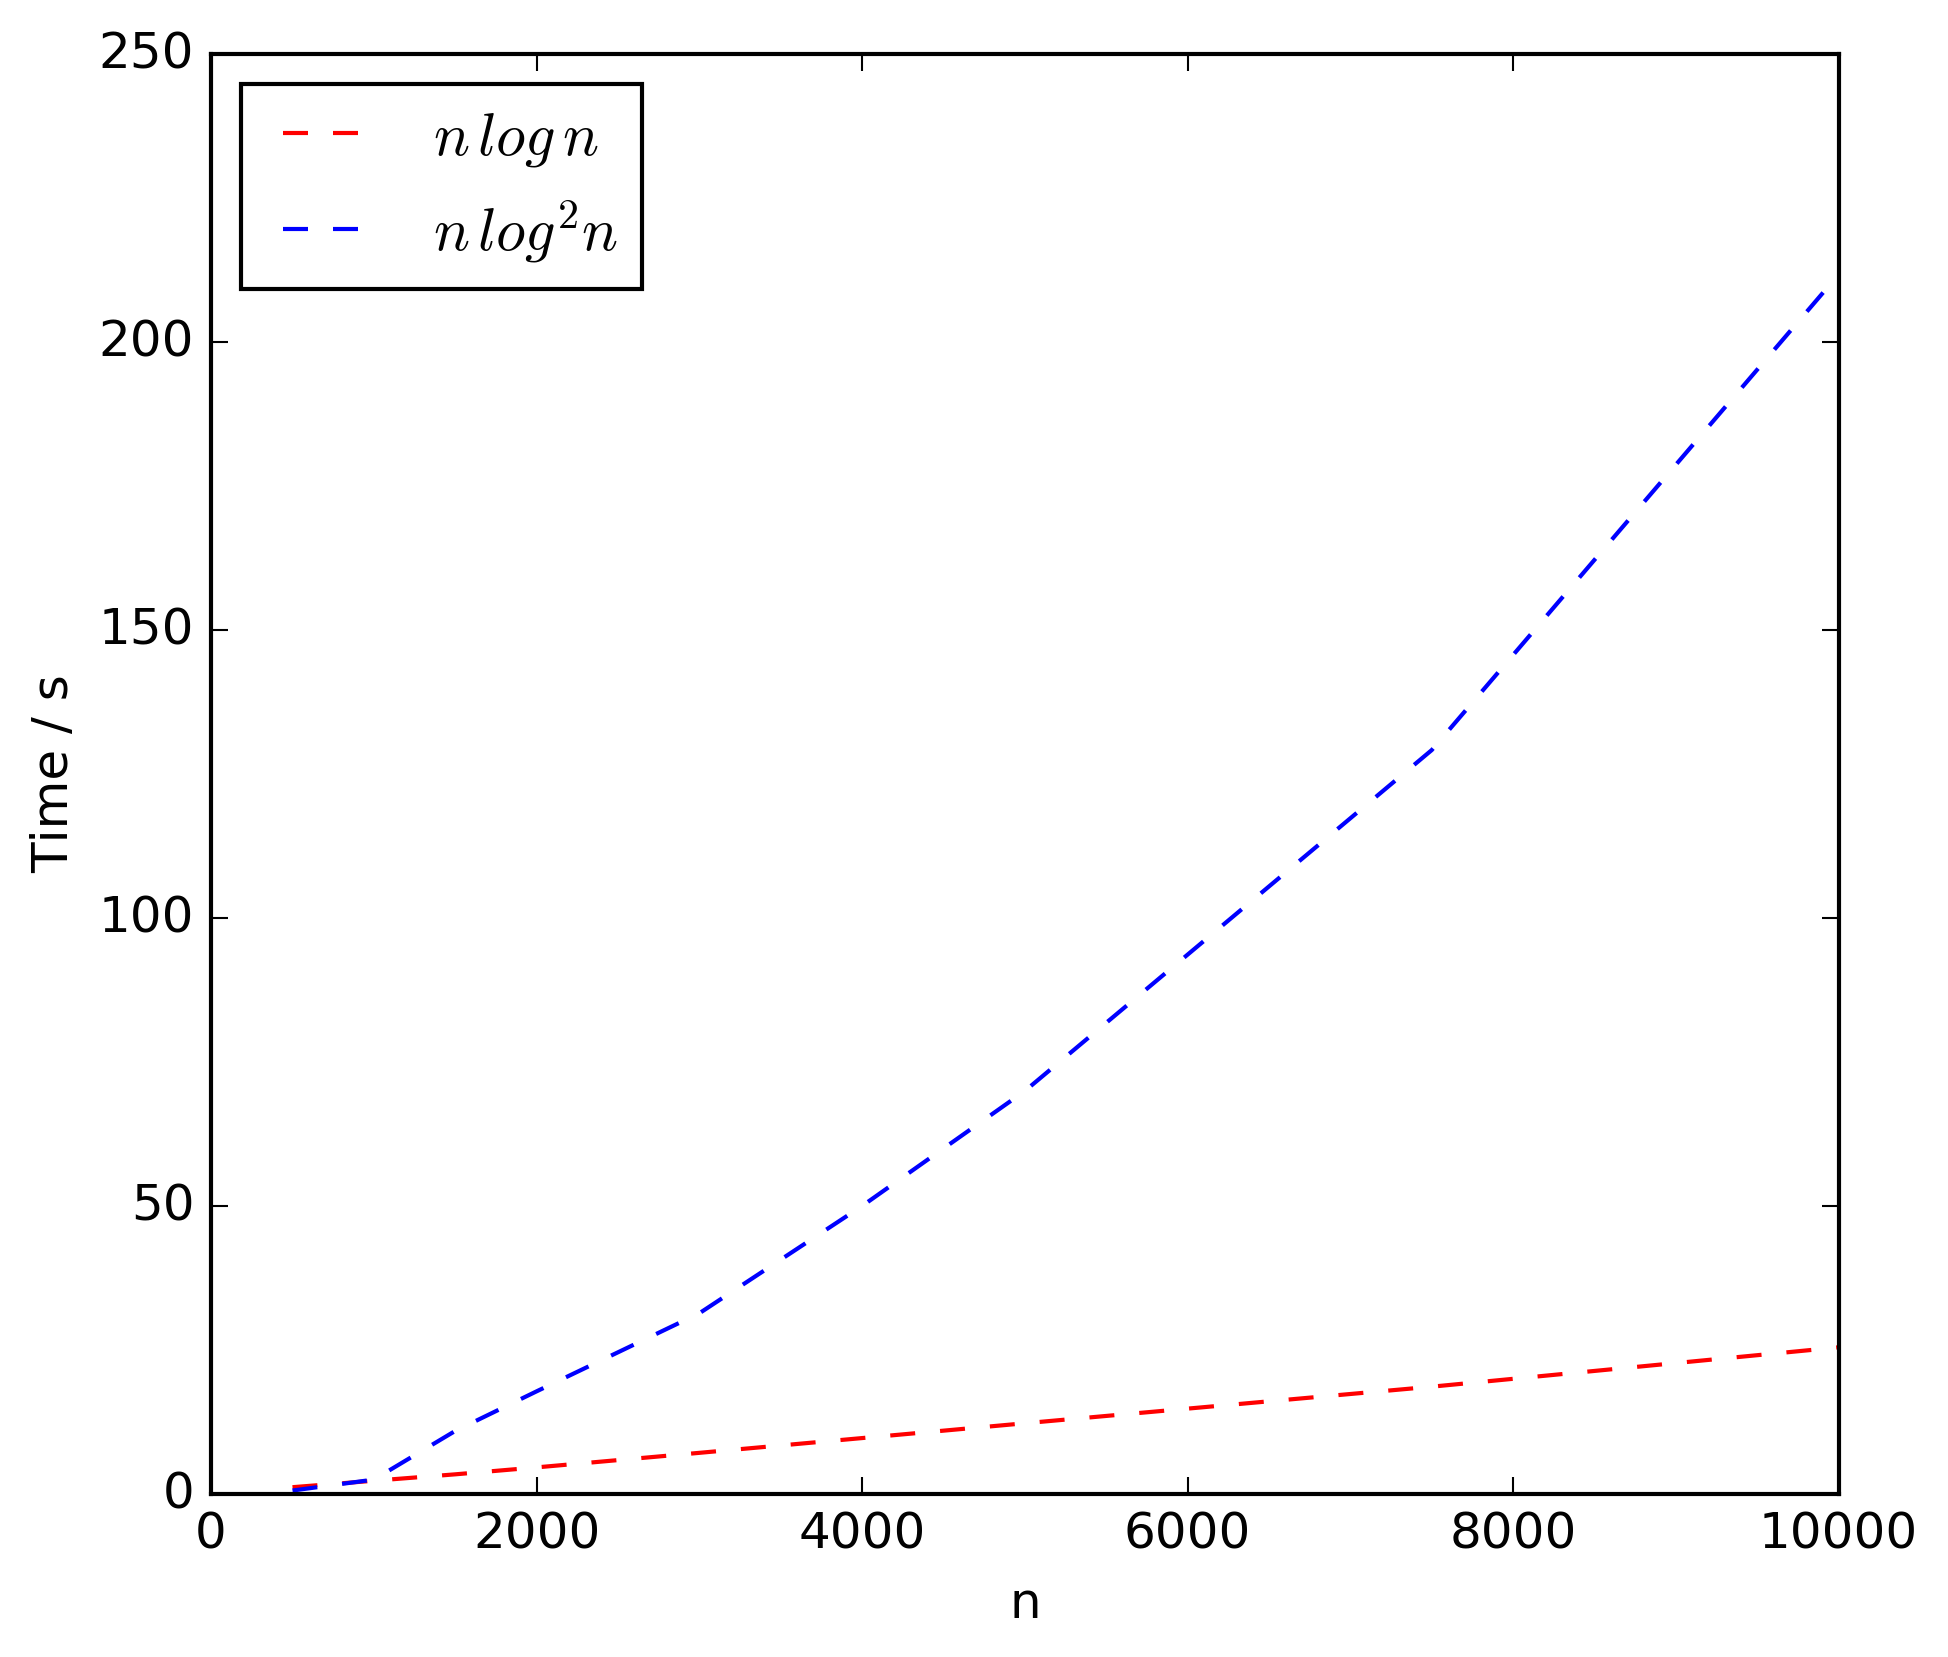
\includegraphics[scale=0.4]{varyingn1_filter}
        \end{minipage}
        \captionof{figure}{Experimental Results for Scenario $1$}
        \label{fig:expresults1}
    \end{table}

    \begin{table}[!ht]
        \captionsetup{font=footnotesize,justification=justified,margin=0cm}
        \small
        \begin{minipage}{0.48\textwidth}
            \centering
            \caption{Weighting time with $n = 1000$, varying $k$}
            \label{tab:weightk2}
            \begin{tabular}{c||ccccc}
                $k$ & $kn\,log\,n$ & $kn^2$ & $k^2n$\\
                \hline\hline
                50 & 0.41 & 0.04 & 0.03\\
                100 & 0.80 & 0.08 & 0.10\\
                200 & 1.57 & 0.18 & 0.37\\
                500 & 4.10 & 0.50 & 2.29\\
                1000 & 8.62 & 1.09 & 8.95\\
                2000 & 17.56 & 2.39 & 35.30\\
                3000 & 27.30 & 3.71 & 79.17\\
                4000 & 37.71 & 5.16 & 140.47\\
            \end{tabular}
            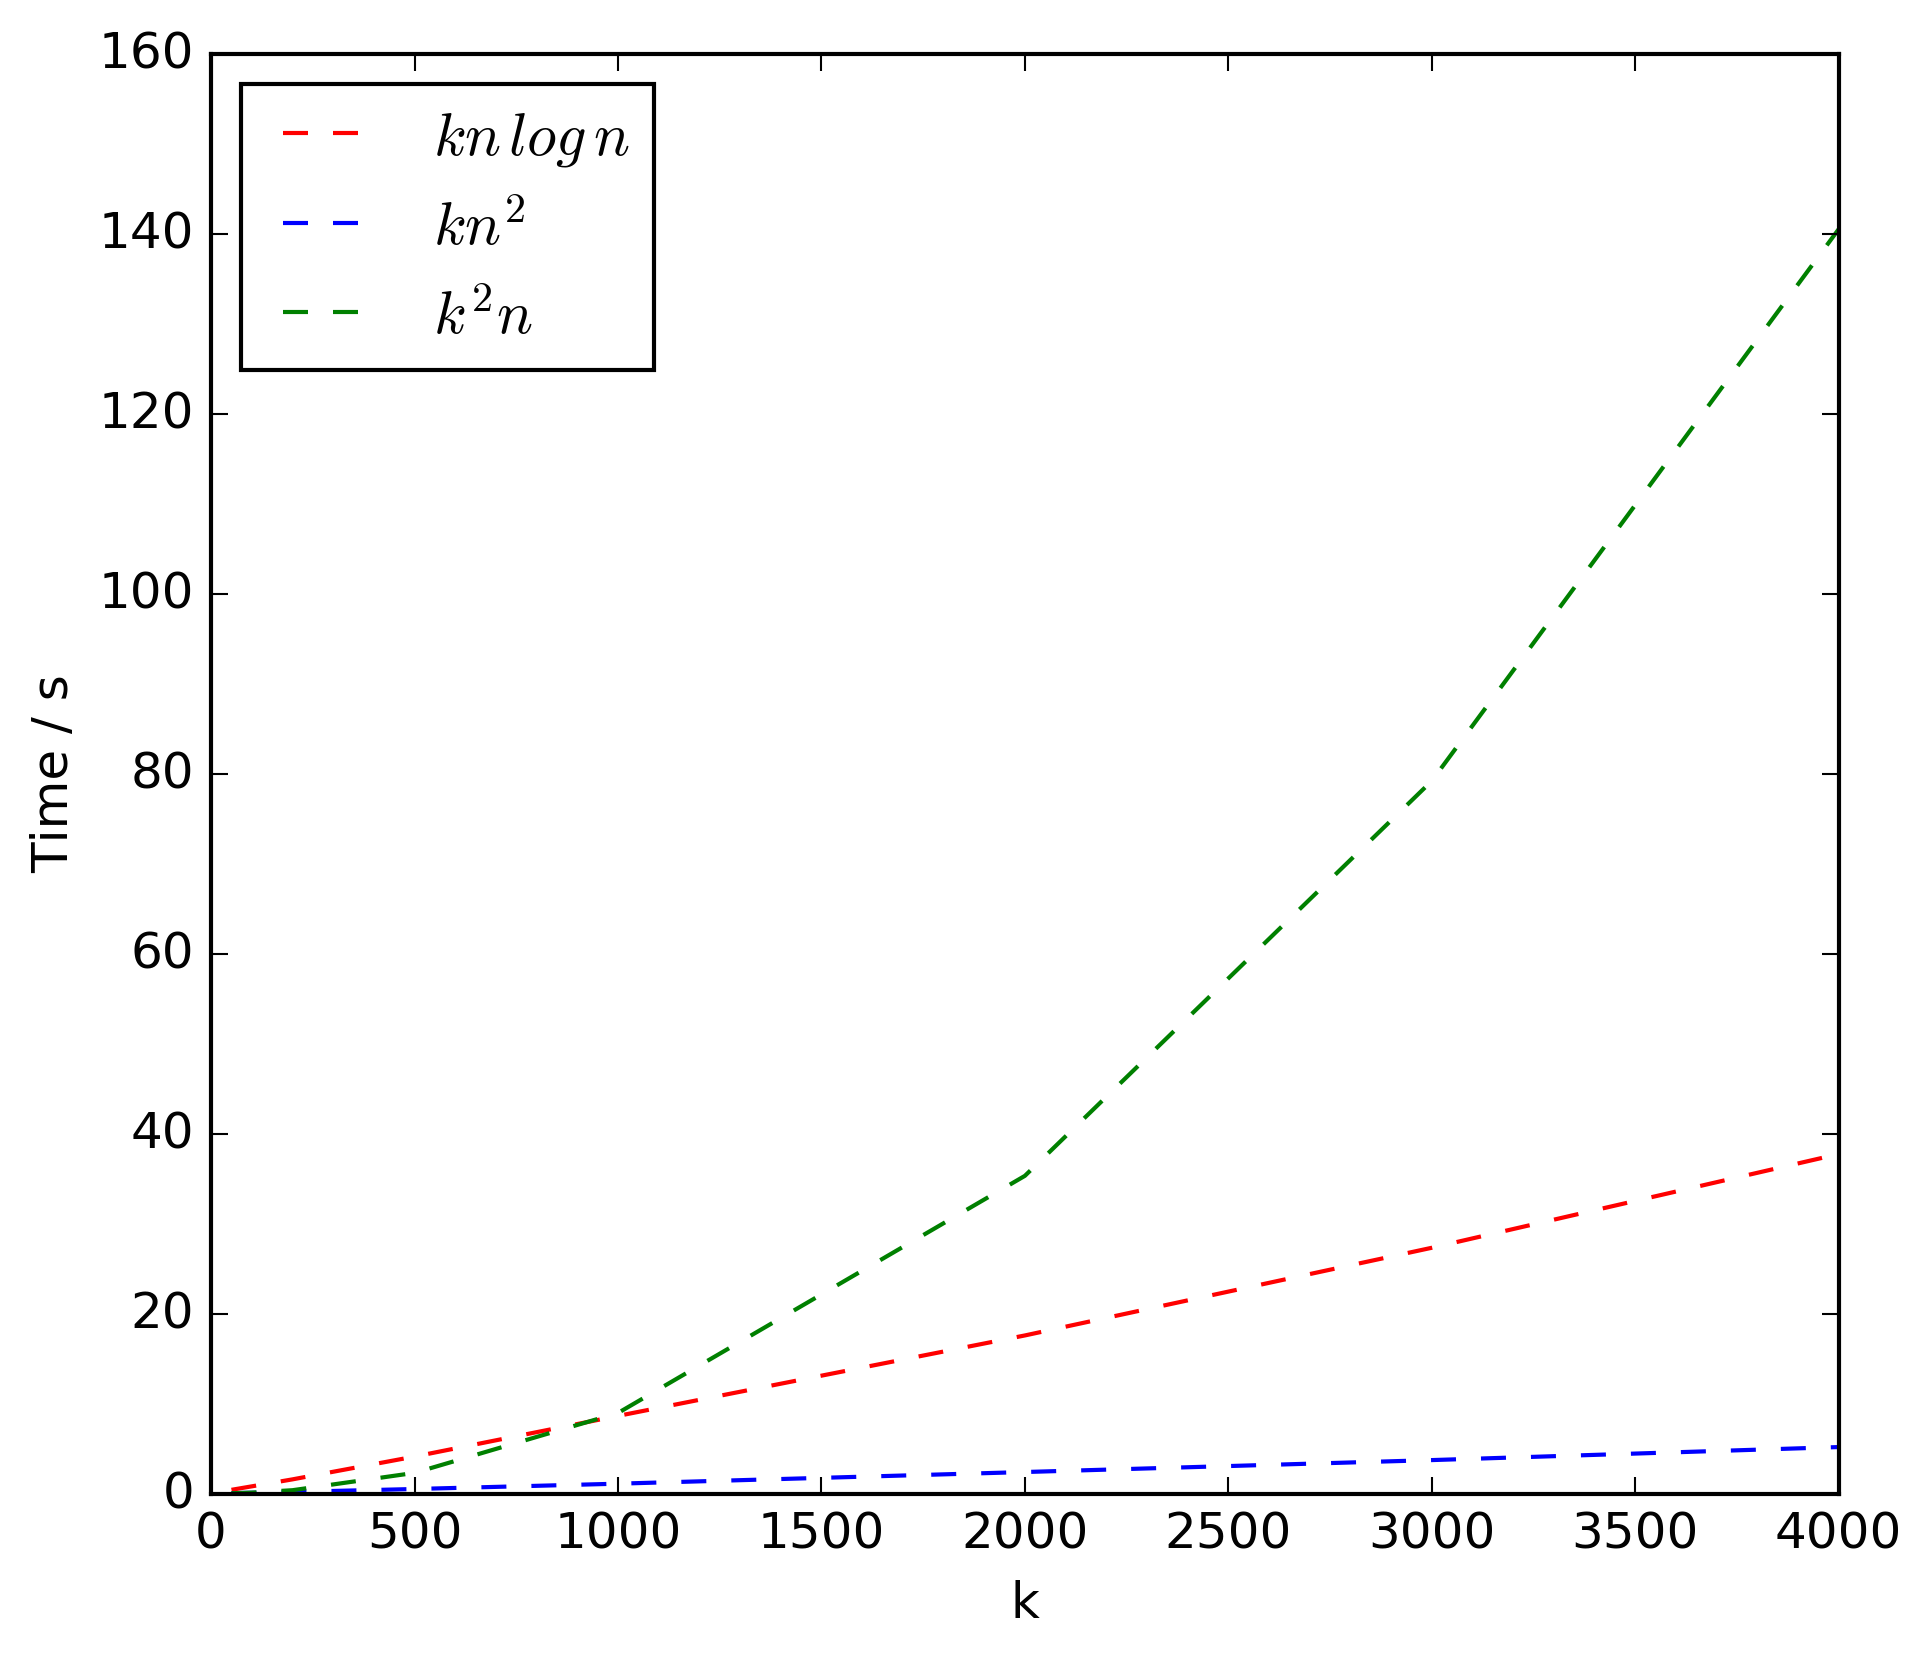
\includegraphics[scale=0.4]{varyingk2_weighting}
            \vspace{0.5cm}
        \end{minipage}\hfill
        \begin{minipage}{0.48\textwidth}
            \centering
            \caption{\texttt{Filter\_Clusters} time with $n = 1000$, varying $k$}
            \label{tab:filterk2}
            \begin{tabular}{c||ccccc}
                $k$ & $n\,log\,n$ & $n\,log^2n$\\
                \hline\hline
                50 & 1.14 & 1.00\\
                100 & 2.18 & 2.78\\
                200 & 4.38 & 5.54\\
                500 & 11.24 & 19.86\\
                1000 & 22.87 & 46.90\\
                2000 & 49.79 & 101.64\\
                3000 & 80.24 & 162.47\\
                4000 & 112.12 & 227.85\\
            \end{tabular}
            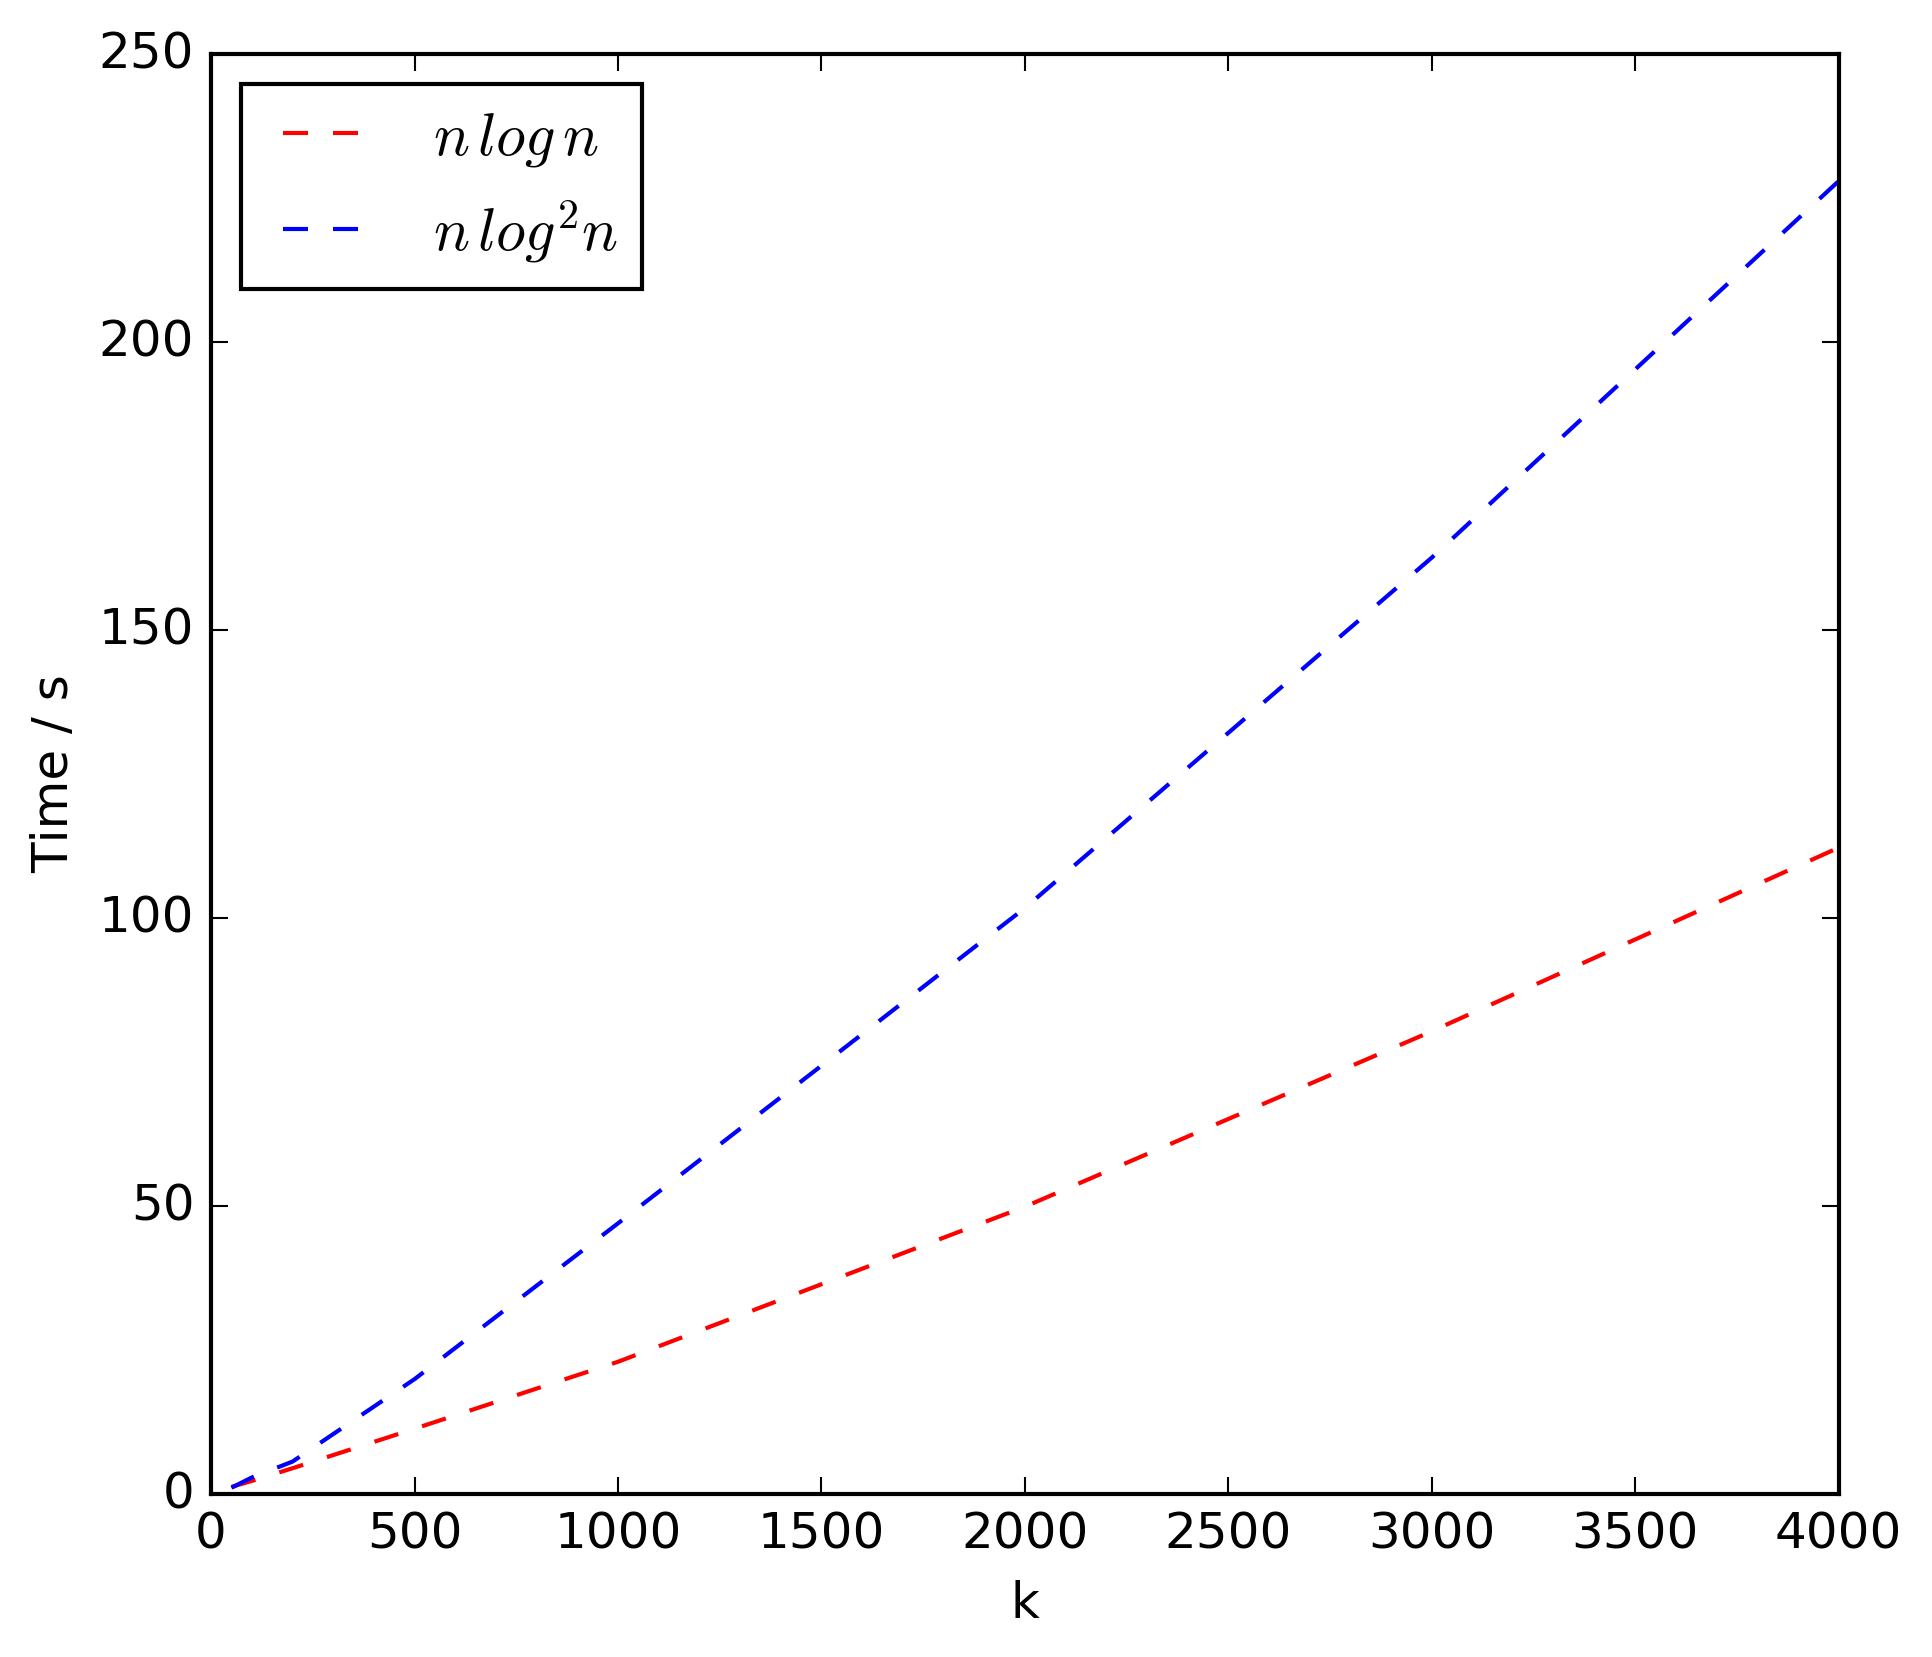
\includegraphics[scale=0.4]{varyingk2_filter}
            \vspace{0.5cm}
        \end{minipage}
        \begin{minipage}{0.48\textwidth}
            \centering
            \caption{Weighting time with $k = 100$, varying $n$}
            \label{tab:weightn2}
            \begin{tabular}{c||ccccc}
                $n$ & $kn\,log\,n$ & $kn^2$ & $k^2n$\\
                \hline\hline
                1000 & 0.75 & 0.08 & 0.09\\
                2000 & 1.68 & 0.25 & 0.20\\
                3000 & 2.68 & 0.43 & 0.29\\
                5000 & 4.77 & 1.05 & 0.48\\
                7500 & 7.56 & 2.07 & 0.76\\
                10000 & 10.59 & 3.62 & 1.01\\
                20000 & 24.49 & 11.11 & 2.08\\
                30000 & 37.76 & 28.42 & 3.18\\
                40000 & 53.57 & 73.68 & 4.42\\
            \end{tabular}
            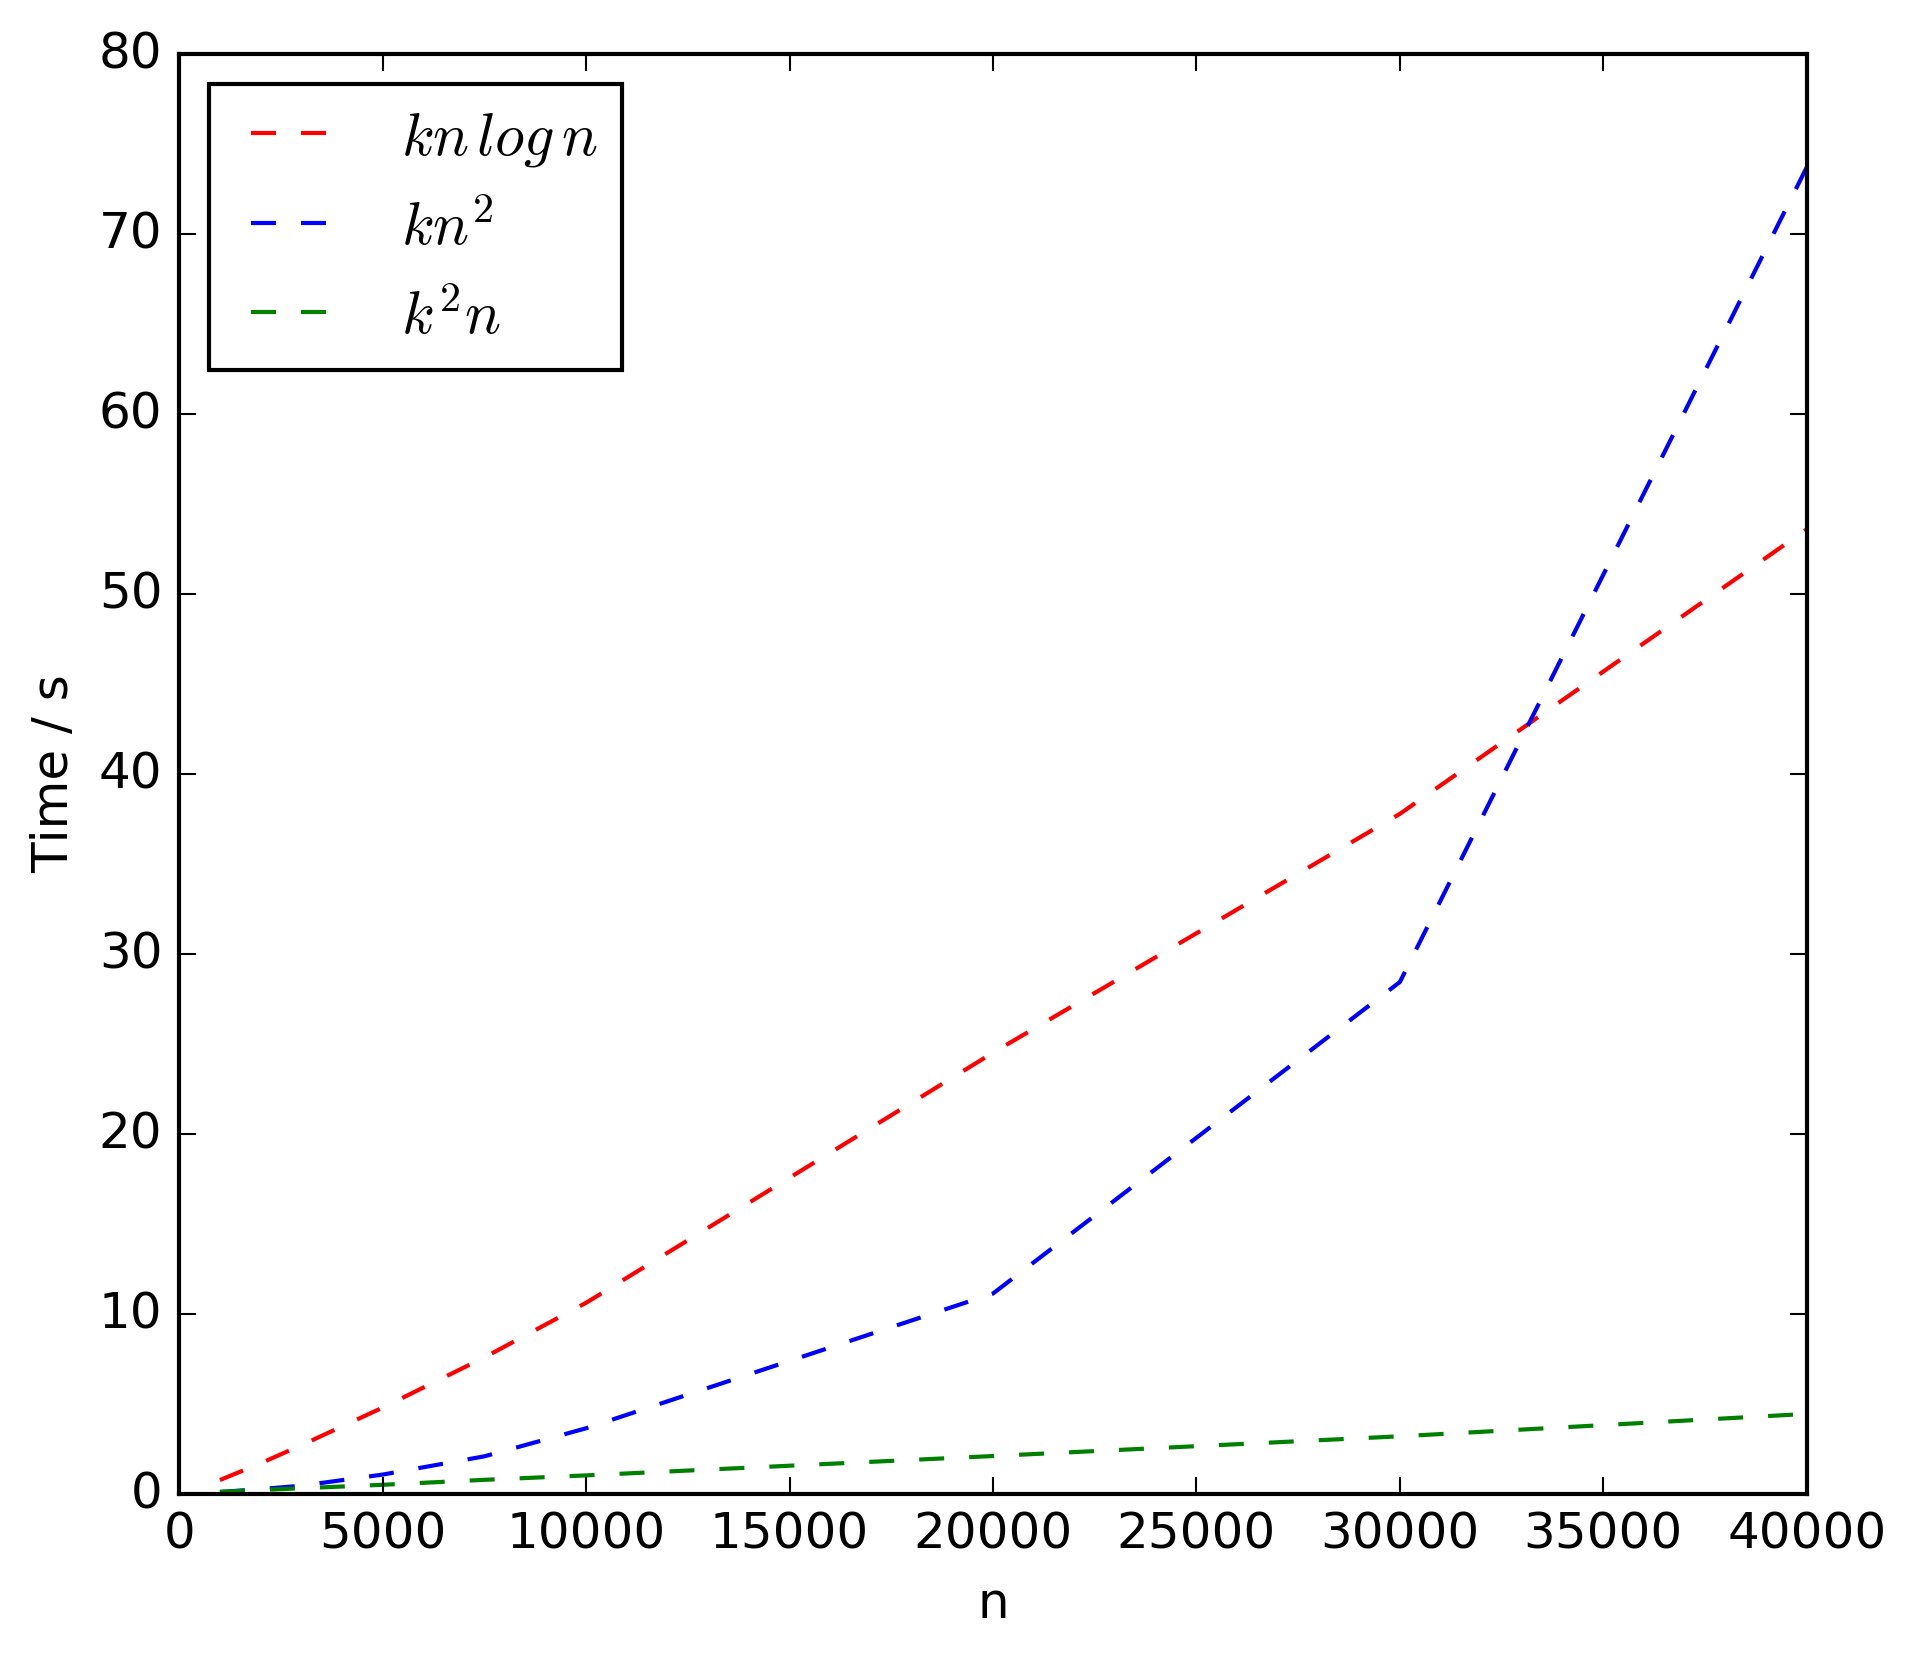
\includegraphics[scale=0.4]{varyingn2_weighting}
        \end{minipage}\hfill
        \begin{minipage}{0.48\textwidth}
            \centering
            \caption{\texttt{Filter\_Clusters} time with $k = 100$, varying $n$}
            \label{tab:filtern2}
            \begin{tabular}{c||ccccc}
                $n$ & $n\,log\,n$ & $n\,log^2n$\\
                \hline\hline
                500 & 1.04 & 0.60\\
                1000 & 2.09 & 2.65\\
                1500 & 3.20 & 7.34\\
                2000 & 4.40 & 11.84\\
                3000 & 6.77 & 20.64\\
                4000 & 9.28 & 32.04\\
                5000 & 11.81 & 45.94\\
                7500 & 18.71 & 90.62\\
                10000 & 26.69 & 150.22\\
            \end{tabular}
            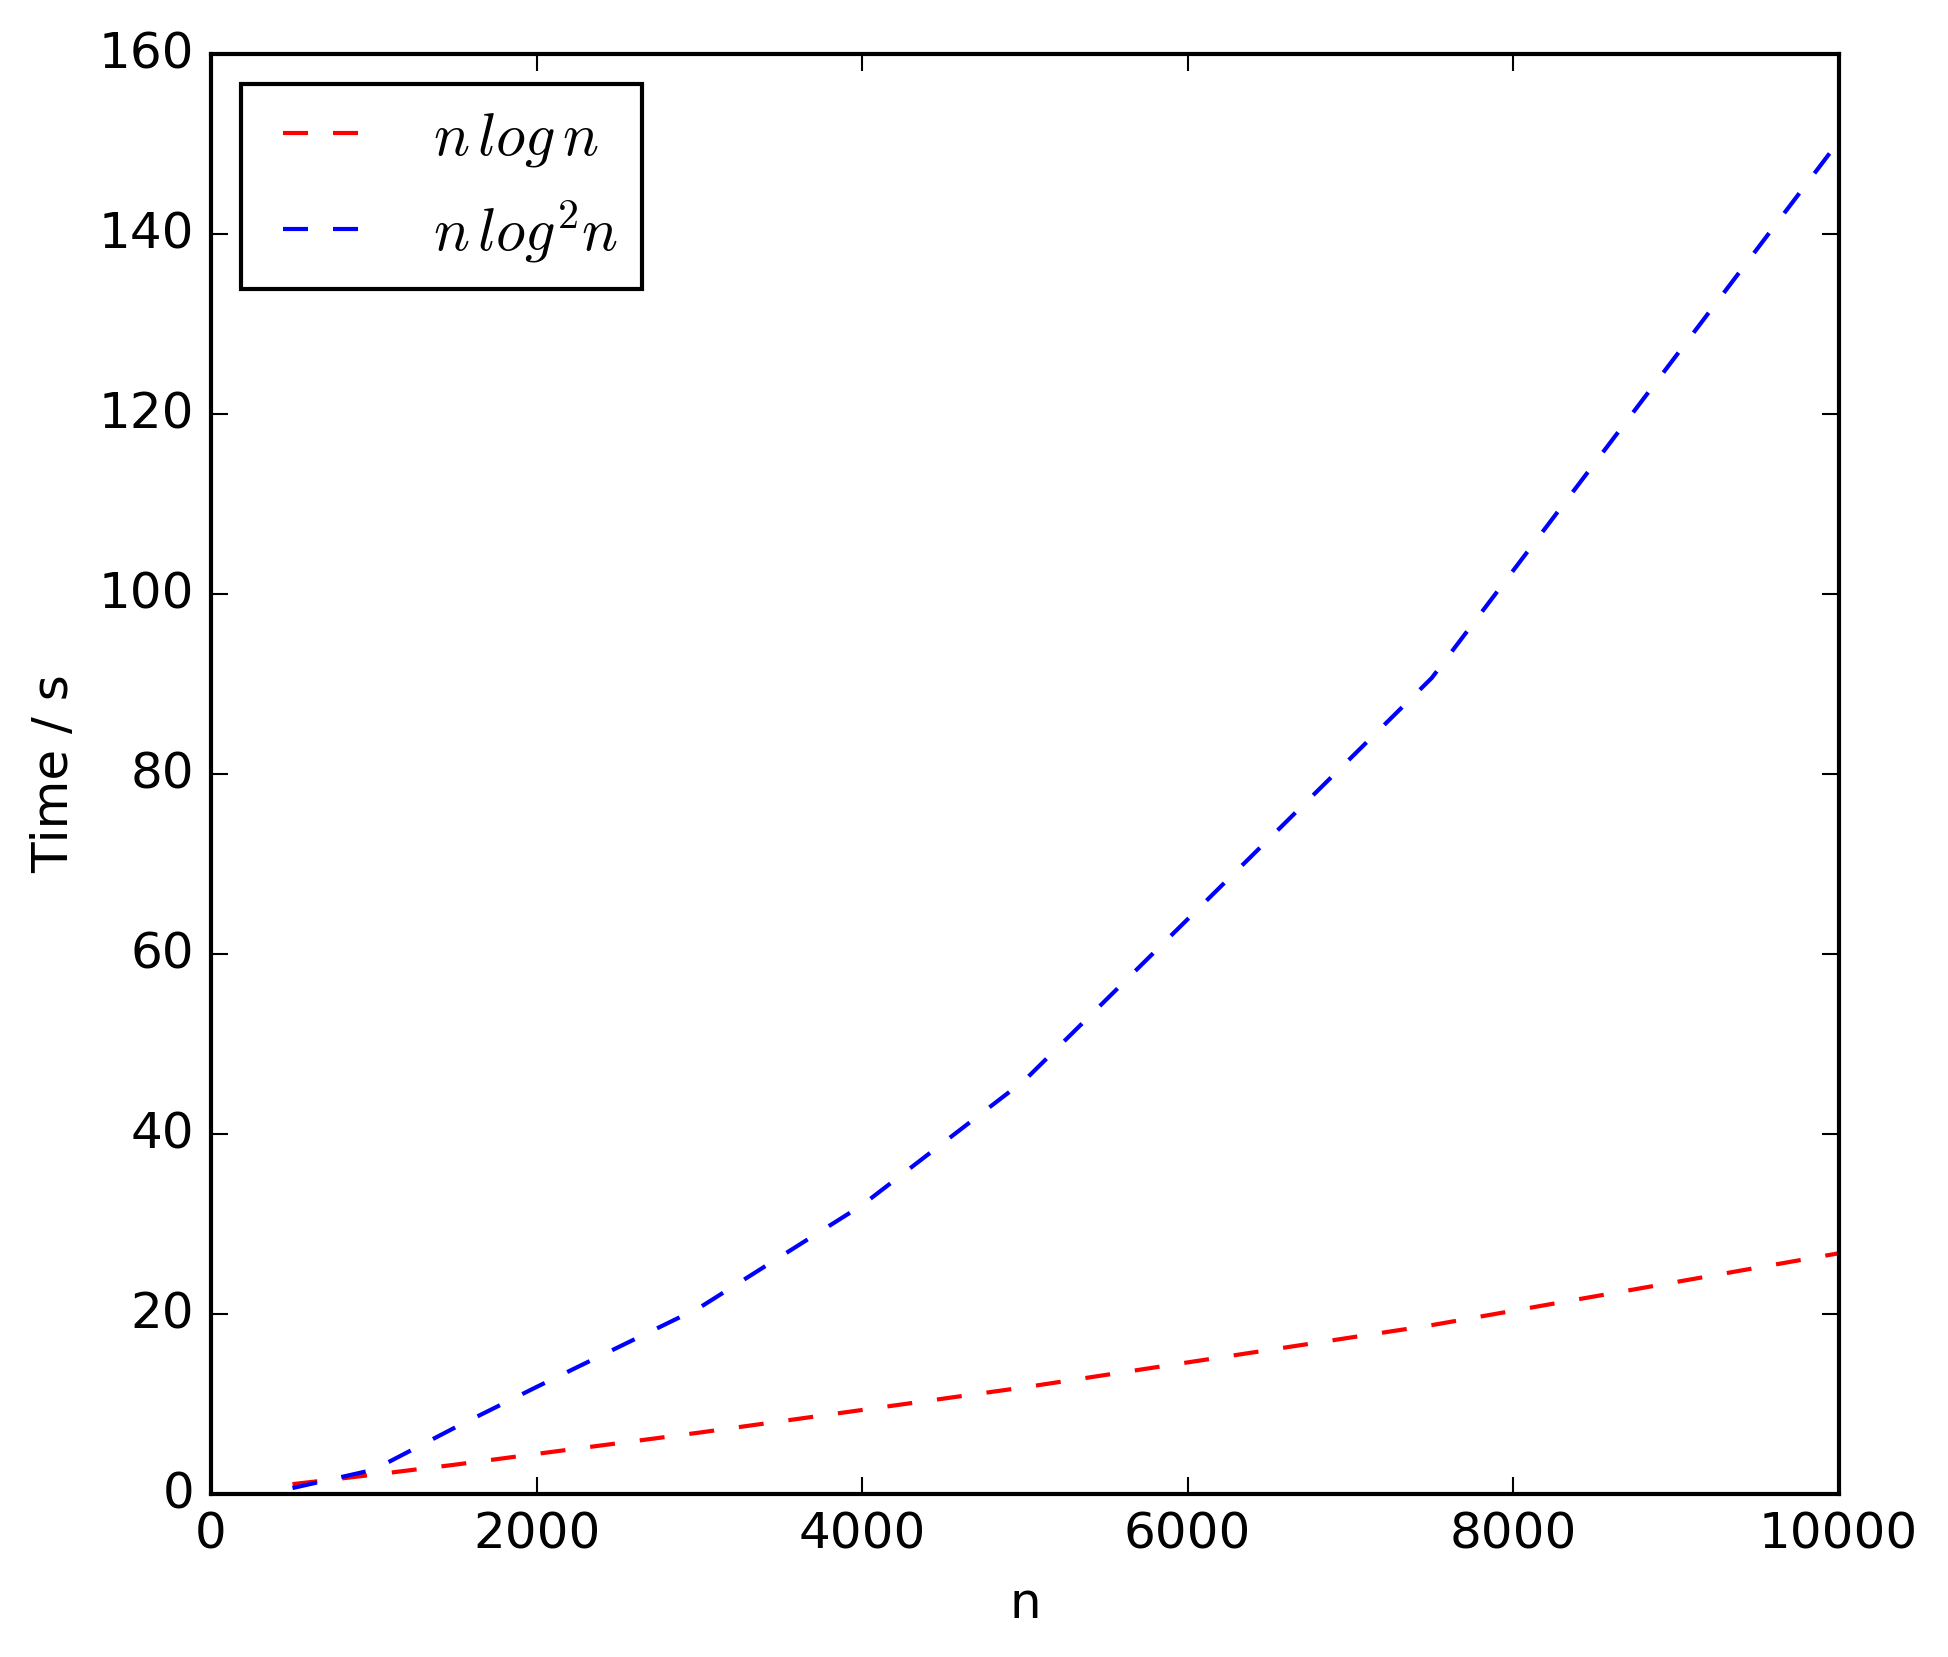
\includegraphics[scale=0.4]{varyingn2_filter}
        \end{minipage}
        \captionof{figure}{Experimental Results for Scenario $2$}
        \label{fig:expresults2}
    \end{table}

    The experimentally observed average running times are given in \cref{tab:weightk1,tab:filterk1,tab:weightn1,tab:filtern1,tab:weightk2,tab:filterk2,tab:weightn2,tab:filtern2}, seen in \cref{fig:expresults1,fig:expresults2}.

    \textit{Comparing Scenarios.} Observe that the basic structure of the graphs across the two scenarios is the same, i.e. we see the same relationships between the various algorithms. An interesting case is to compare Table~\ref{tab:weightn1} and Table~\ref{tab:weightn2}. They show that the $kn\,log\,n$ weighting algorithm performs worse in Scenario 2. This is likely because in Scenario 2 there is a far larger number of distinct clusters, increasing the range of the labels assigned during the weighting step. This leads to the counting/radix sorts becoming less efficient. It can also be seen that the $n\,log^2n$ \texttt{Filter\_Clusters} algorithm performs differently in the two scenarios. Specifically, when we vary $n$, it performs better in Scenario 2 (compare Tables~\ref{tab:filtern1} and~\ref{tab:filtern2}). As pointed out in \cite{jansson2018algorithms}, this is because the larger number of distinct clusters in Scenario 2 leads to more clusters being discarded due to the filtering, due to which the algorithm needs to maintain a smaller tree. We can also see that it performs worse in Scenario 2 when we vary $k$ (compare Tables~\ref{tab:filterk1} and~\ref{tab:filterk2}). To explain this, we note that this implementation in fact uses a simpler version of \texttt{Filter\_Clusters}, with time complexity $O(n^2)$, when $n \leq 1000$. The runtime of this algorithm increases as the number of incompatible nodes increases, and hence it performs worse under Scenario 2. Since our algorithm performs similarly for both scenarios, apart from the discussion above, we will henceforth only be referring to \cref{tab:weightk1,tab:filterk1,tab:weightn1,tab:filtern1}.

    \textit{Weighting Step.} From Table~\ref{tab:weightk1}, it is clear that, as expected, as $k$ increases, the runtime of the $k^2n$ algorithm becomes much worse than that of the other two. Similarly, Table~\ref{tab:weightn1} shows that when $n$ increases, runtime of the $kn^2$ becomes worse than that of the $k^2n$. More interestingly, the algorithm with a theoretical runtime of $kn\,log\,n$ actually performs worse than the $kn^2$ one for values of $n$ up to around $25000$. This is because the constants in the new algorithm are larger, due to the construction of the restricted subtrees. However, we can see that the runtime for the $kn^2$ algorithm is growing faster than the new algorithm, and it does indeed perform worse for very large values of $n$. In practice, though, values of $n$ are not so large, and hence it is likely that the old implementation is better in practice. Also note that, as mentioned in \cite{jansson2018algorithms}, the $kn^2$ algorithm costs memory quadratic in $n$, so if memory is a concern, then using one of the other methods might be more advisable. The choice of which one to use would depend on the value of $k$.

    \texttt{Filter\_Clusters.} Table~\ref{tab:filterk1} is not particularly interesting here since it merely demonstrates that the two algorithms perform similarly when $n = 1000$. However, Table~\ref{tab:filtern1} illustrates that the new algorithm overtakes the old one very quickly when $n > 1000$, performing up to $10$ times better as $n$ nears $10000$. This might be surprising, as the theoretical difference is only a factor of $log\,n$. We (informally) think that this is because of implementation detail 3, due to which we can skip the costly construction of the $\TB||\leafset^{\tau}$ trees. Thus, based on these results, we recommend using the old algorithm if $n \leq 1000$ and the new one otherwise. Note that this would in fact mean using the simpler version of \texttt{Filter\_Clusters}, with time complexity $O(n^2)$, when $n \leq 1000$.

    \section{Conclusion}
    We have given a new deterministic algorithm for constructing the FDCT of a set of phylogenetic trees. This algorithm betters the previously best known one by a factor of $log\,n$. We leave open the problem of finding an optimal solution, i.e. one with time complexity $O(kn)$. Observe that doing so would involve bettering both halves of the algorithm or coming up with a new approach.

%    \newpage
%\bibliographystyle{elsarticle-num}
%\bibliography{final_report}

    \bibliographystyle{plain}
    \bibliography{final_report}
\end{document}
